%%%%%%%%%%%%%%%%%%%%%%%%%%%%%%%%%%%%%%%%%%%%%%%%%%%%%%%%%%%%%%%%%%%%%%%%%%%%%%%%%%%%%%%%%%%%%%%%%%%%%%%%%%%%%%%%%%%%%%%%%%%%%%%%%%%%%%%%%%%%%%%%%%%%%%%%%%%%%%%%%%%%%%%
%%%%%%%%%%%%%%%%%%%%%%%%%%%%%%%%%%%%%%%%%%%%%%%%%%%%%%%%%%%%%%%%%%%%%%%%%%%%%%%%%%%%%%%%%%%%%%%%%%%%%%%%%%%%%%%%%%%%%%%%%%%%%%%%%%%%%%%%%%%%%%%%%%%%%%%%%%%%%%%%%%%%%%%
\chapter{Lifetime reweighting}
\label{app:LifetimeReweighting}
The probability density function of a particle's proper lifetime for a sample generated with a particle's mean lifetime $\tau^{\text{gen}}$ is given by
\begin{equation*}
p \left( t \right) = \frac{1}{\tau^{\text{gen}}} \cdot \exp\left[ -\frac{t}{\tau^{\text{gen}}} \right].
\end{equation*}

After carrying out the lifetime reweighting procedure, the targeted p.d.f of the particle's new mean lifetime $\tau^{\text{target}}$ is given by
\begin{equation*}
p'  \left( t \right) = \frac{1}{\tau^{\text{target}}} \cdot \exp\left[ -\frac{t}{\tau^{\text{target}}} \right].
\end{equation*}
Thus, an event containing a particle with individual proper lifetime can be reweighted with the following weight
\begin{equation*}
\label{eq:reweight}
\frac{p'  \left( t \right)}{p \left( t \right)} = \frac{\tau^{\text{gen}}}{\tau^{\text{target}}} \cdot \exp\left[ \frac{t}{\tau^{\text{gen}}} - \frac{t}{\tau^{\text{target}}} \right].  %= \frac{\tau^{\text{gen}}}{\tau^{\text{target}}} \cdot \exp \left[ t \cdot \left( \frac{1}{\tau^{\text{gen}}} - \frac{1}{\tau^{\text{target}}} \right) \right] .
\end{equation*}
For more than one non-stable particle, the event weight is calculated by multiplying the weights of the single reweighting procedures.

%%%%%%%%%%%%%%%%%%%%%%%%%%%%%%%%%%%%%%%%%%%%%%%%%%%%%%%%%%%%%%%%%%%%%%%%%%%%%%%%%%%%%%%%%%%%%%%%%%%%%%%%%%%%%%%%%%%%%%%%%%%%%%%%%%%%%%%%%%%%%%%%%%%%%%%%%%%%%%%%%%%%%%%
%%%%%%%%%%%%%%%%%%%%%%%%%%%%%%%%%%%%%%%%%%%%%%%%%%%%%%%%%%%%%%%%%%%%%%%%%%%%%%%%%%%%%%%%%%%%%%%%%%%%%%%%%%%%%%%%%%%%%%%%%%%%%%%%%%%%%%%%%%%%%%%%%%%%%%%%%%%%%%%%%%%%%%%
\clearpage
\chapter{Detailed event yield tables for simulated samples and data}
\label{app:cutflow}


\renewcommand{\arraystretch}{1.1}
\begin{table}[!h]
%\begin{sideways}
\centering
\caption{Event yields after each selection step for various background processes. FIXME update this table with correct ttjets sample!!}
\label{tab:CutflowMC}
\makebox[0.99\textwidth]{
\begin{tabular}{|l|c|c|c|c|}
\multicolumn{5}{c}{} \\
\toprule

Selection               &   \WJets  & \ttbarJets  & \Zlep & Multijet  \\
\midrule

after skim ($\pt^{\text{1.jets}}>60\gev$)                                                                             & 9.16 $\cdot10^{7 }$ & 1.04 $\cdot10^{6 }$ & 2.21 $\cdot10^{7 }$ & 1.38 $\cdot10^{11}$ \\
trigger                                                                                   & 4.31 $\cdot10^{6 }$ & 1.12 $\cdot10^{5 }$ & 4.23 $\cdot10^{3 }$ & 4.32 $\cdot10^{6 }$ \\
$\ptfirstjet>100\gev$                                                                     & 3.07 $\cdot10^{6 }$ & 7.89 $\cdot10^{4 }$ & 1.02 $\cdot10^{3 }$ & 1.15 $\cdot10^{6 }$ \\
$\met>100\gev$                                                                            & 1.89 $\cdot10^{6 }$ & 5.17 $\cdot10^{4 }$ & 6.26 $\cdot10^{2 }$ & 9.63 $\cdot10^{5 }$ \\
$\Delta\phi_{\text{max}} \left( \text{jet}_i, \text{jet}_j  \right)<2.7$                     & 1.11 $\cdot10^{6 }$ & 6.58 $\cdot10^{3 }$ & 1.32 $\cdot10^{2 }$ & 9.55 $\cdot10^{3 }$ \\
$\Delta\phi_{\text{max}} \left( \text{jet}_i, \met  \right)>0.5$                             & 1.11 $\cdot10^{6 }$ & 6.64 $\cdot10^{3 }$ & 1.32 $\cdot10^{2 }$ & 2.01 $\cdot10^{4 }$ \\
$\geq1$ reconstructed trk                                                                 & 1.10 $\cdot10^{6 }$ & 6.57 $\cdot10^{3 }$ & 1.32 $\cdot10^{2 }$ & 9.55 $\cdot10^{3 }$ \\
$\geq1$ high-purity trk                                                                   & 1.10 $\cdot10^{6 }$ & 6.57 $\cdot10^{3 }$ & 1.32 $\cdot10^{2 }$ & 9.55 $\cdot10^{3 }$ \\
$\geq1$ trk with $N_{\text{miss}}^{\text{middle}}=0$                                             & 1.09 $\cdot10^{6 }$ & 6.55 $\cdot10^{3 }$ & 1.32 $\cdot10^{2 }$ & 9.55 $\cdot10^{3 }$ \\
$\geq1$ trk with $N_{\text{miss}}^{\text{inner}}=0$                                              & 1.07 $\cdot10^{6 }$ & 6.53 $\cdot10^{3 }$ & 1.32 $\cdot10^{2 }$ & 9.55 $\cdot10^{3 }$ \\
$\geq1$ trk with $|d0|<0.02\cm$                                                           & 1.07 $\cdot10^{6 }$ & 6.47 $\cdot10^{3 }$ & 1.32 $\cdot10^{2 }$ & 9.55 $\cdot10^{3 }$ \\
$\geq1$ trk with $|dz|<0.5\cm$                                                            & 1.07 $\cdot10^{6 }$ & 6.46 $\cdot10^{3 }$ & 1.32 $\cdot10^{2 }$ & 9.55 $\cdot10^{3 }$ \\
$\geq1$ trk with $|\eta|<2.1$                                                             & 1.03 $\cdot10^{6 }$ & 6.41 $\cdot10^{3 }$ & 1.32 $\cdot10^{2 }$ & 9.55 $\cdot10^{3 }$ \\
$\geq1$ trk with $\pt>10\gev$                                                             & 1.03 $\cdot10^{6 }$ & 6.41 $\cdot10^{3 }$ & 1.32 $\cdot10^{2 }$ & 9.55 $\cdot10^{3 }$ \\
$\geq1$ trk without a $\mu$ within $\Delta R<0.15$                                        & 9.85 $\cdot10^{5 }$ & 6.32 $\cdot10^{3 }$ & 1.14 $\cdot10^{2 }$ & 9.55 $\cdot10^{3 }$ \\
$\geq1$ trk without an e within $\Delta R<0.15$                                           & 9.55 $\cdot10^{5 }$ & 6.22 $\cdot10^{3 }$ & 8.53 $\cdot10^{1 }$ & 9.55 $\cdot10^{3 }$ \\
$\geq1$ trk without a $\tau$ within $\Delta R<0.15$                                       & 9.53 $\cdot10^{5 }$ & 6.21 $\cdot10^{3 }$ & 8.53 $\cdot10^{1 }$ & 9.55 $\cdot10^{3 }$ \\
$\geq1$ trk without a jet within $\Delta R<0.5$                                           & 9.15 $\cdot10^{5 }$ & 6.13 $\cdot10^{3 }$ & 8.53 $\cdot10^{1 }$ & 9.55 $\cdot10^{3 }$ \\
\makecell[l]{$\geq1$ trk ! within $\Delta R<0.05$ of \\\hfill a dead/noisy ECAL cell}     & 3.70 $\cdot10^{5 }$ & 3.78 $\cdot10^{3 }$ & 8.53 $\cdot10^{1 }$ & 0.00 $\cdot10^{0 }$ \\
\makecell[l]{$\geq1$ trk ! within an ECAL  intermodule gap}                               & 3.52 $\cdot10^{5 }$ & 3.61 $\cdot10^{3 }$ & 8.53 $\cdot10^{1 }$ & 0.00 $\cdot10^{0 }$ \\
$\geq1$ trk ! within $1.42<|\eta|<1.65$                                                   & 2.21 $\cdot10^{5 }$ & 2.30 $\cdot10^{3 }$ & 0.00 $\cdot10^{0 }$ & 0.00 $\cdot10^{0 }$ \\
$\geq1$ trk ! within $\Delta R<0.25$ to a bad CSC                                         & 1.04 $\cdot10^{4 }$ & 1.20 $\cdot10^{2 }$ & 0.00 $\cdot10^{0 }$ & 0.00 $\cdot10^{0 }$ \\
$\geq1$ trk with $\sum \limits_{\Delta R < 0.3} \pt/p_{\text{T}}^{\text{cand}} < 0.1$     & 8.14 $\cdot10^{3 }$ & 7.96 $\cdot10^{1 }$ & 0.00 $\cdot10^{0 }$ & 0.00 $\cdot10^{0 }$ \\
\bottomrule
\end{tabular}}
%\end{sideways}
\end{table}  
%\end{landscape}

\renewcommand{\arraystretch}{1.1}
\begin{table}[!h]
%\begin{sideways}
\centering
\caption{Event yields after each selection step for various signal models. FIXME update this table with other signal samples!!}
\label{tab:CutflowMC}
\makebox[0.99\textwidth]{
\begin{tabular}{|l|c|c|c|c|}
\multicolumn{5}{c}{} \\
\toprule

\multirow{2}{*}{Selection}                                              &   m=100\gev          &   m=100\gev          &   m=500\gev          &   m=500\gev          \\
                                                                        &   $c\tau$=10\cm      &   $c\tau$=100\cm     &   $c\tau$=10\cm      &   $c\tau$=100\cm      \\
\midrule


before selection                                                                          & 3.41 $\cdot10^{5 }$ & 3.41 $\cdot10^{5 }$ & 3.46 $\cdot10^{2 }$ & 3.46 $\cdot10^{2 }$ \\
trigger                                                                                   & 1.56 $\cdot10^{4 }$ & 1.49 $\cdot10^{4 }$ & 4.63 $\cdot10^{1 }$ & 4.61 $\cdot10^{1 }$ \\
$\ptfirstjet>100\gev$                                                                     & 1.10 $\cdot10^{4 }$ & 1.05 $\cdot10^{4 }$ & 3.65 $\cdot10^{1 }$ & 3.58 $\cdot10^{1 }$ \\
$\met>100\gev$                                                                            & 1.09 $\cdot10^{4 }$ & 9.84 $\cdot10^{3 }$ & 3.63 $\cdot10^{1 }$ & 3.56 $\cdot10^{1 }$ \\
$\Delta\phi_{\text{max}} \left( \text{jet}_i, \text{jet}_j  \right)<2.7$                     & 7.91 $\cdot10^{3 }$ & 6.99 $\cdot10^{3 }$ & 2.76 $\cdot10^{1 }$ & 2.70 $\cdot10^{1 }$ \\
$\Delta\phi_{\text{max}} \left( \text{jet}_i, \met  \right)>0.5$                             & 7.91 $\cdot10^{3 }$ & 7.04 $\cdot10^{3 }$ & 2.77 $\cdot10^{1 }$ & 2.71 $\cdot10^{1 }$ \\
$\geq1$ reconstructed trk                                                                 & 3.13 $\cdot10^{3 }$ & 5.75 $\cdot10^{3 }$ & 5.74 $\cdot10^{0 }$ & 2.13 $\cdot10^{1 }$ \\
$\geq1$ high-purity trk                                                                   & 2.91 $\cdot10^{3 }$ & 5.66 $\cdot10^{3 }$ & 5.25 $\cdot10^{0 }$ & 2.08 $\cdot10^{1 }$ \\
$\geq1$ trk with $N_{\text{miss}}^{\text{middle}}=0$                                      & 2.87 $\cdot10^{3 }$ & 5.46 $\cdot10^{3 }$ & 5.23 $\cdot10^{0 }$ & 2.02 $\cdot10^{1 }$ \\
$\geq1$ trk with $N_{\text{miss}}^{\text{inner}}=0$                                       & 2.86 $\cdot10^{3 }$ & 5.41 $\cdot10^{3 }$ & 5.22 $\cdot10^{0 }$ & 2.01 $\cdot10^{1 }$ \\
$\geq1$ trk with $|d0|<0.02\cm$                                                           & 2.81 $\cdot10^{3 }$ & 5.39 $\cdot10^{3 }$ & 5.08 $\cdot10^{0 }$ & 1.99 $\cdot10^{1 }$ \\
$\geq1$ trk with $|dz|<0.5\cm$                                                            & 2.80 $\cdot10^{3 }$ & 5.39 $\cdot10^{3 }$ & 5.08 $\cdot10^{0 }$ & 1.99 $\cdot10^{1 }$ \\
$\geq1$ trk with $|\eta|<2.1$                                                             & 2.63 $\cdot10^{3 }$ & 4.98 $\cdot10^{3 }$ & 5.01 $\cdot10^{0 }$ & 1.91 $\cdot10^{1 }$ \\
$\geq1$ trk with $\pt>10\gev$                                                             & 2.63 $\cdot10^{3 }$ & 4.98 $\cdot10^{3 }$ & 5.01 $\cdot10^{0 }$ & 1.91 $\cdot10^{1 }$ \\
$\geq1$ trk without a $\mu$ within $\Delta R<0.15$                                        & 2.63 $\cdot10^{3 }$ & 4.70 $\cdot10^{3 }$ & 5.01 $\cdot10^{0 }$ & 1.89 $\cdot10^{1 }$ \\
$\geq1$ trk without an e within $\Delta R<0.15$                                           & 2.63 $\cdot10^{3 }$ & 4.70 $\cdot10^{3 }$ & 5.01 $\cdot10^{0 }$ & 1.89 $\cdot10^{1 }$ \\
$\geq1$ trk without a $\tau$ within $\Delta R<0.15$                                       & 2.63 $\cdot10^{3 }$ & 4.68 $\cdot10^{3 }$ & 5.01 $\cdot10^{0 }$ & 1.89 $\cdot10^{1 }$ \\
$\geq1$ trk without a jet within $\Delta R<0.5$                                           & 2.61 $\cdot10^{3 }$ & 4.64 $\cdot10^{3 }$ & 4.89 $\cdot10^{0 }$ & 1.84 $\cdot10^{1 }$ \\
\makecell[l]{$\geq1$ trk !within $\Delta R<0.05$ of \\\hfill a dead/noisy ECAL cell}     & 2.40 $\cdot10^{3 }$ & 4.30 $\cdot10^{3 }$ & 4.44 $\cdot10^{0 }$ & 1.71 $\cdot10^{1 }$ \\
\makecell[l]{$\geq1$ trk !within an ECAL  intermodule gap}                               & 2.38 $\cdot10^{3 }$ & 4.27 $\cdot10^{3 }$ & 4.41 $\cdot10^{0 }$ & 1.70 $\cdot10^{1 }$ \\
$\geq1$ trk !within $1.42<|\eta|<1.65$                                                   & 2.16 $\cdot10^{3 }$ & 3.92 $\cdot10^{3 }$ & 4.19 $\cdot10^{0 }$ & 1.58 $\cdot10^{1 }$ \\
$\geq1$ trk !within $\Delta R<0.25$ to a bad CSC                                         & 2.06 $\cdot10^{3 }$ & 3.71 $\cdot10^{3 }$ & 4.06 $\cdot10^{0 }$ & 1.52 $\cdot10^{1 }$ \\
$\geq1$ trk with $\sum \limits_{\Delta R < 0.3} \pt/p_{\text{T}}^{\text{cand}} < 0.1$     & 2.03 $\cdot10^{3 }$ & 3.67 $\cdot10^{3 }$ & 4.00 $\cdot10^{0 }$ & 1.51 $\cdot10^{1 }$ \\
\bottomrule
\end{tabular}}
%\end{sideways}
\end{table}  
%\end{landscape}


%%%%%%%%%%%%%%%%%%%%%%%%%%%%%%%%%%%%%%%%%%%%%%%%%%%%%%%%%%%%%%%%%%%%%%%%%%%%%%%%%%%%%%%%%%%%%%%%%%%%%%%%%%%%%%%%%%%%%%%%%%%%%%%%%%%%%%%%%%%%%%%%%%%%%%%%%%%%%%%%%%%%%%%%%%%%%%%%%%%%
%%%%%%%%%%%%%%%%%%%%%%%%%%%%%%%%%%%%%%%%%%%%%%%%%%%%%%%%%%%%%%%%%%%%%%%%%%%%%%%%%%%%%%%%%%%%%%%%%%%%%%%%%%%%%%%%%%%%%%%%%%%%%%%%%%%%%%%%%%%%%%%%%%%%%%%%%%%%%%%%%%%%%%%%%%%%%%%%%%%%
\clearpage
\chapter{Validation tests of the background estimation methods}
\label{app:Validation}


\renewcommand{\arraystretch}{1.2}
\begin{table}[!h]
\centering
\caption{Validation tests of the background estimation methods in the calorimeter isolation control region $\ecalo>10\gev$ 
         for two different \pt selection requirements:
         $\pt>40\gev$ (left) and $\pt>60\gev$ (right). Only statistical uncertainties are included.}
\label{tab:LeptonicClosure}
\makebox[0.99\textwidth]{
\begin{tabular}{l|c |c}
\multicolumn{3}{c}{} \\
\toprule
                                                               &      Predicted Yield                   &   Data Yield          \\
\midrule
Total bkg        &$84.36^{+16.47}_{-10.88}$                   &94 \\
\midrule
 Electrons        &$15.69^{+11.92}_{-6.72}$                   & \\
     Muons        &$5.67^{+7.74}_{-3.55}$                     & \\
      Taus        &$35.78^{+5.09}_{-4.18}$                    & \\
     Fakes        &$27.23^{+6.57}_{-6.57}$                    & \\
\bottomrule
\multicolumn{3}{c}{} \\
\end{tabular}
\hspace{10pt}
\begin{tabular}{l|c |c}
\multicolumn{3}{c}{} \\
\toprule
                                                               &      Predicted Yield                   &   Data Yield          \\
\midrule
 Total bkg        &$35.56^{+11.95}_{-6.20}$                   &53 \\
\midrule
Electrons        &$0.00^{+9.14}_{-0.00}$                & \\
     Muons        &$3.65^{+4.98}_{-2.28}$                & \\
      Taus        &$13.22^{+1.88}_{-1.55}$                & \\
     Fakes        &$18.70^{+5.55}_{-5.55}$                & \\
\bottomrule
\multicolumn{3}{c}{} \\
\end{tabular}}
\end{table}

\renewcommand{\arraystretch}{1.2}
\begin{table}[!h]
\centering
\caption{Validation tests of the background estimation methods in the calorimeter isolation control region $\ecalo>10\gev$
         with an additional \ias selection of $\ias>0.2$ for two different \pt selection requirements:
         $\pt>40\gev$ (left) and $\pt>60\gev$ (right). Only statistical uncertainties are included.}
\label{tab:LeptonicClosure}
\makebox[0.99\textwidth]{
\begin{tabular}{l|c |c}
\multicolumn{3}{c}{} \\
\toprule
                                                               &      Predicted Yield                   &   Data Yield          \\
\midrule
 Total bkg        &$4.76^{+1.42}_{-1.39}$                   &8 \\
\midrule
Electrons        &$0.20^{+0.17}_{-0.10}$                & \\
     Muons        &$0.00^{+0.22}_{-0.00}$                & \\
      Taus        &$0.48^{+0.15}_{-0.11}$                & \\
     Fakes        &$4.08^{+1.38}_{-1.38}$                & \\
\bottomrule
\multicolumn{3}{c}{} \\
\end{tabular}
\hspace{10pt}
\begin{tabular}{l|c |c}
\multicolumn{3}{c}{} \\
\toprule
                                                               &      Predicted Yield                   &   Data Yield          \\
\midrule
 Total bkg        &$2.31^{+0.97}_{-0.95}$                   &3 \\
\midrule
 Electrons        &$0.00^{+0.11}_{-0.00}$                & \\
     Muons        &$0.00^{+0.14}_{-0.00}$                & \\
      Taus        &$0.18^{+0.06}_{-0.04}$                & \\
     Fakes        &$2.14^{+0.95}_{-0.95}$                & \\
 \bottomrule
\multicolumn{3}{c}{} \\
\end{tabular}}
\end{table}

\renewcommand{\arraystretch}{1.2}
\begin{table}[!h]
\centering
\caption{Validation tests of the background estimation methods in the calorimeter isolation control region $\ecalo>10\gev$
         with an additional \ias selection of $\ias>0.4$ for two different \pt selection requirements:
         $\pt>40\gev$ (left) and $\pt>60\gev$ (right). Only statistical uncertainties are included.}
\label{tab:LeptonicClosure}
\makebox[0.99\textwidth]{
\begin{tabular}{l|c |c}
\multicolumn{3}{c}{} \\
\toprule
                                                               &      Predicted Yield                   &   Data Yield          \\
\midrule
 Total bkg        &$1.98^{+0.87}_{-0.83}$                   &2 \\
\midrule
Electrons        &$0.00^{+0.05}_{-0.00}$                & \\
     Muons        &$0.00^{+0.22}_{-0.00}$                & \\
      Taus        &$0.08^{+0.09}_{-0.04}$                & \\
     Fakes        &$1.91^{+0.83}_{-0.83}$                & \\
\bottomrule
\multicolumn{3}{c}{} \\
\end{tabular}
\hspace{10pt}
\begin{tabular}{l|c |c}
\multicolumn{3}{c}{} \\
\toprule
                                                               &      Predicted Yield                   &   Data Yield          \\
\midrule

 Total bkg        &$1.10^{+0.63}_{-0.61}$                   &1 \\
\midrule
 Electrons        &$0.00^{+0.00}_{-0.00}$                & \\
     Muons        &$0.00^{+0.14}_{-0.00}$                & \\
      Taus        &$0.03^{+0.03}_{-0.02}$                & \\
     Fakes        &$1.07^{+0.61}_{-0.61}$                & \\
\bottomrule
\multicolumn{3}{c}{} \\
\end{tabular}}
\end{table}


\newpage 
The underprediction in the control regions with $\ias>0.2$ is caused by the pediction of the leptonic \ias shape from simulation.
This leads to a bias as the \ias distribution in simulation is softer than in data.
However, this bias is taken into account as systematic uncertainty (see Section~\ref{sec:LeptonIasUncertainty}).


%%%%%%%%%%%%%%%%%%%%%%%%%%%%%%%%%%%%%%%%%%%%%%%%%%%%%%%%%%%%%%%%%%%%%%%%%%%%%%%%%%%%%%%%%%%%%%%%%%%%%%%%%%%%%%%%%%%%%%%%%%%%%%%%%%%%%%%%%%%%%%%%%%%%%%%%%%%%%%%%%%%%%%%%%%%%%%%%%%%%
%%%%%%%%%%%%%%%%%%%%%%%%%%%%%%%%%%%%%%%%%%%%%%%%%%%%%%%%%%%%%%%%%%%%%%%%%%%%%%%%%%%%%%%%%%%%%%%%%%%%%%%%%%%%%%%%%%%%%%%%%%%%%%%%%%%%%%%%%%%%%%%%%%%%%%%%%%%%%%%%%%%%%%%%%%%%%%%%%%%%
\clearpage
\chapter{Selection requirements of the ``tag-and-probe'' samples}
\label{app:TagAndProbeRequirements}

\renewcommand{\arraystretch}{1.4}
\begin{table}[!h]
\centering
\caption{Event selection cuts for the muon ``tag-and-probe'' samples (T\&P signal region sample and T\&P lepton veto inverted control region sample) that are used to estimate the uncertainty on the muon scale factor \muonscalefactor.}
\label{tab:MuonTagAndProbeSample}
\makebox[0.99\textwidth]{
\begin{tabular}{l|l }
\multicolumn{2}{c}{} \\
\toprule
\multirow{10}{*}{\makecell[l]{Muon selection}}                 & $\pt>25\gev$ \\
                                                               & $|\eta|<2.4$ \\
                                                               & $\sum\limits_{\Delta R<0.4} \pt^{\text{PF particle}}/\pt(\mu)<0.12$ \\
                                                               & $\left.\frac{\chi^2}{ndof}\right\rvert_{\text{global track}}<10$ \\
                                                               & $|d0|<0.2\cm$  \\
                                                               & $|dz|<0.5\cm$  \\
                                                               & $\geq$ 1 hit in the muon detector  \\
                                                               & $\geq$ 2 hits in different muon detector planes  \\
                                                               & $\geq$ 1 hit in the pixel detector  \\
                                                               & $\geq$ 6 hits in the tracker system  \\
\midrule
\multirow{6}{*}{Candidate track selection}                     &  Good quality selection \\
                                                               &  Kinematic selection    \\
                                                               &  \makecell[l]{Lepton/jet veto ($\mu$ veto inverted for the\\\hspace{2.7cm} ``tag-and-probe'' control region)}       \\   
                                                               &  Isolation selection    \\  
                                                               &  $\nhits>5$             \\  
\midrule
\multirow{2}{*}{Event-based selection}                         &  Muon and candidate track opposite in charge                                     \\
                                                               &  $80\gev<M_{\text{inv}}\left(\mu,\text{can. trk} \right)<100\gev$        \\

\bottomrule
\multicolumn{2}{c}{} \\
\end{tabular}}
\end{table}

\renewcommand{\arraystretch}{1.4}
\begin{table}[!h]
\centering
\caption{Event selection cuts for the tau ``tag-and-probe'' samples (T\&P signal region sample and T\&P lepton veto inverted control region sample) that are used to estimate the uncertainty on the tau scale factor \tauscalefactor.}
\label{tab:TauTagAndProbeSample}
\makebox[0.99\textwidth]{
\begin{tabular}{l|l }
\multicolumn{2}{c}{} \\
\toprule
\multirow{10}{*}{\makecell[l]{Muon selection\\ that is compatible with a \\$\tau\rightarrow\mu\nu\nu$ decay}}                 & $\pt>25\gev$ \\
                                                               & $|\eta|<2.4$ \\
                                                               & $\sum\limits_{\Delta R<0.4} \pt^{\text{PF particle}}/\pt(\mu)<0.12$ \\
                                                               & $\left.\frac{\chi^2}{ndof}\right\rvert_{\text{global track}}<10$ \\
                                                               & $|d0|<0.2\cm$  \\
                                                               & $|dz|<0.5\cm$  \\
                                                               & $\geq$ 1 hit in the muon detector  \\
                                                               & $\geq$ 2 hits in different muon detector planes  \\
                                                               & $\geq$ 1 hit in the pixel detector  \\
                                                               & $\geq$ 6 hits in the tracker system  \\
\midrule
\multirow{6}{*}{Candidate track selection}                     &  Good quality selection \\
                                                               &  Kinematic selection    \\
                                                               &  \makecell[l]{Lepton/jet veto ($\tau$ veto inverted for the\\\hspace{2.7cm} ``tag-and-probe'' control region)}       \\   
                                                               &  $\sum \limits_{\Delta R < 0.3} \pt/p_{\text{T}}^{\text{cand}} < 0.1$\\  
                                                               &  $\nhits>5$             \\  
\midrule
\multirow{2}{*}{Event-based selection}                         &  Muon and candidate track opposite in charge                                     \\
                                                               &  $40\gev<M_{\text{inv}}\left( \mu, \text{cand. trk}  \right)<75\gev$        \\
                                                               & $m_T\left(\mu,\met\right)<40\gev$ \\

\bottomrule
\multicolumn{2}{c}{} \\
\end{tabular}}
\end{table}


\renewcommand{\arraystretch}{1.4}
\begin{table}[!h]
\centering
\caption{Event selection cuts for the electron ``tag-and-probe'' samples (T\&P signal region sample and T\&P lepton veto inverted control region sample) that are used to estimate the uncertainty on the electron scale factor \electronscalefactor.}
\label{tab:ElectronTagAndProbeSample}
\makebox[0.99\textwidth]{
\begin{tabular}{l|l}
\multicolumn{2}{c}{} \\
\toprule
\multirow{6}{*}{Electron selection}                            &  $\pt>25\gev$ \\
                                                               &  $|\eta|<2.5$ \\
                                                               &  $\sum\limits_{\Delta R<0.4} \pt^{\text{PF particle}}/\pt(e)<0.15$ \\
                                                               &  pass conversion veto    \\
                                                               &  no missing tracker hits  \\
                                                               &  good MVA electron as defined in \cite{bib:CMS:ElectronMVA}  \\
\midrule
\multirow{6}{*}{Candidate track selection}                    &  Good quality selection \\
                                                              &  Kinematic selection    \\
                                                              &   \makecell[l]{Lepton/jet veto ($e$ veto inverted for the\\\hspace{2.7cm} ``tag-and-probe'' control region)}       \\   
                                                              &  $\sum \limits_{\Delta R < 0.3} \pt/p_{\text{T}}^{\text{cand}} < 0.1$    \\  
                                                              &  $\nhits>5$             \\  
\midrule
\multirow{2}{*}{Event-based selection}                         &  Electron and candidate track opposite in charge                      \\
                                                               &  $80\gev<M_{\text{inv}}\left(e,\text{cand. trk}  \right)<100\gev$        \\

\bottomrule
\multicolumn{2}{c}{} \\
\end{tabular}}
\end{table}  

%%%%%%%%%%%%%%%%%%%%%%%%%%%%%%%%%%%%%%%%%%%%%%%%%%%%%%%%%%%%%%%%%%%%%%%%%%%%%%%%%%%%%%%%%%%%%%%%%%%%%%%%%%%%%%%%%%%%%%%%%%%%%%%%%%%%%%%%%%%%%%%%%%%%%%%%%%%%%%%%%%%%%%%
%%%%%%%%%%%%%%%%%%%%%%%%%%%%%%%%%%%%%%%%%%%%%%%%%%%%%%%%%%%%%%%%%%%%%%%%%%%%%%%%%%%%%%%%%%%%%%%%%%%%%%%%%%%%%%%%%%%%%%%%%%%%%%%%%%%%%%%%%%%%%%%%%%%%%%%%%%%%%%%%%%%%%%%
\clearpage
\chapter{Underlying distributions for the qualitative search sensitivity optimisation}
\label{app:OptimisationApp}

\begin{figure}[!h]
  \centering 
  \begin{tabular}{c}
    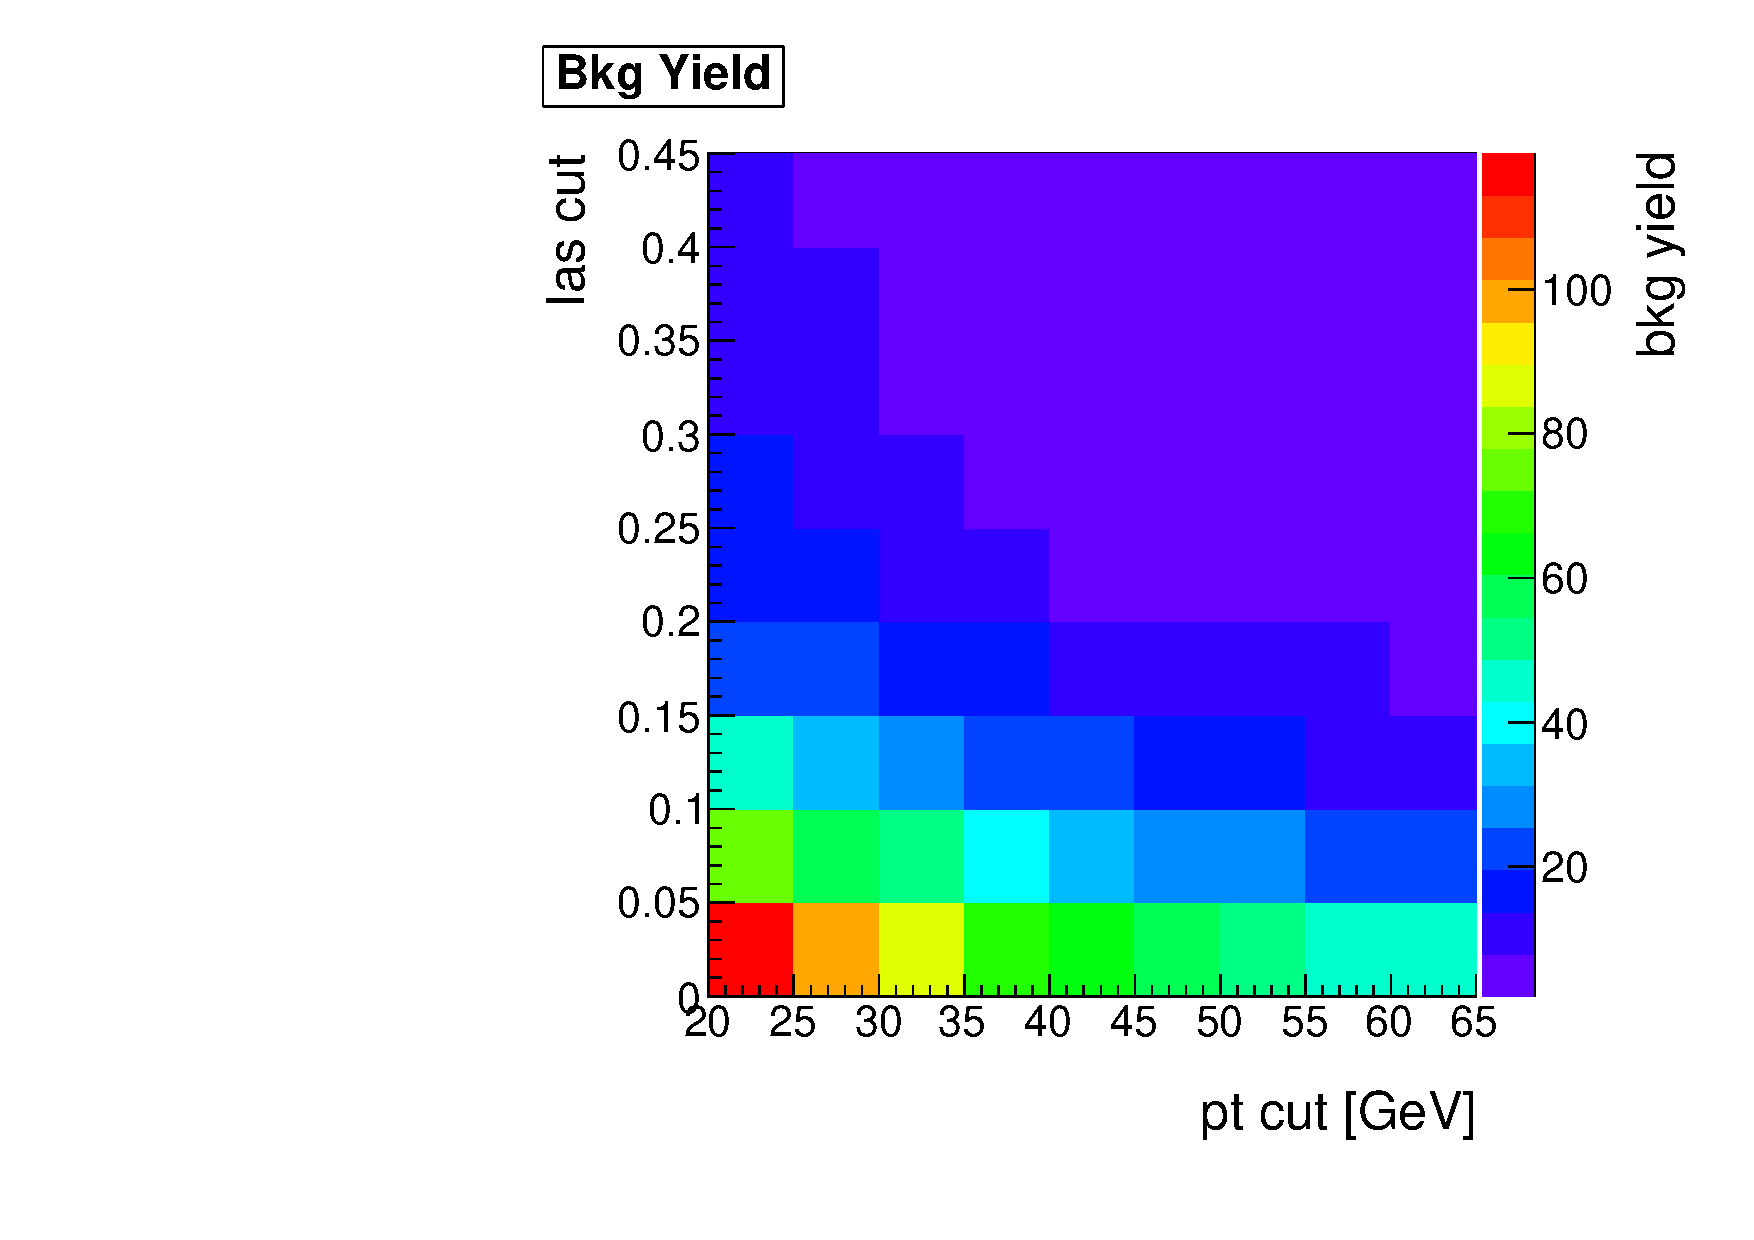
\includegraphics[width=0.35\textwidth]{figures/analysis/Optimisation/BkgYield_ECaloLe5.pdf} 
    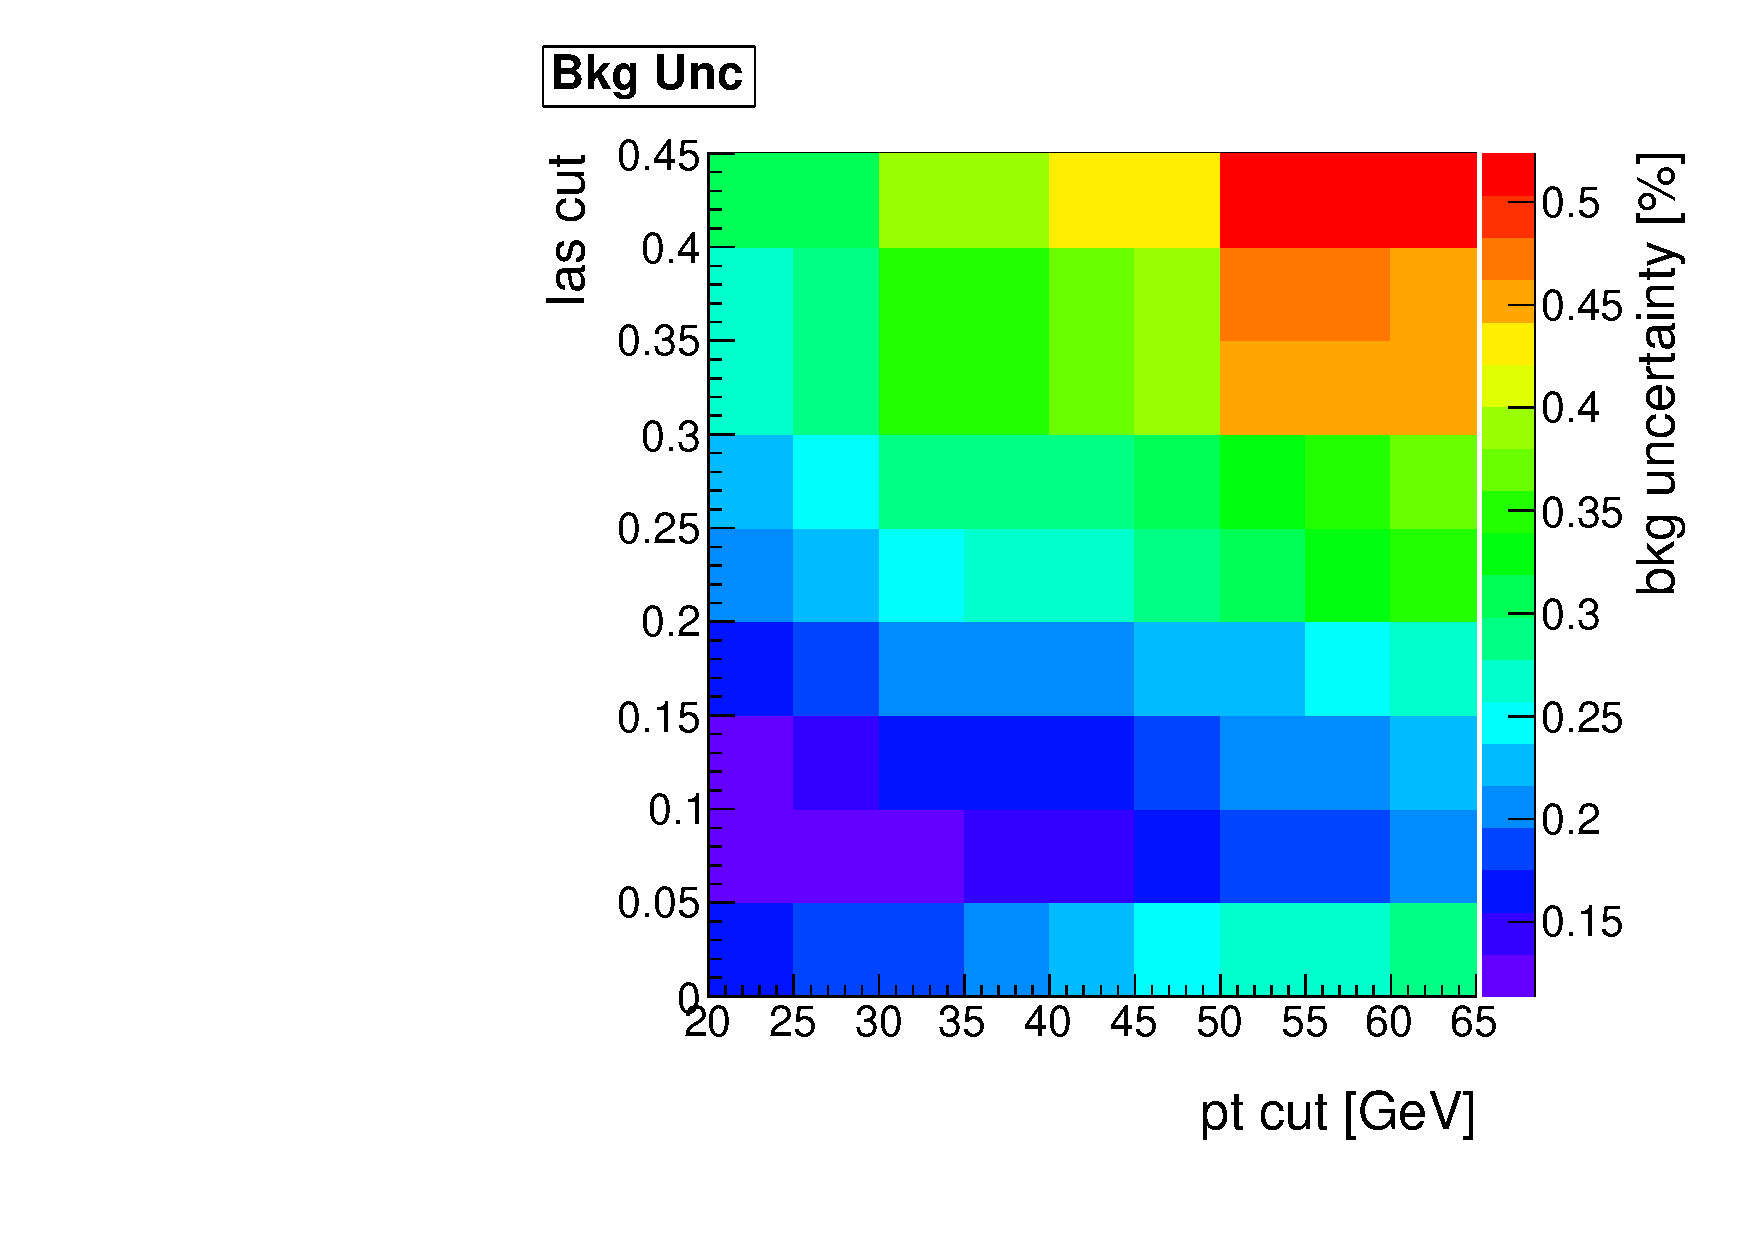
\includegraphics[width=0.35\textwidth]{figures/analysis/Optimisation/BkgUncertainty_ECaloLe5.pdf}\\ 
    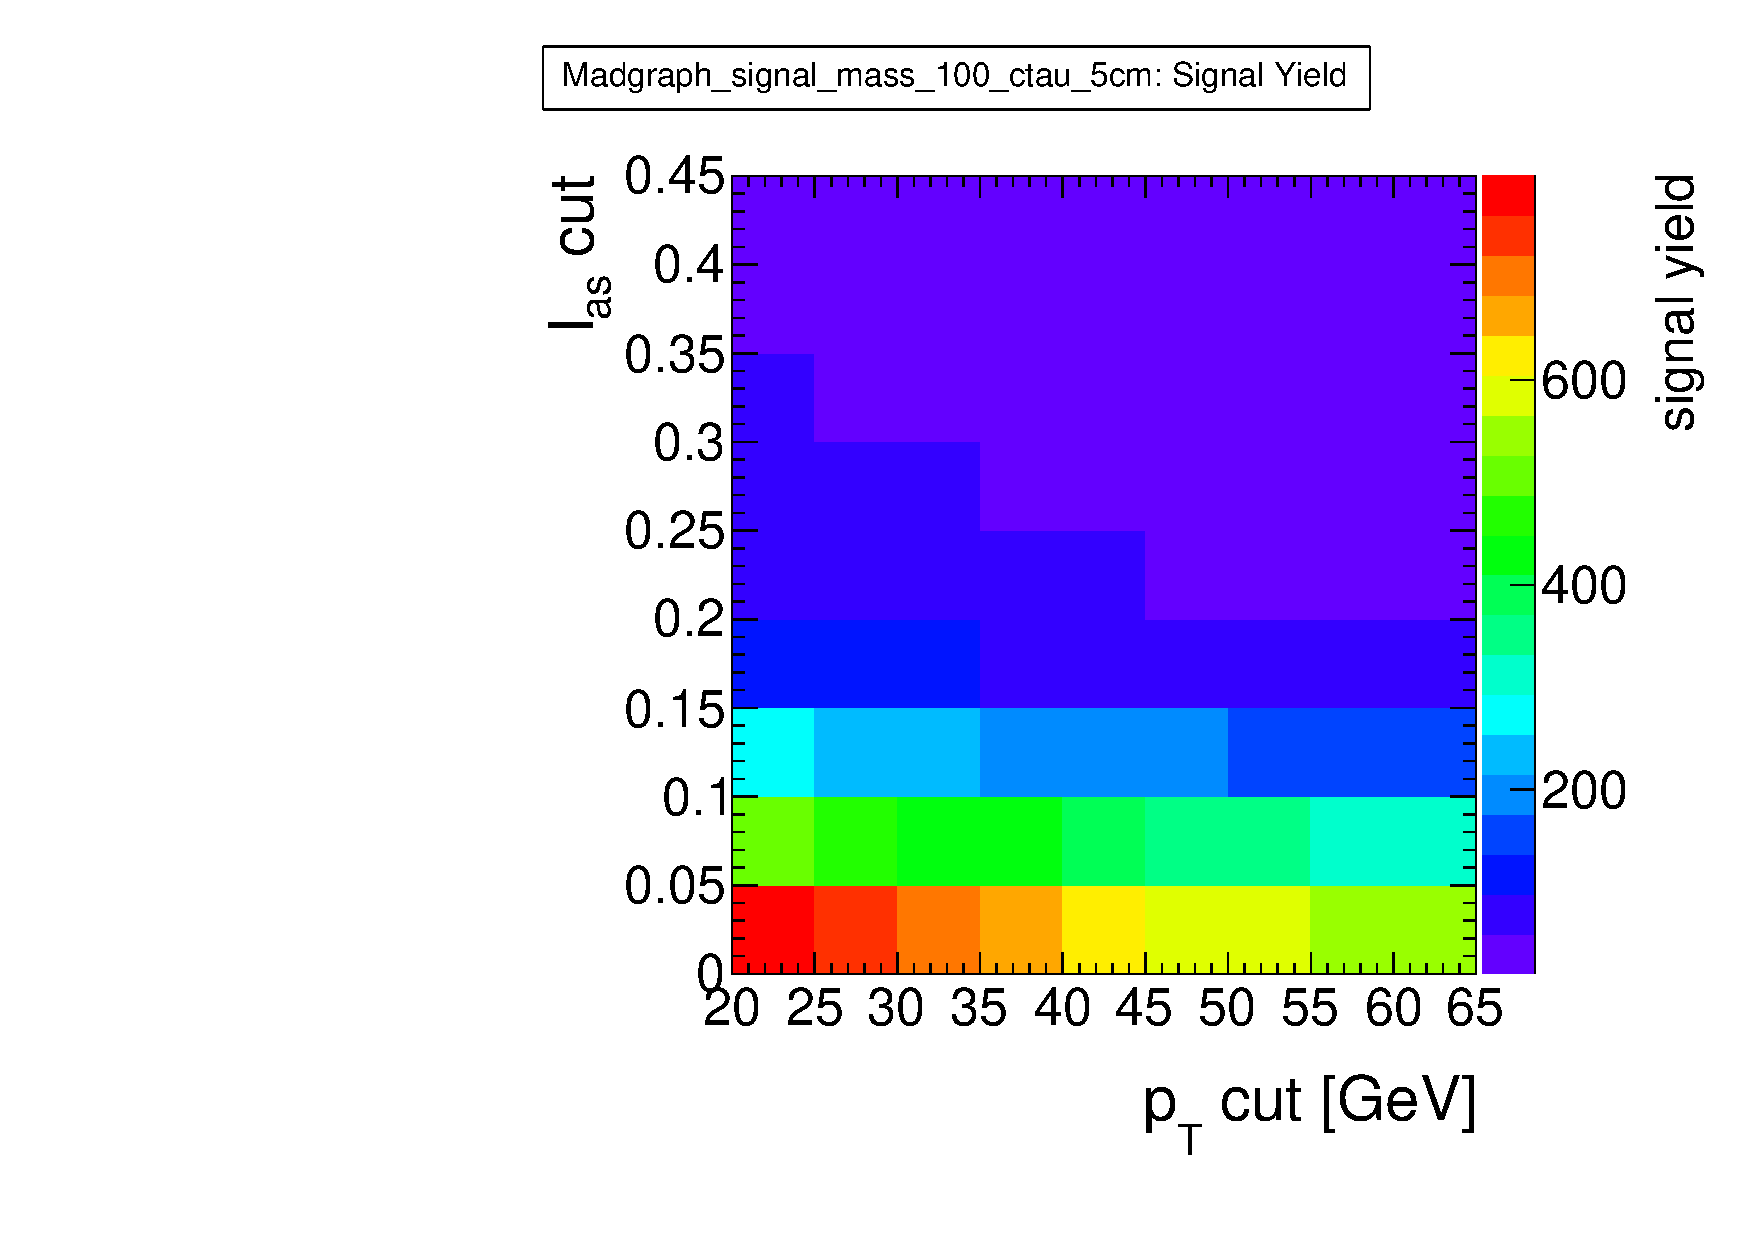
\includegraphics[width=0.35\textwidth]{figures/analysis/Optimisation/Madgraph_signal_mass_100_ctau_5cm_ECaloLe5_SignalYield.pdf}
    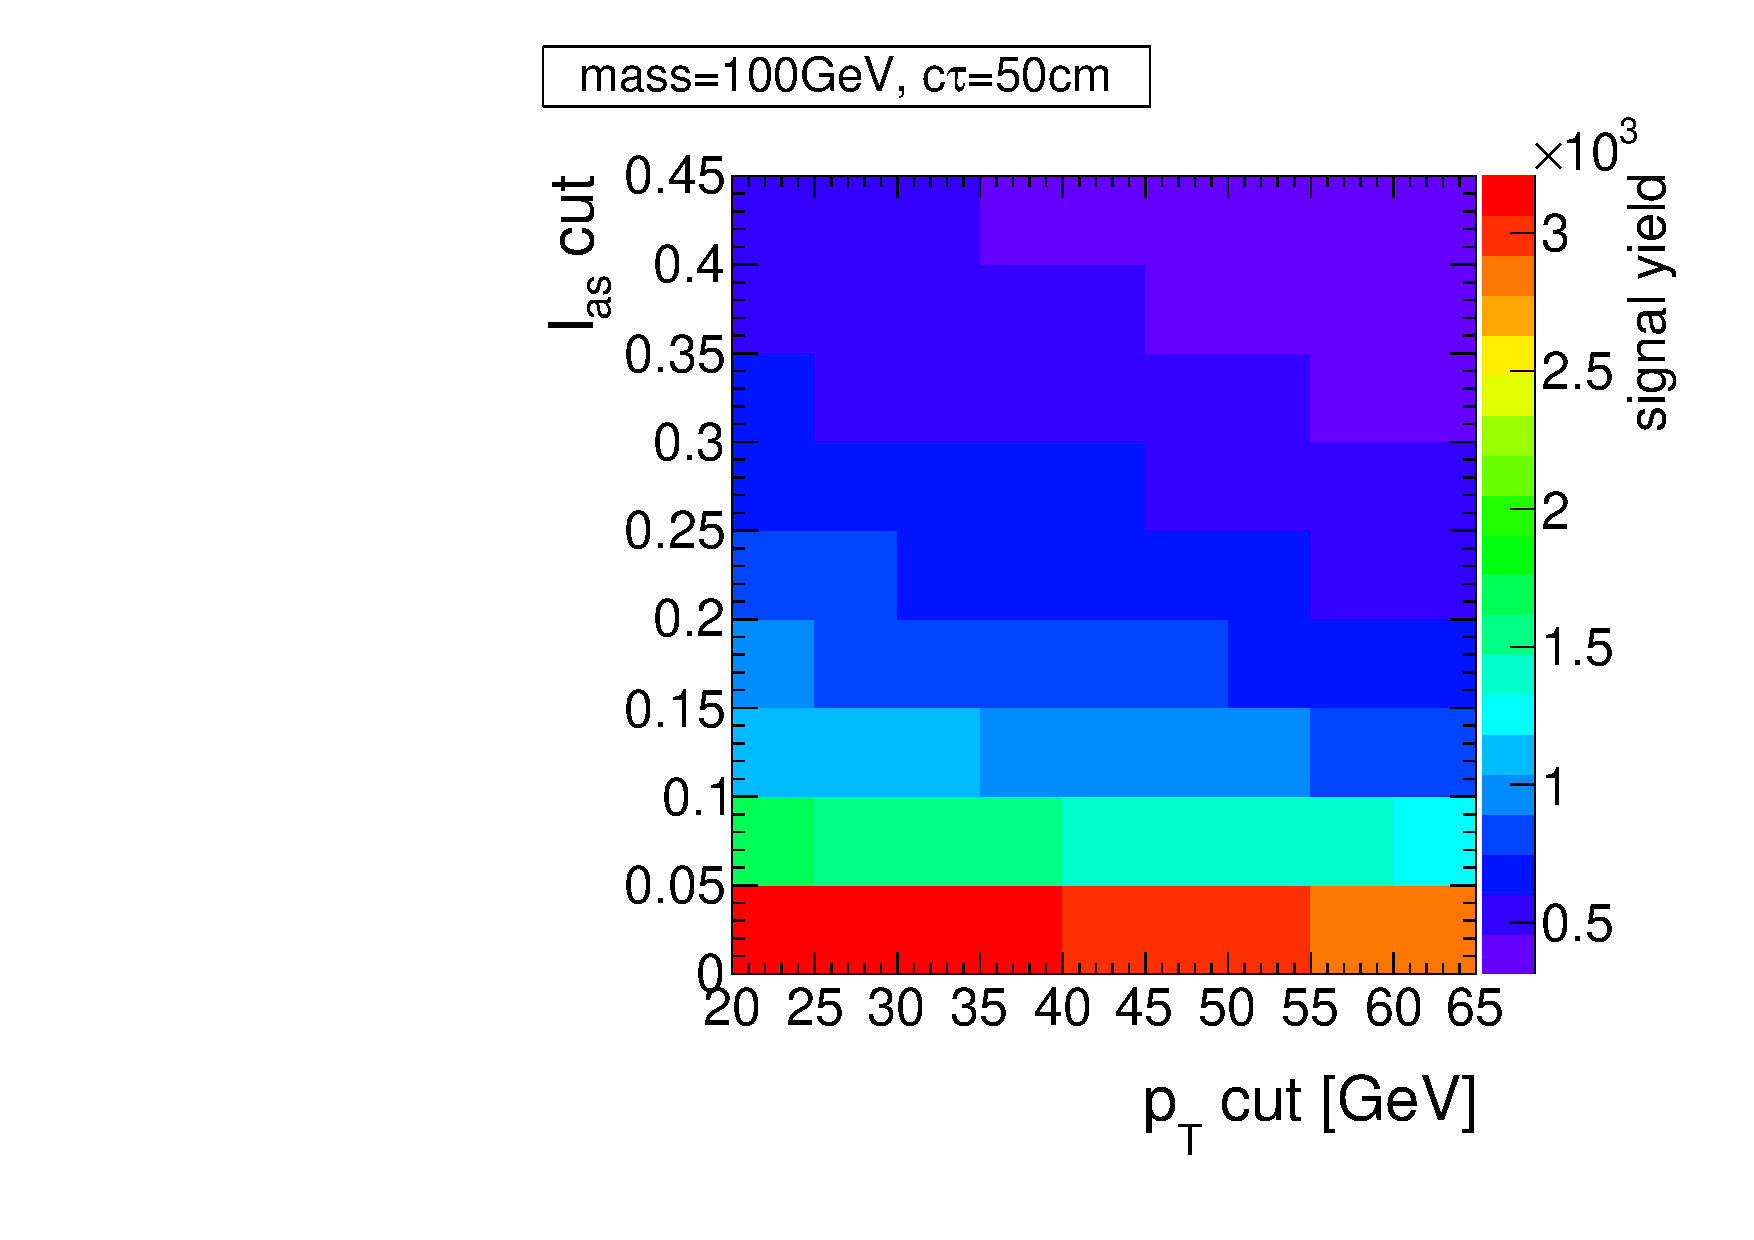
\includegraphics[width=0.35\textwidth]{figures/analysis/Optimisation/Madgraph_signal_mass_100_ctau_50cm_ECaloLe5_SignalYield.pdf}\\ 
    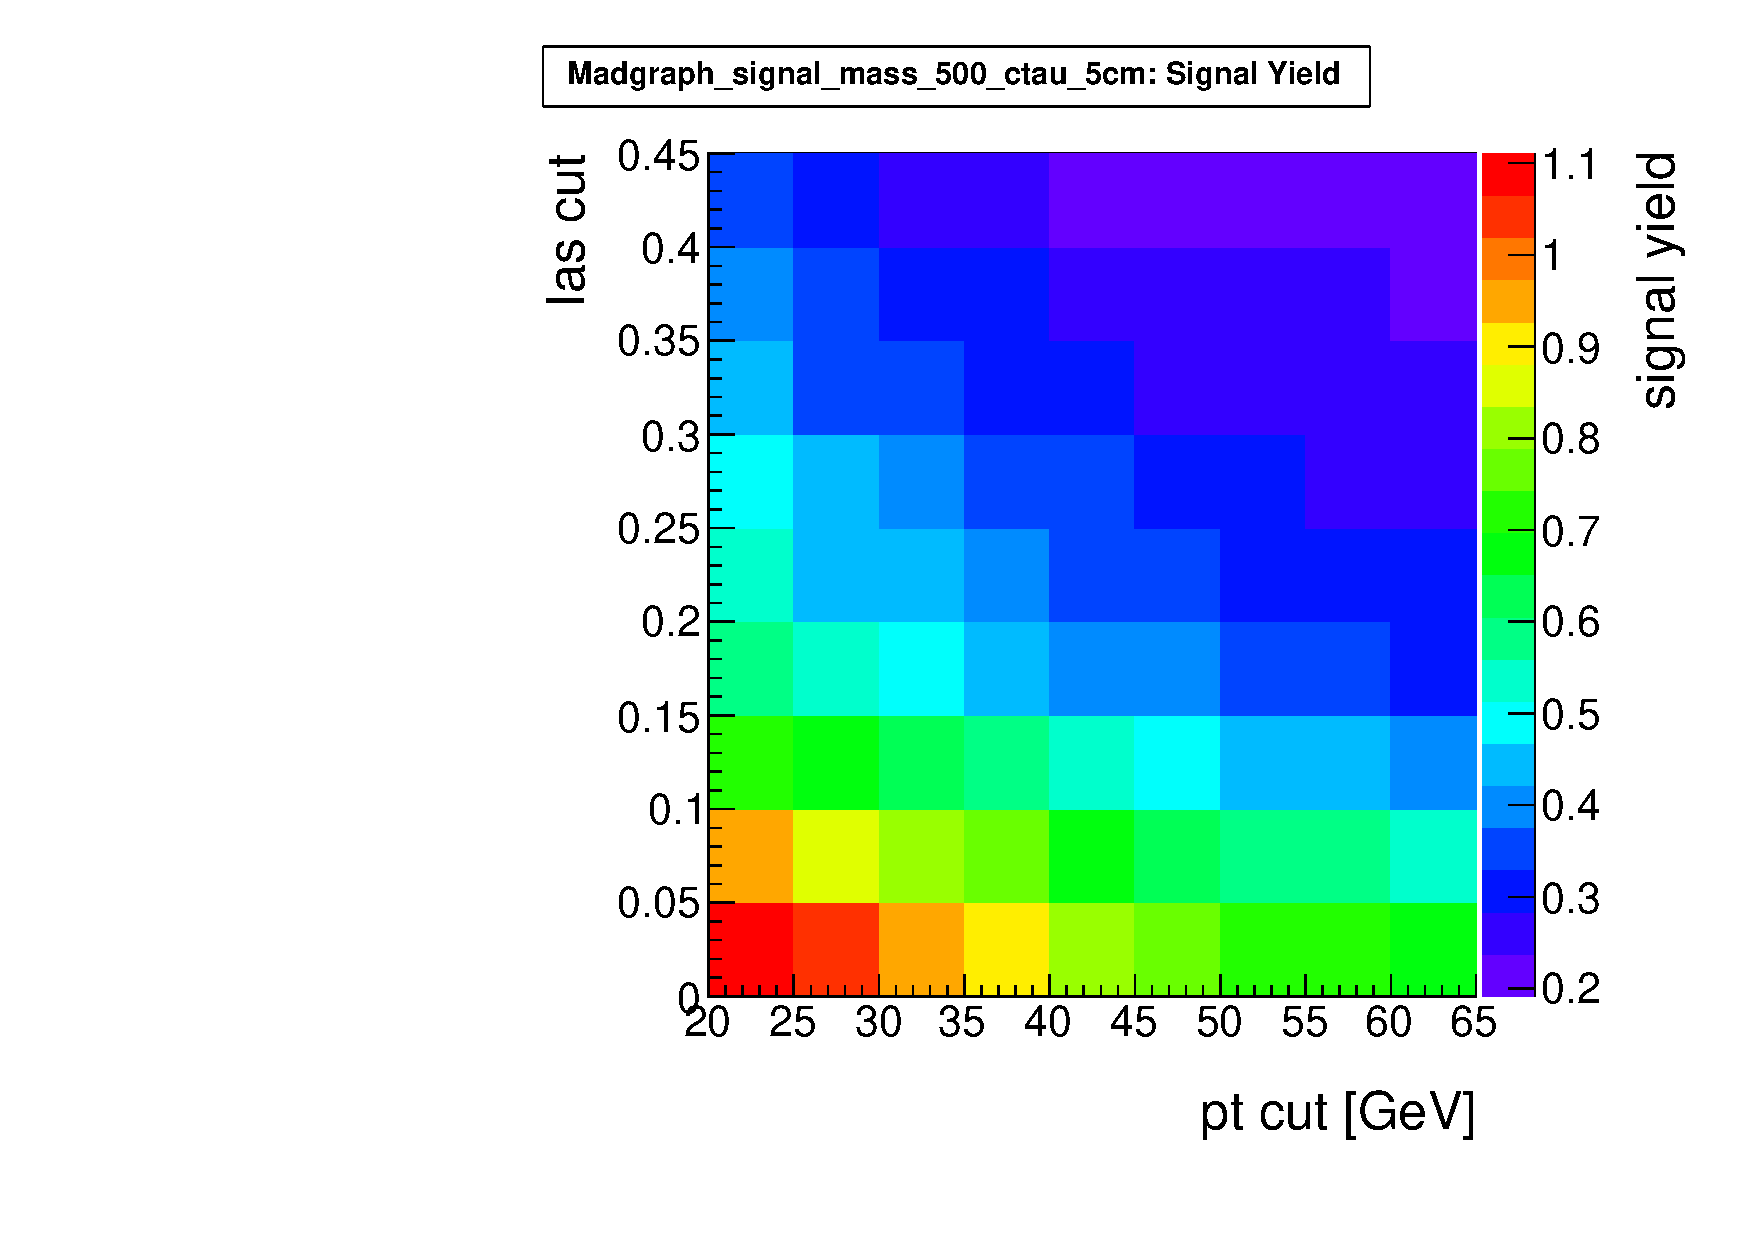
\includegraphics[width=0.35\textwidth]{figures/analysis/Optimisation/Madgraph_signal_mass_500_ctau_5cm_ECaloLe5_SignalYield.pdf}
    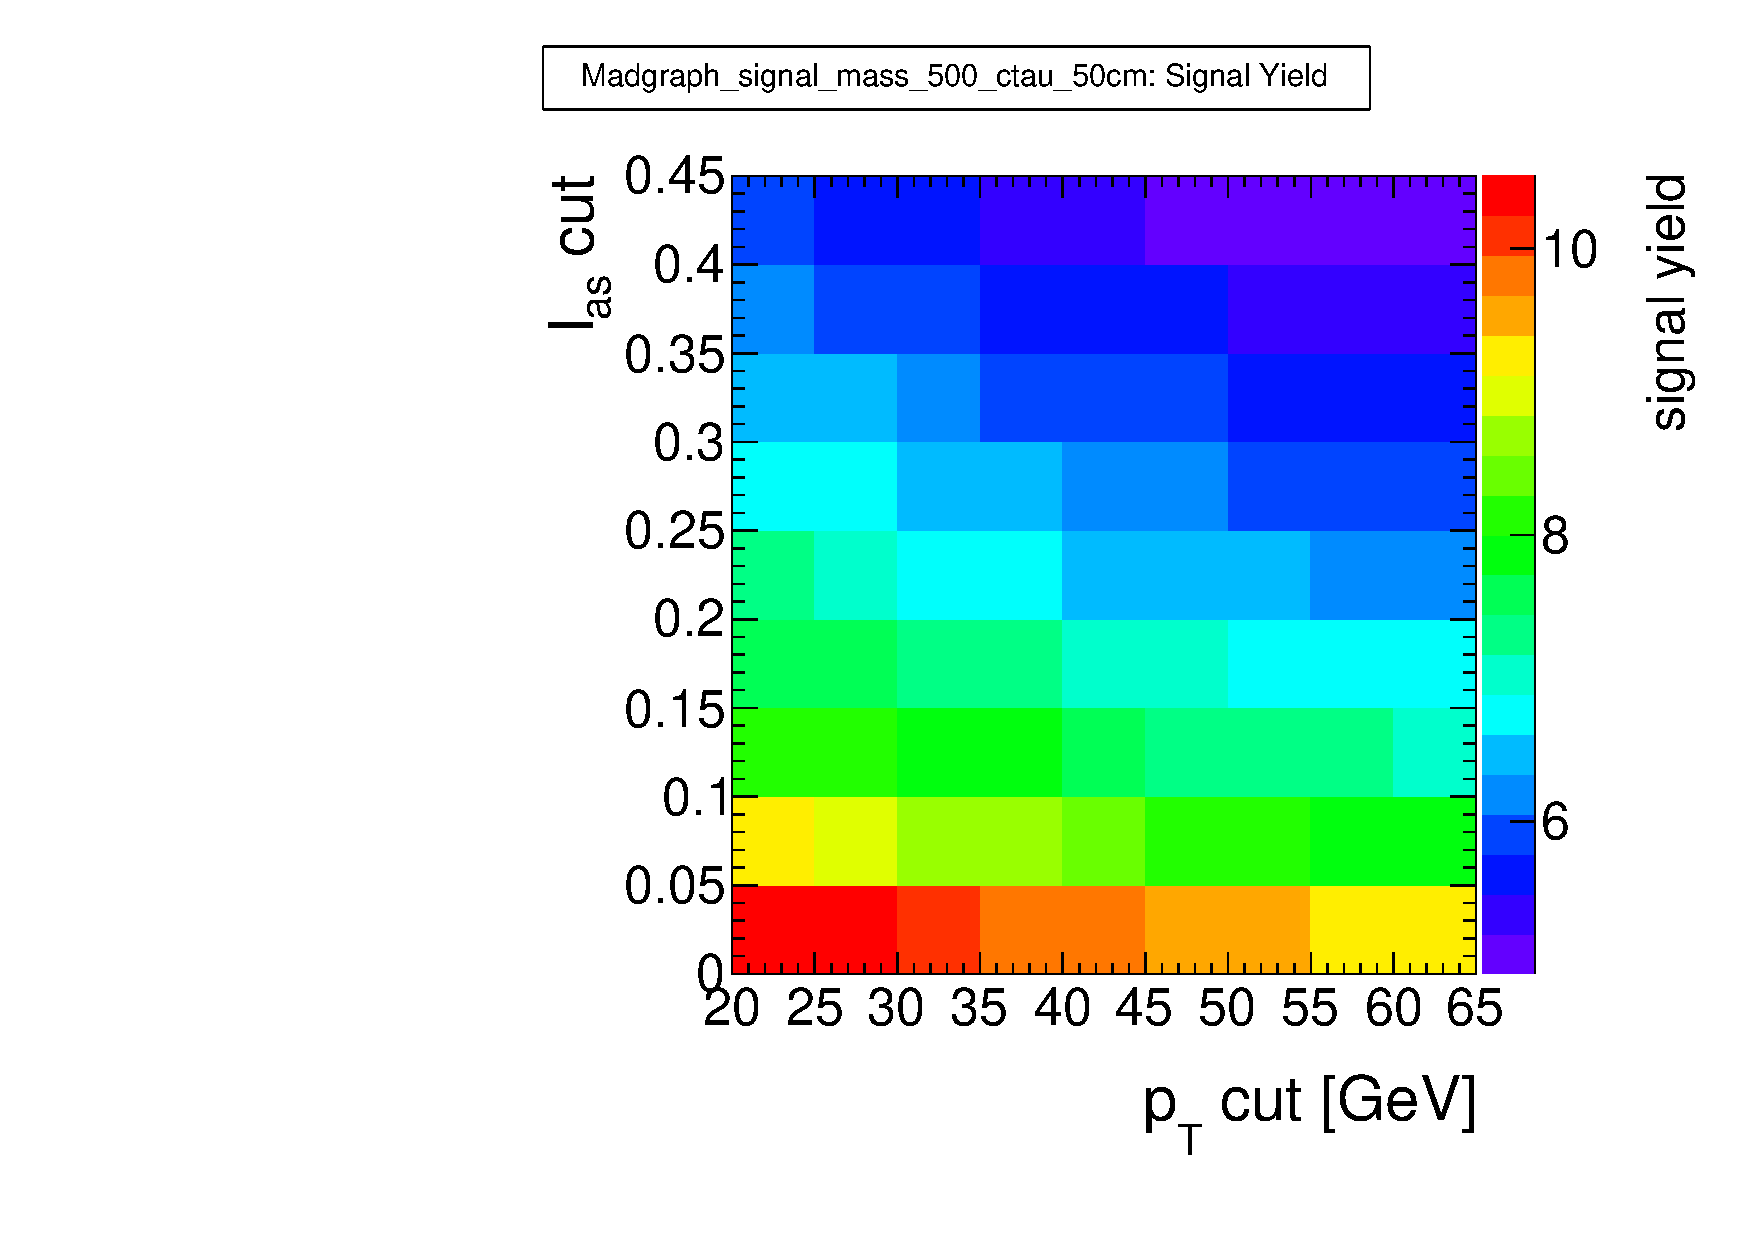
\includegraphics[width=0.35\textwidth]{figures/analysis/Optimisation/Madgraph_signal_mass_500_ctau_50cm_ECaloLe5_SignalYield.pdf}\\ 
  \end{tabular}
  \caption{Background yield, background uncertainty and signal yield for different \pt and \ias selection requirements and four different signal models.}
  \label{fig:optimisationApp}
\end{figure} 


%%%%%%%%%%%%%%%%%%%%%%%%%%%%%%%%%%%%%%%%%%%%%%%%%%%%%%%%%%%%%%%%%%%%%%%%%%%%%%%%%%%%%%%%%%%%%%%%%%%%%%%%%%%%%%%%%%%%%%%%%%%%%%%%%%%%%%%%%%%%%%%%%%%%%%%%%%%%%%%%%%%%%%%
%%%%%%%%%%%%%%%%%%%%%%%%%%%%%%%%%%%%%%%%%%%%%%%%%%%%%%%%%%%%%%%%%%%%%%%%%%%%%%%%%%%%%%%%%%%%%%%%%%%%%%%%%%%%%%%%%%%%%%%%%%%%%%%%%%%%%%%%%%%%%%%%%%%%%%%%%%%%%%%%%%%%%%%
\clearpage
\chapter{Trigger emulation}
\label{app:TriggerEmulation}

As the HLTMonoCentralPFJet80\_PFMETnoMu105\_NHEF0p95 trigger is not availabale in the simulated signal samples, this trigger is emulated in these samples.
Since HLT trigger information is stored in the samples, it is possible to rebuild the trigger afterwards. 

The following requirements must be fulfilled in order to consider the trigger fireing~\cite{bib:CMS:DT_Thesis,bib:CMS:DT_8TeV_AN}:
\begin{itemize}
\item \pt of hltL1sL1ETM40 $>40\gev$
\item \pt of hltCentralJet65L1FastJet $>65\gev$
\item \pt of hltMET65 $>65\gev$
\item \pt of hltCentralPFJet80 $>80\gev$
\item \pt of hltPFMETWOM95 $>105\gev$
\end{itemize}
As a cross check, also the HLTMonoCentralPFJet80\_PFMETnoMu95\_NHEF0p95 is rebuild with the looser selection of \pt of hltPFMETWOM95 $>95\gev$.
The correct implementation could be verified with this test.

%%%%%%%%%%%%%%%%%%%%%%%%%%%%%%%%%%%%%%%%%%%%%%%%%%%%%%%%%%%%%%%%%%%%%%%%%%%%%%%%%%%%%%%%%%%%%%%%%%%%%%%%%%%%%%%%%%%%%%%%%%%%%%%%%%%%%%%%%%%%%%%%%%%%%%%%%%%%%%%%%%%%%%%
%%%%%%%%%%%%%%%%%%%%%%%%%%%%%%%%%%%%%%%%%%%%%%%%%%%%%%%%%%%%%%%%%%%%%%%%%%%%%%%%%%%%%%%%%%%%%%%%%%%%%%%%%%%%%%%%%%%%%%%%%%%%%%%%%%%%%%%%%%%%%%%%%%%%%%%%%%%%%%%%%%%%%%%
\clearpage
\chapter{Exclusion limits for all simulated lifetimes}
\label{app:LimitPlots2d}

\begin{figure}[!h]
  \centering 
  \begin{tabular}{c}
    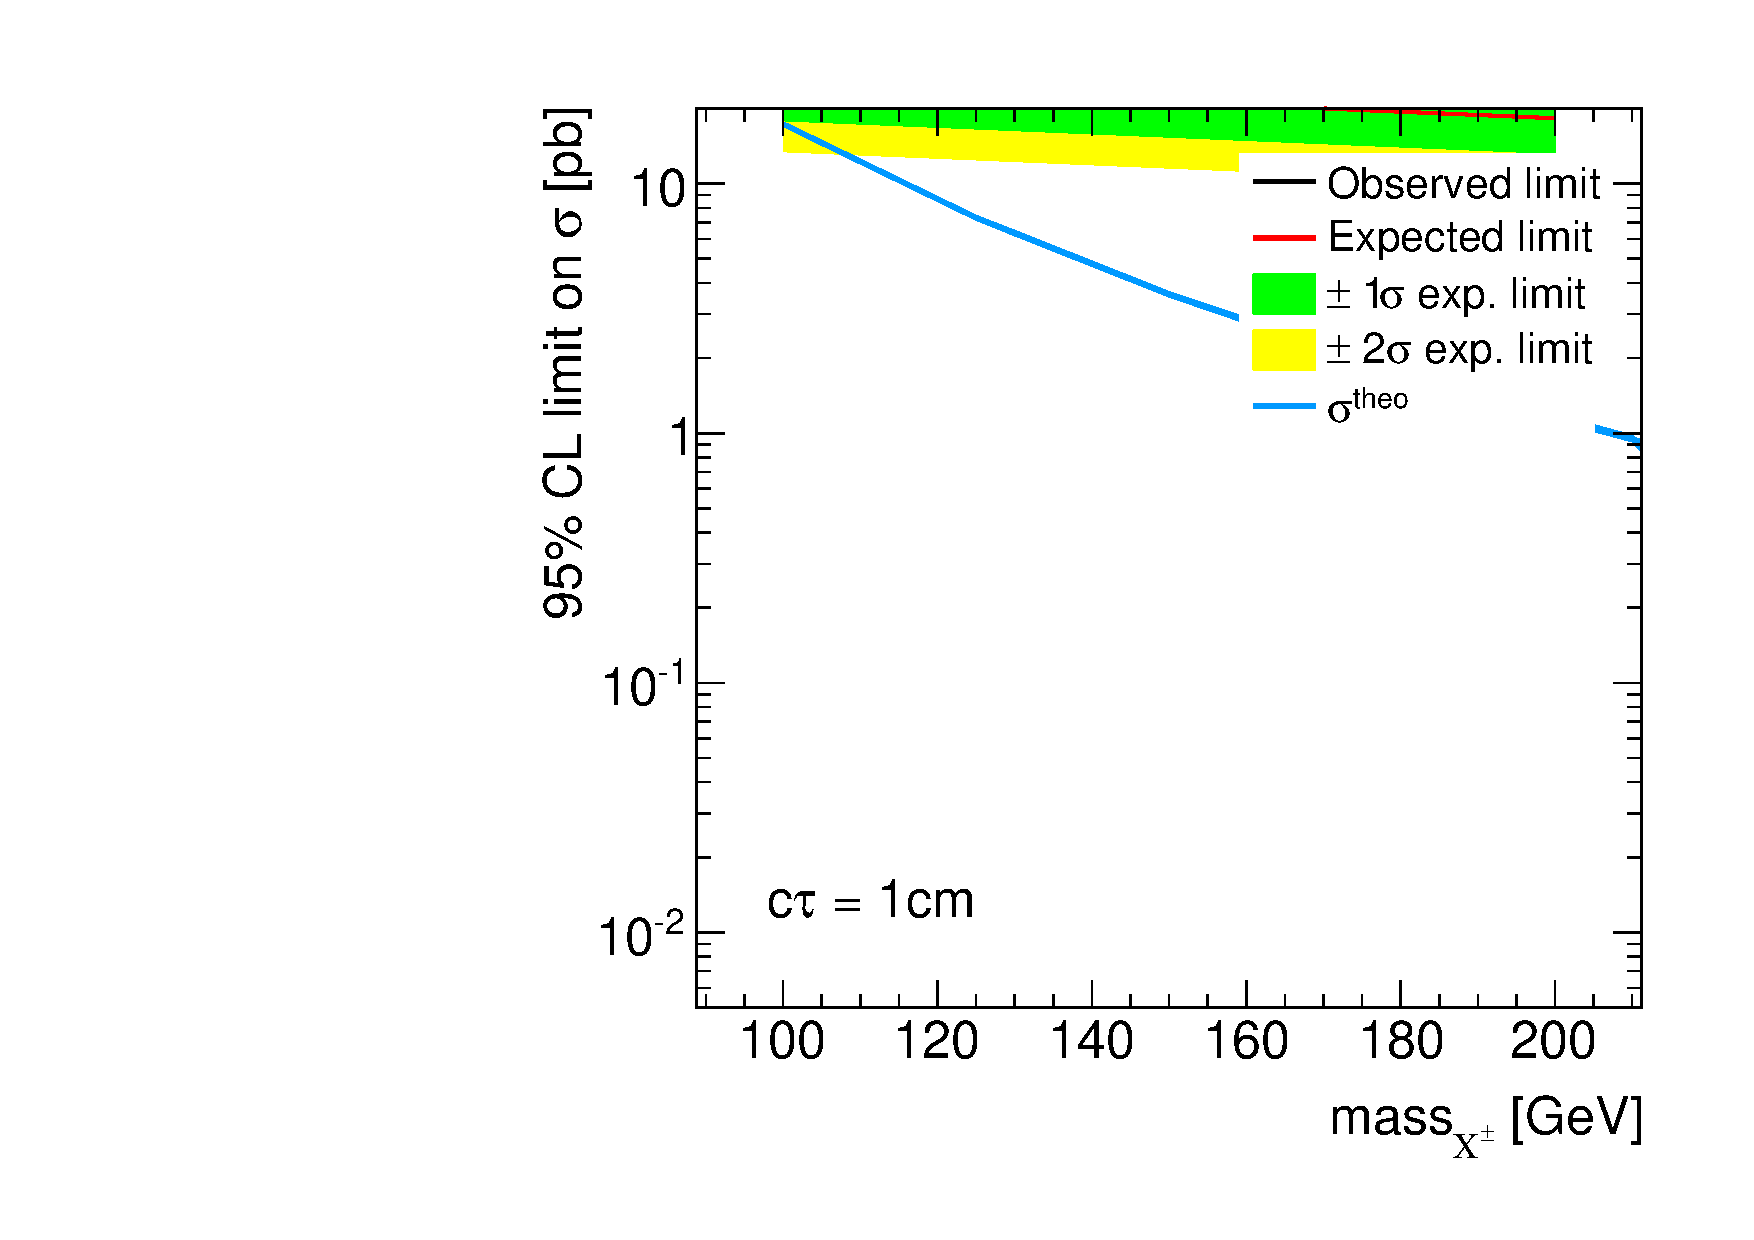
\includegraphics[width=0.29\textwidth]{figures/analysis/Interpretation/ExclusionLimits/LimitPlot_ctau1cm.pdf} 
    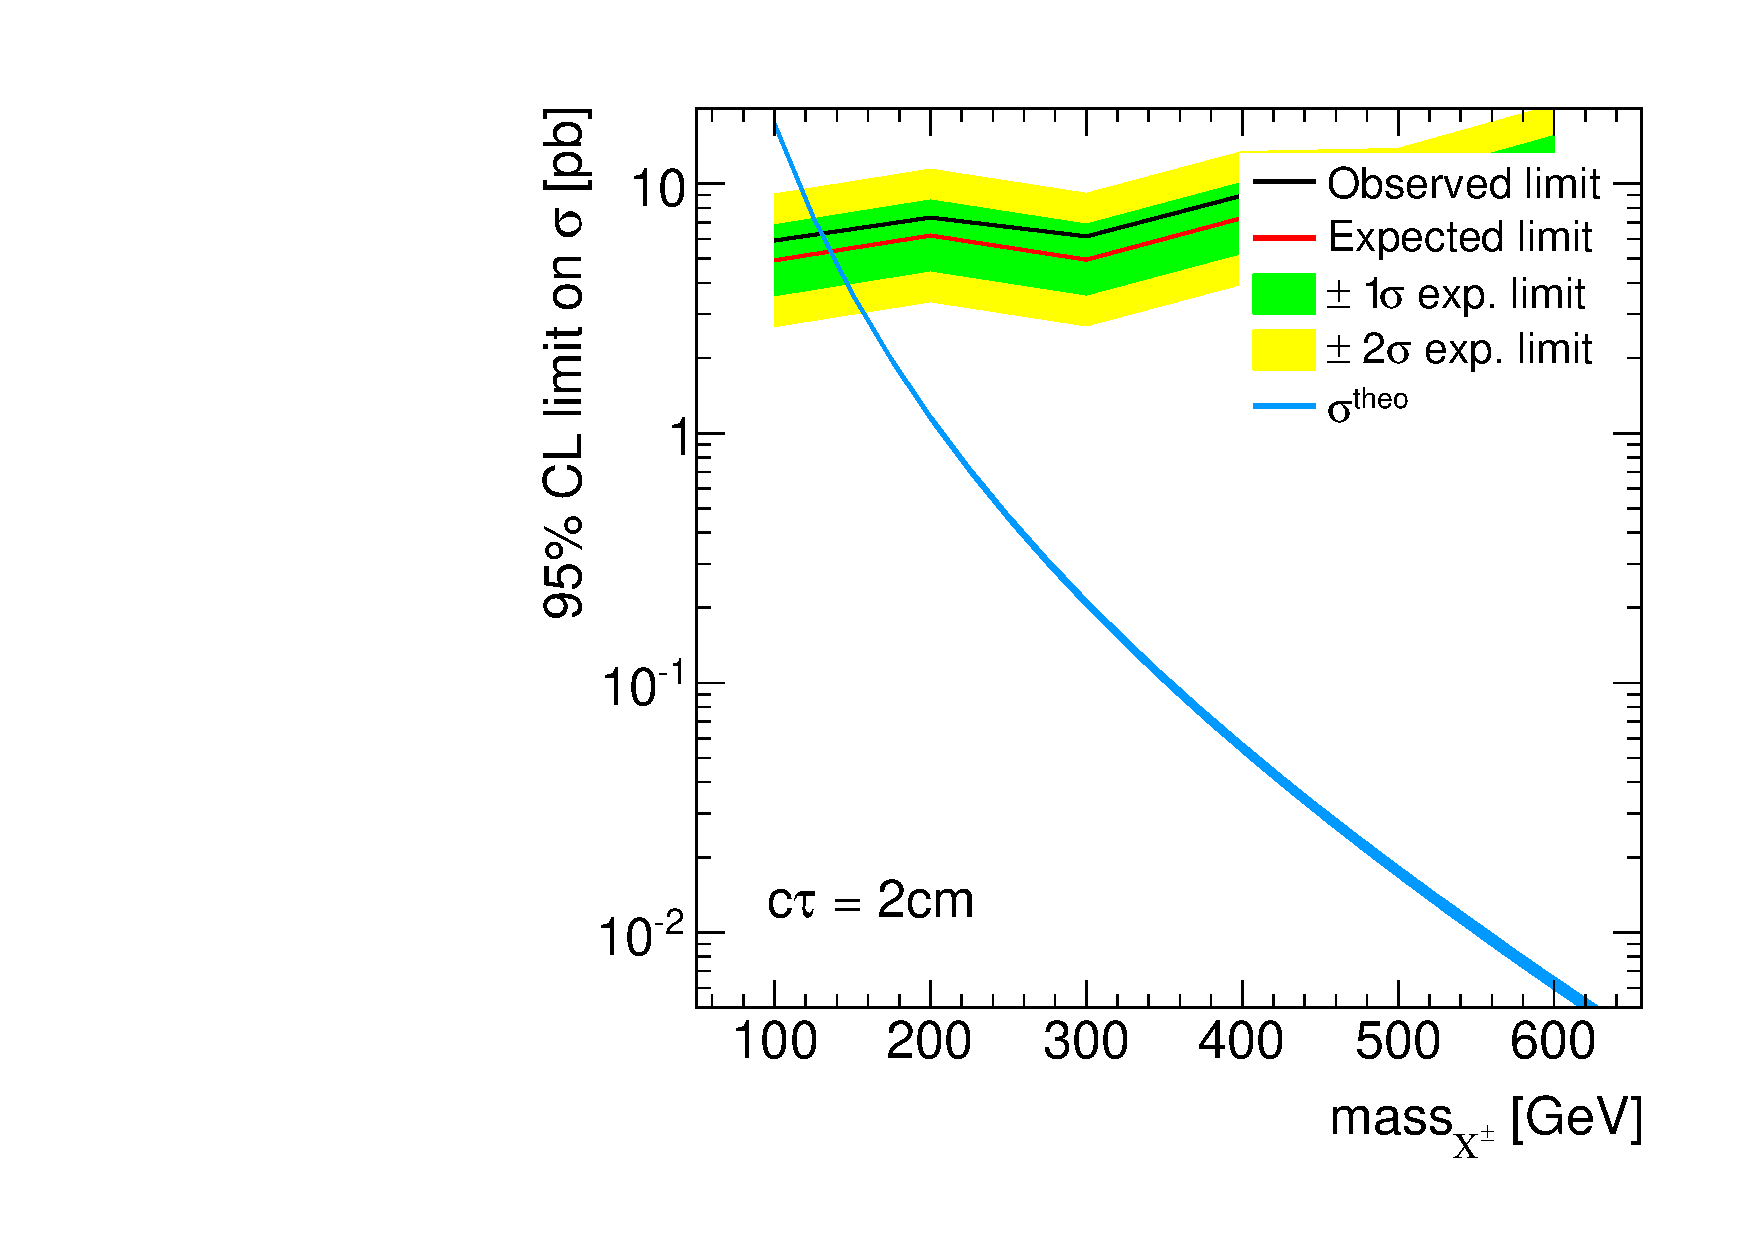
\includegraphics[width=0.29\textwidth]{figures/analysis/Interpretation/ExclusionLimits/LimitPlot_ctau2cm.pdf} 
    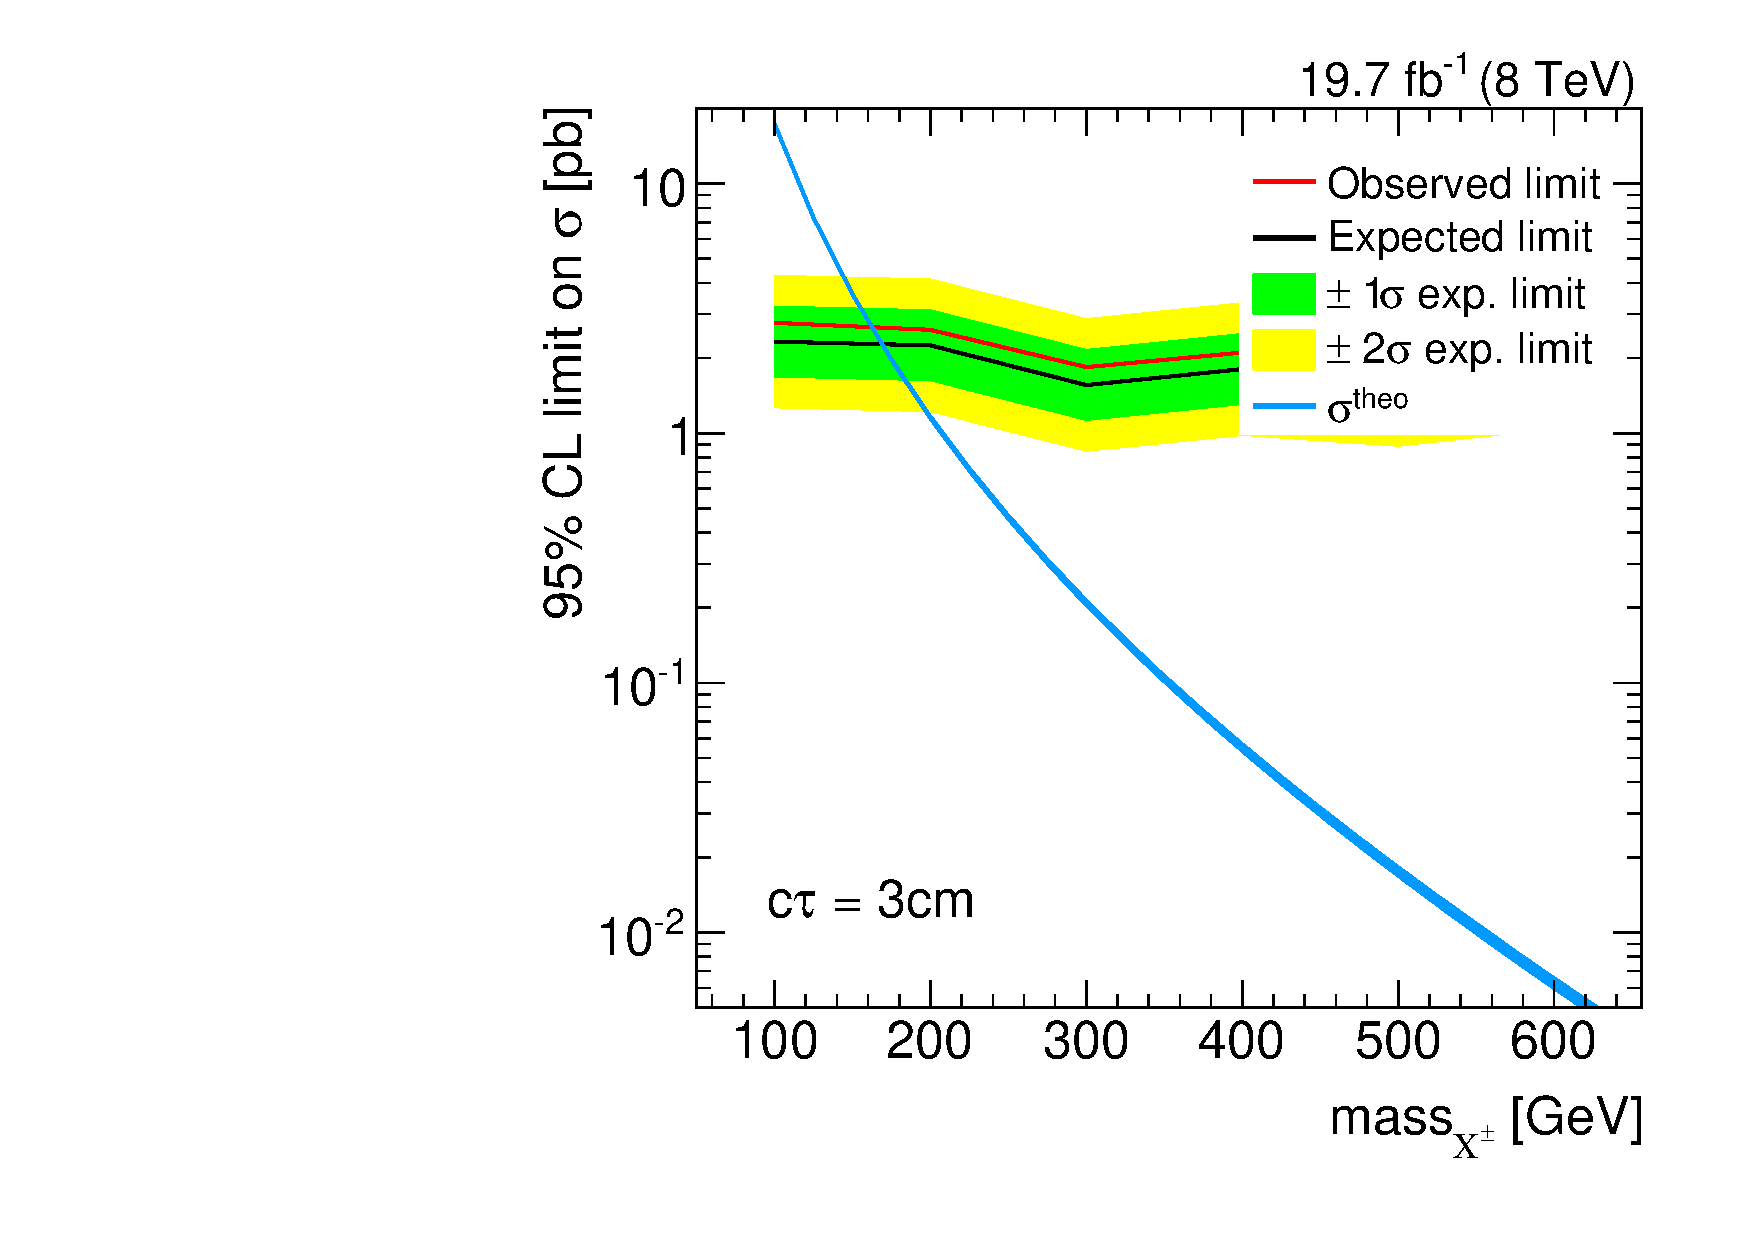
\includegraphics[width=0.29\textwidth]{figures/analysis/Interpretation/ExclusionLimits/LimitPlot_ctau3cm.pdf} \\
    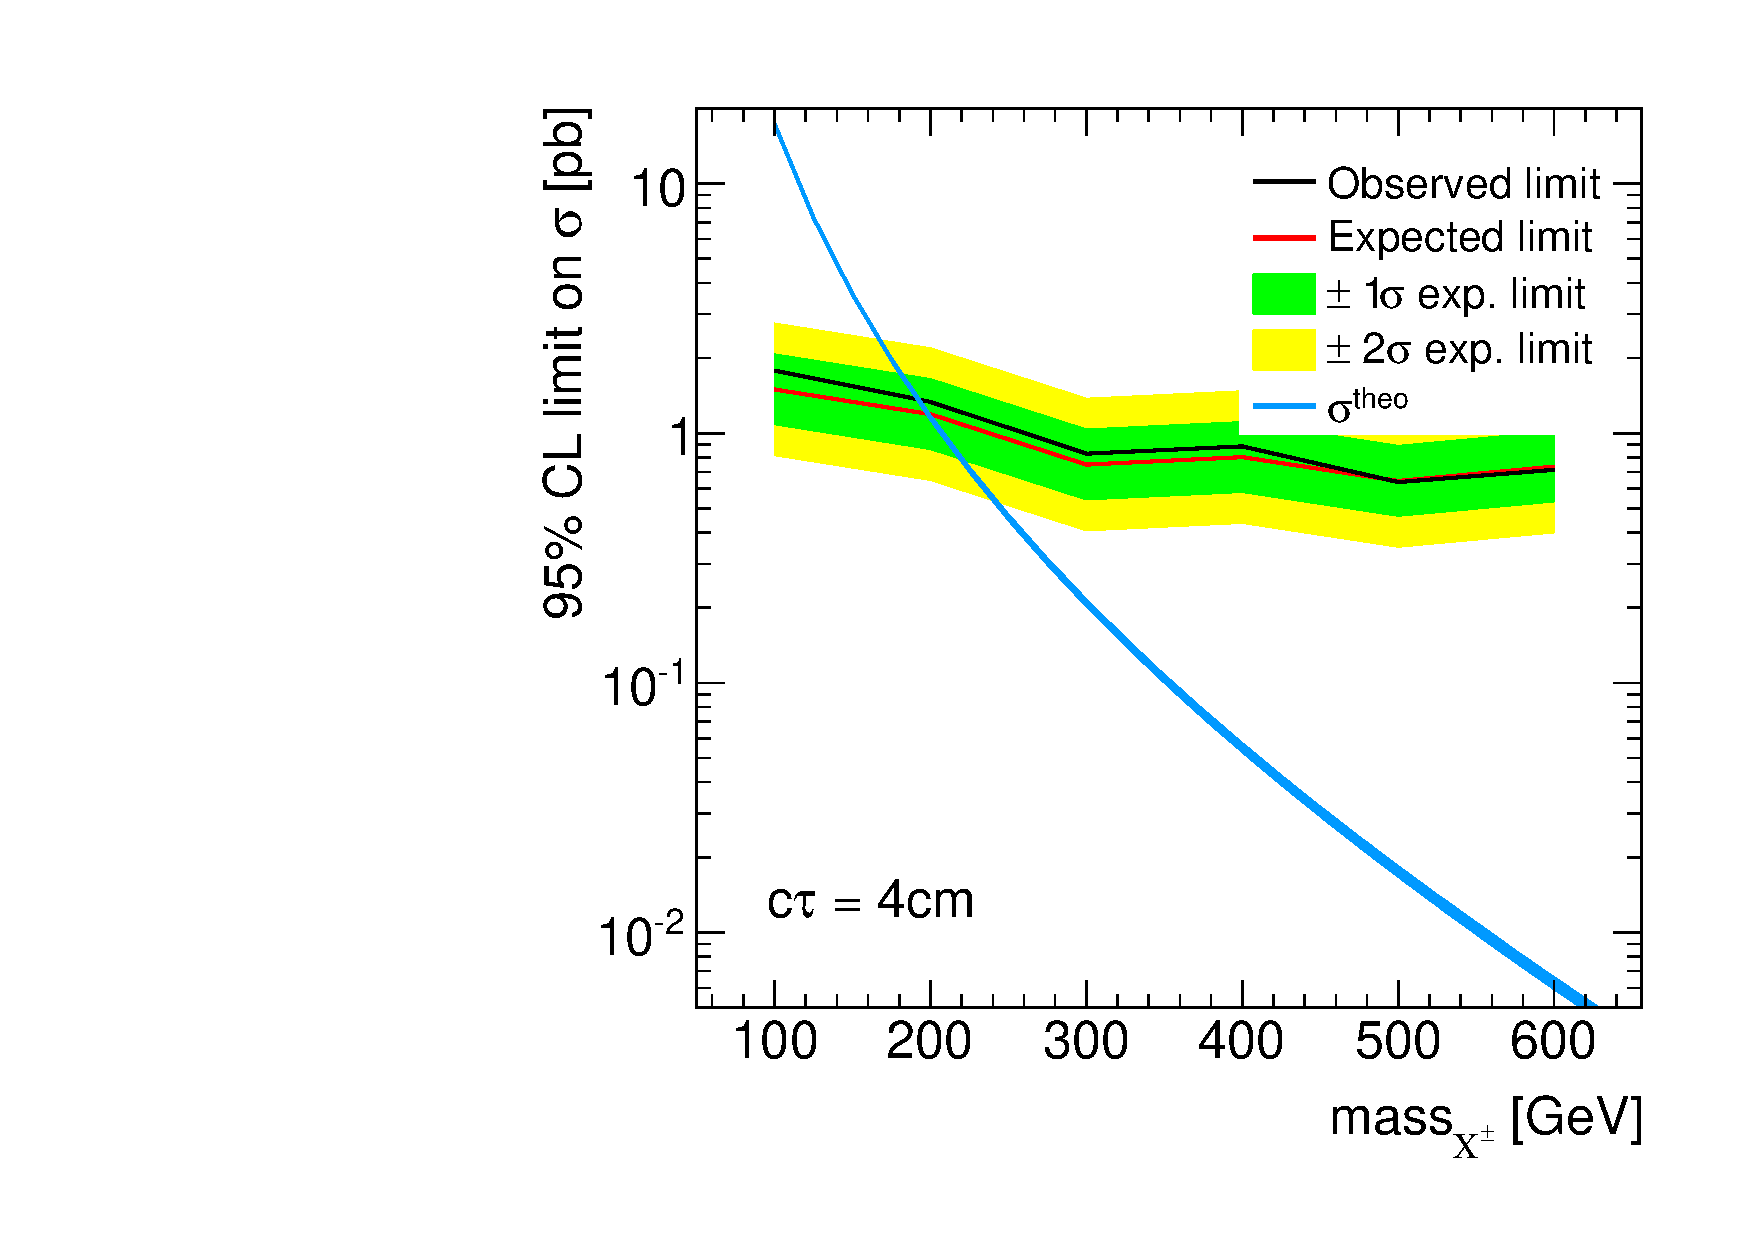
\includegraphics[width=0.29\textwidth]{figures/analysis/Interpretation/ExclusionLimits/LimitPlot_ctau4cm.pdf} 
    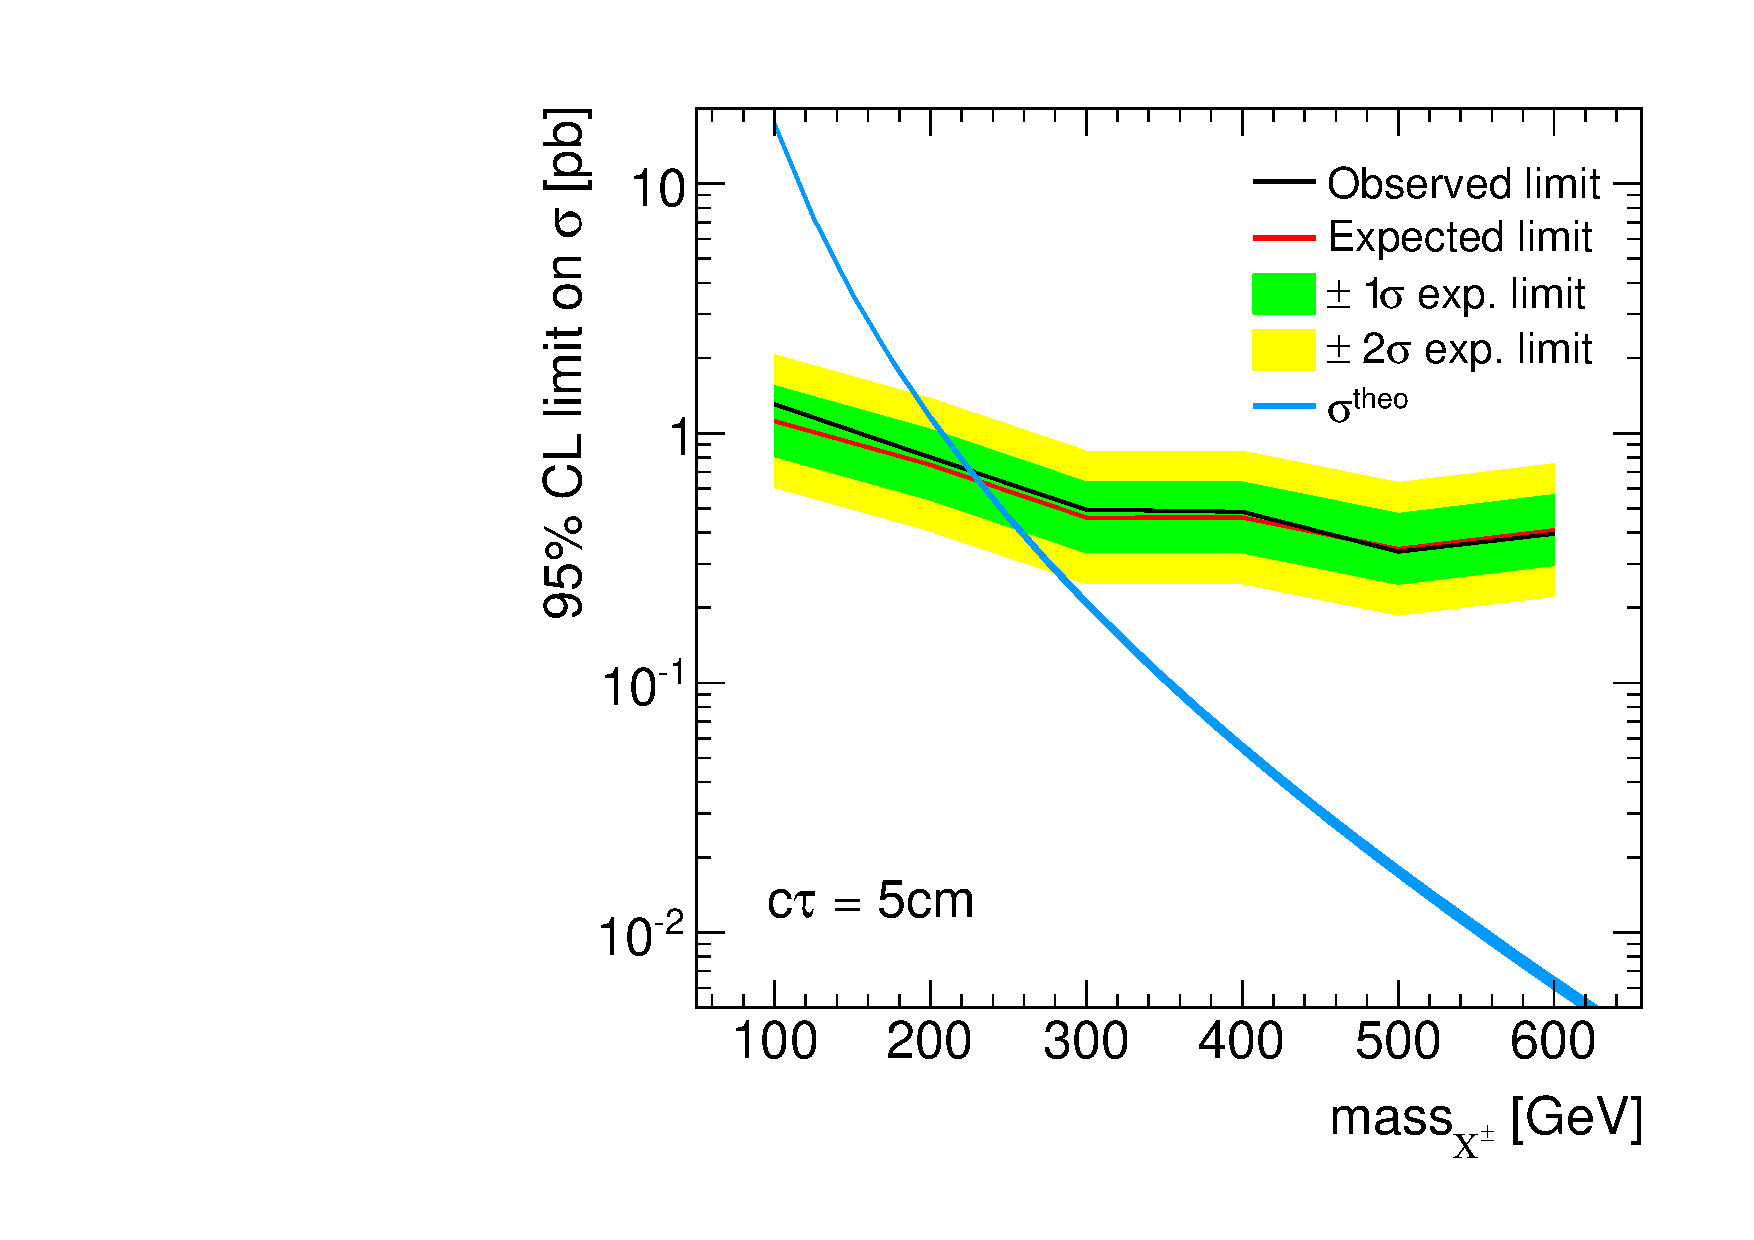
\includegraphics[width=0.29\textwidth]{figures/analysis/Interpretation/ExclusionLimits/LimitPlot_ctau5cm.pdf} 
    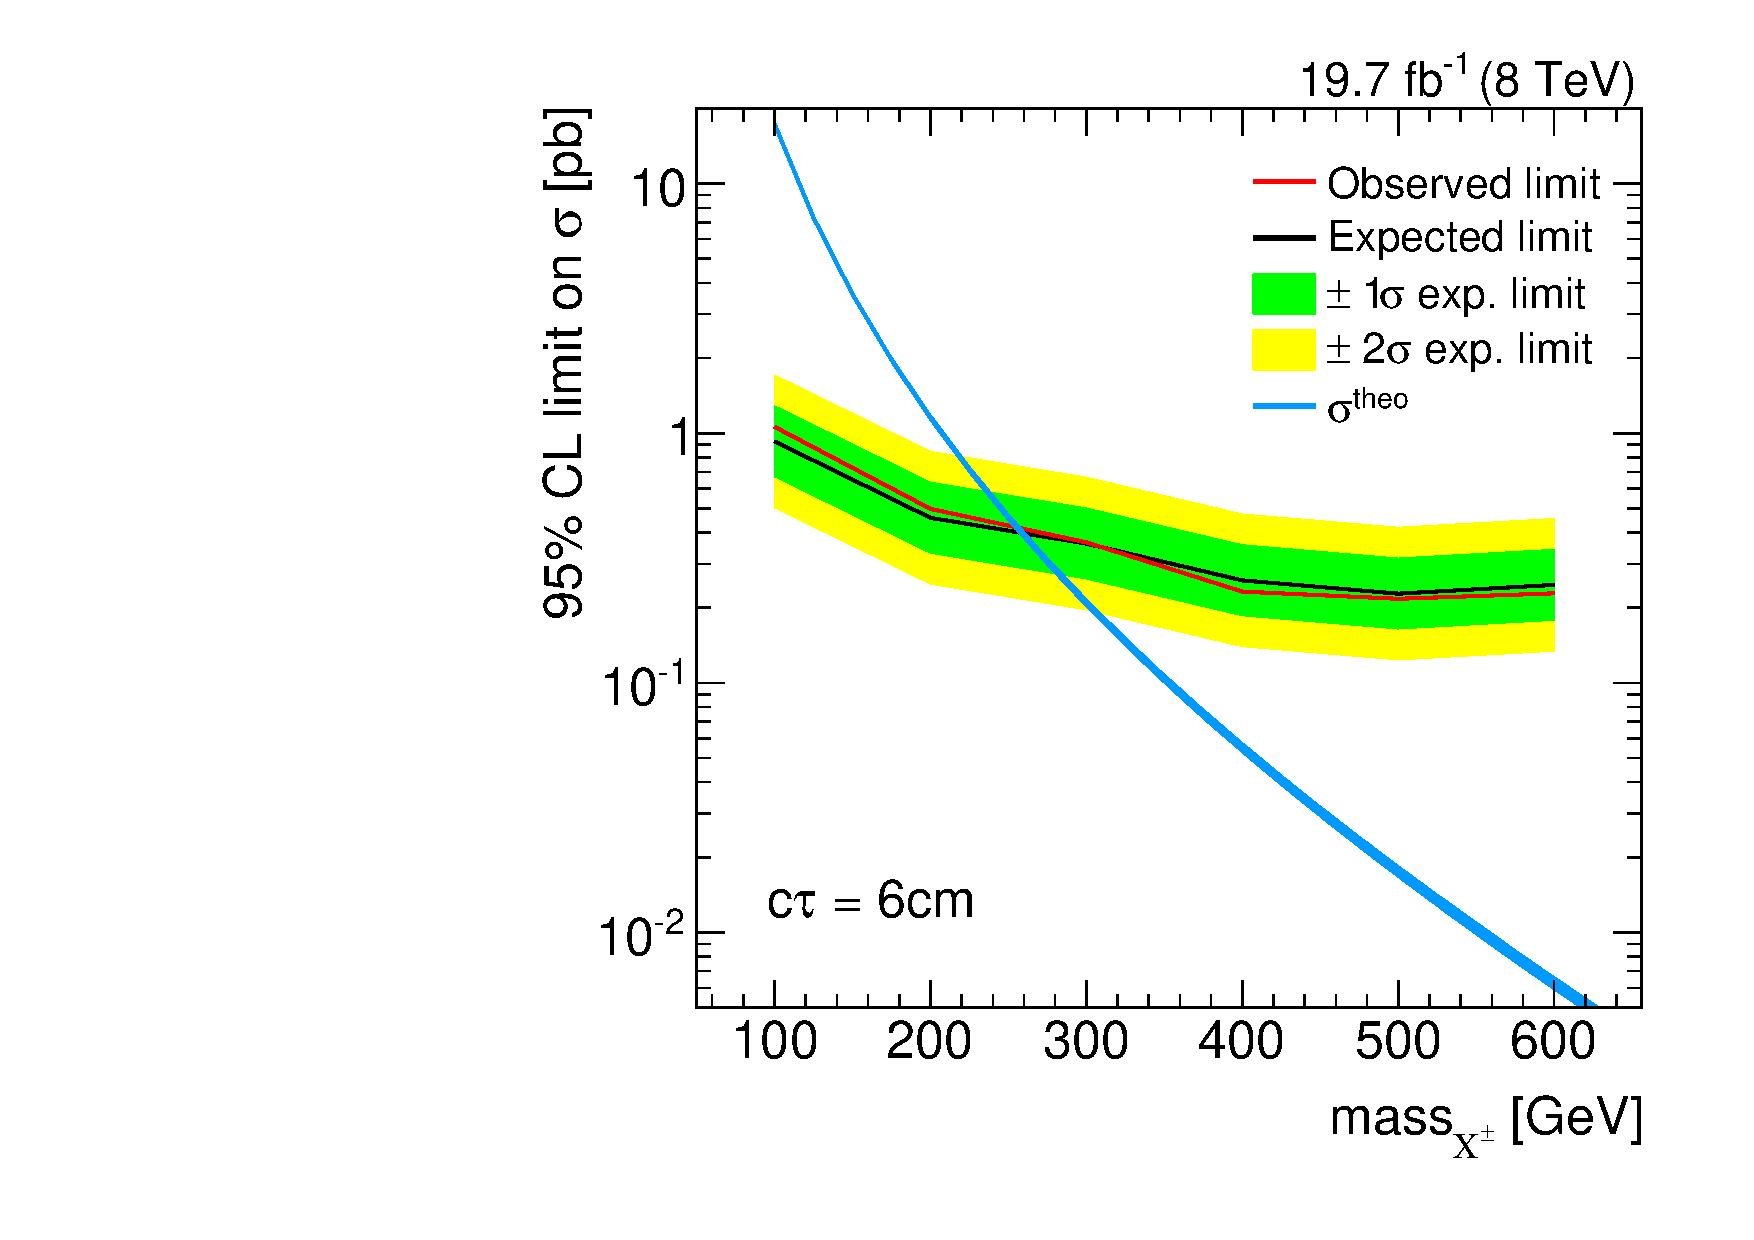
\includegraphics[width=0.29\textwidth]{figures/analysis/Interpretation/ExclusionLimits/LimitPlot_ctau6cm.pdf} \\
    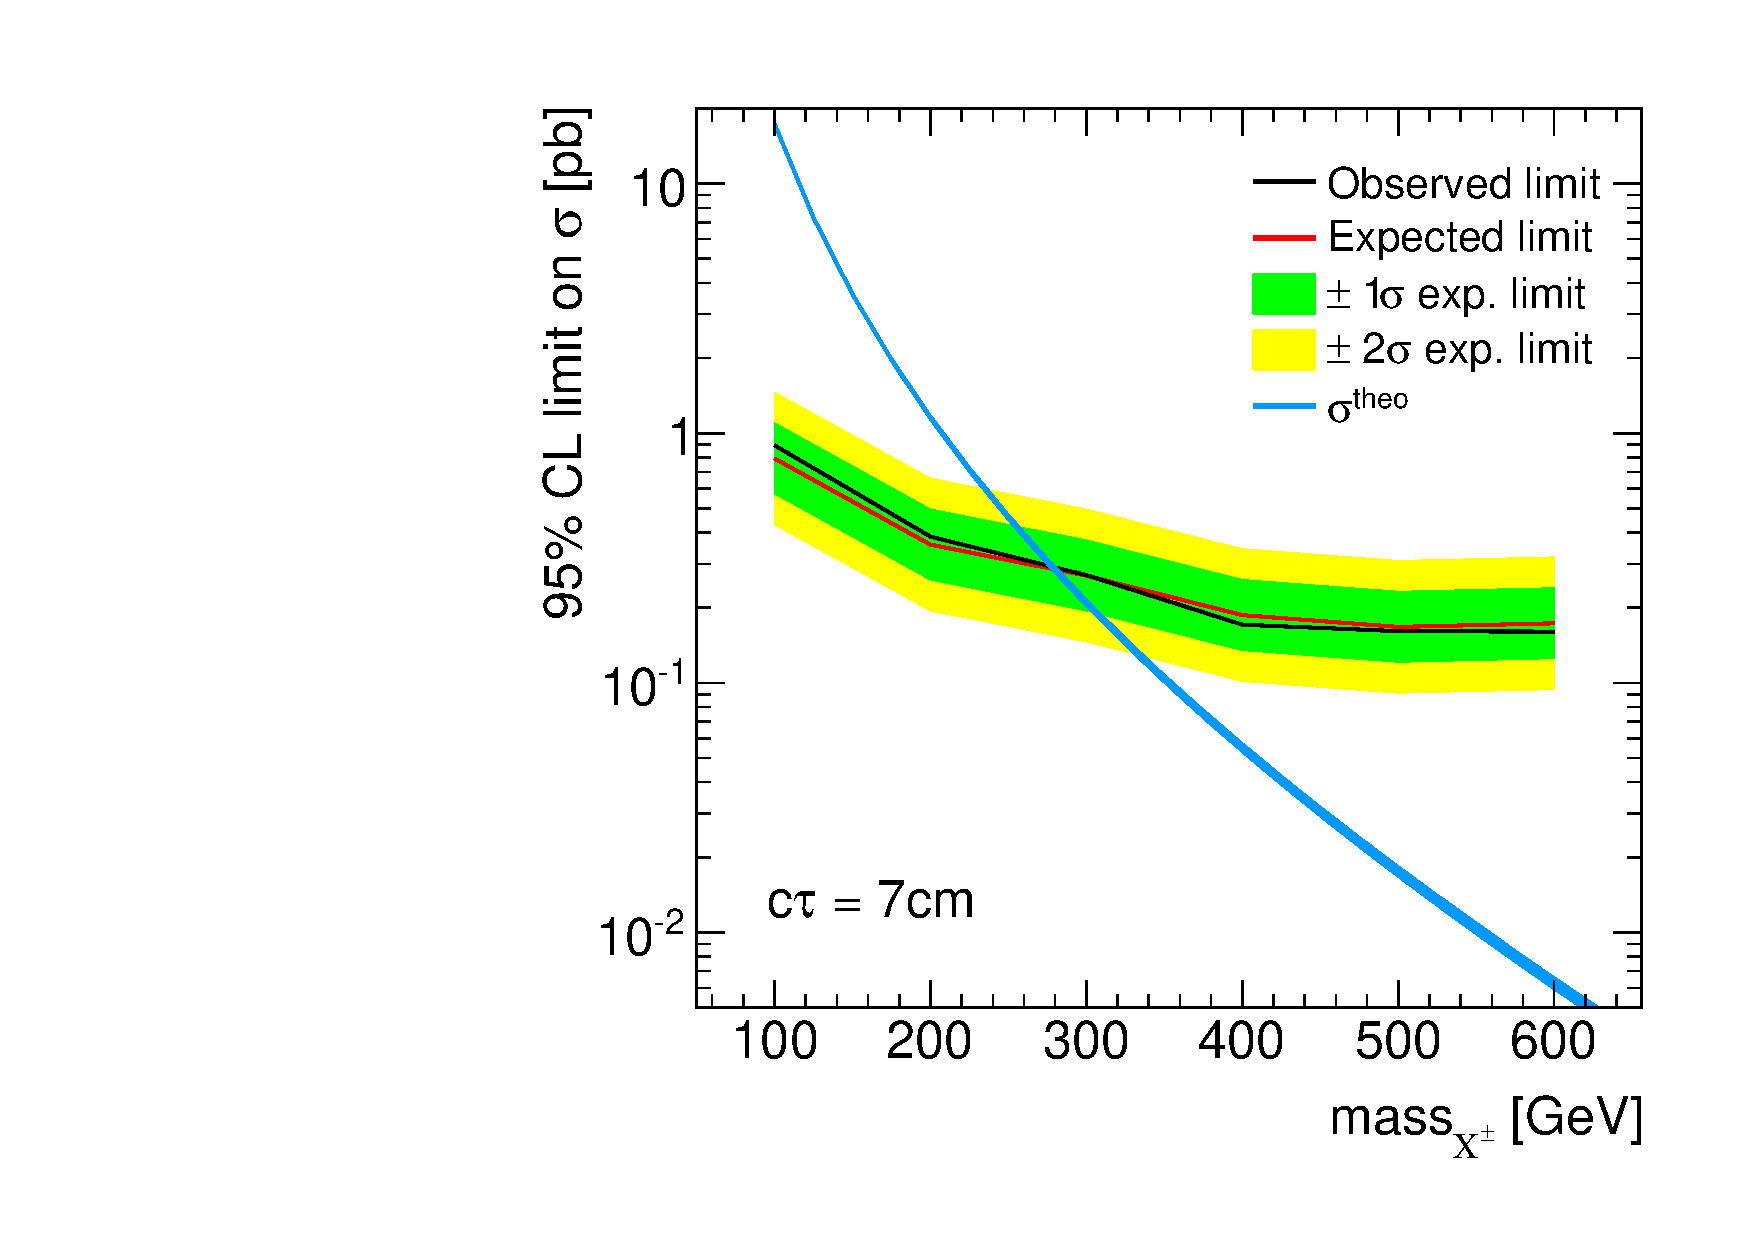
\includegraphics[width=0.29\textwidth]{figures/analysis/Interpretation/ExclusionLimits/LimitPlot_ctau7cm.pdf} 
    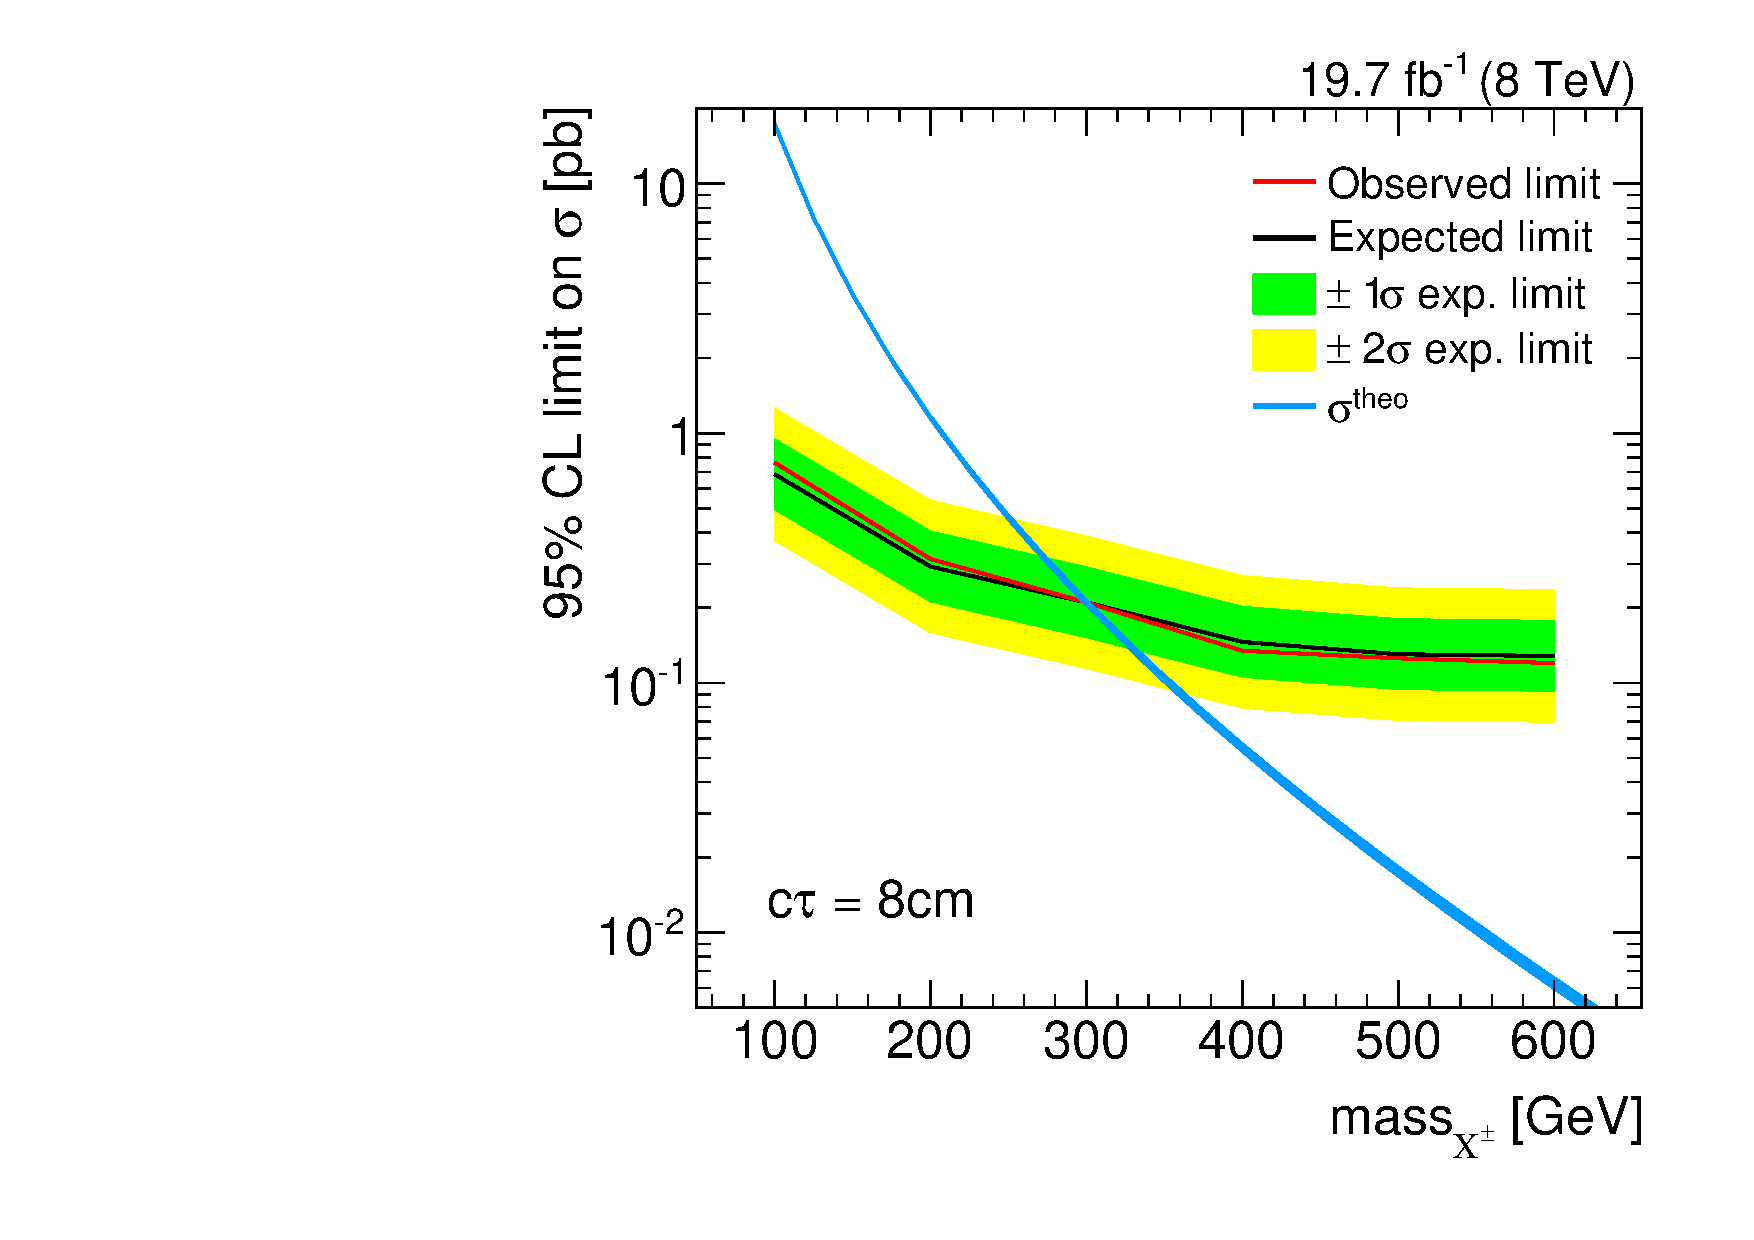
\includegraphics[width=0.29\textwidth]{figures/analysis/Interpretation/ExclusionLimits/LimitPlot_ctau8cm.pdf} 
    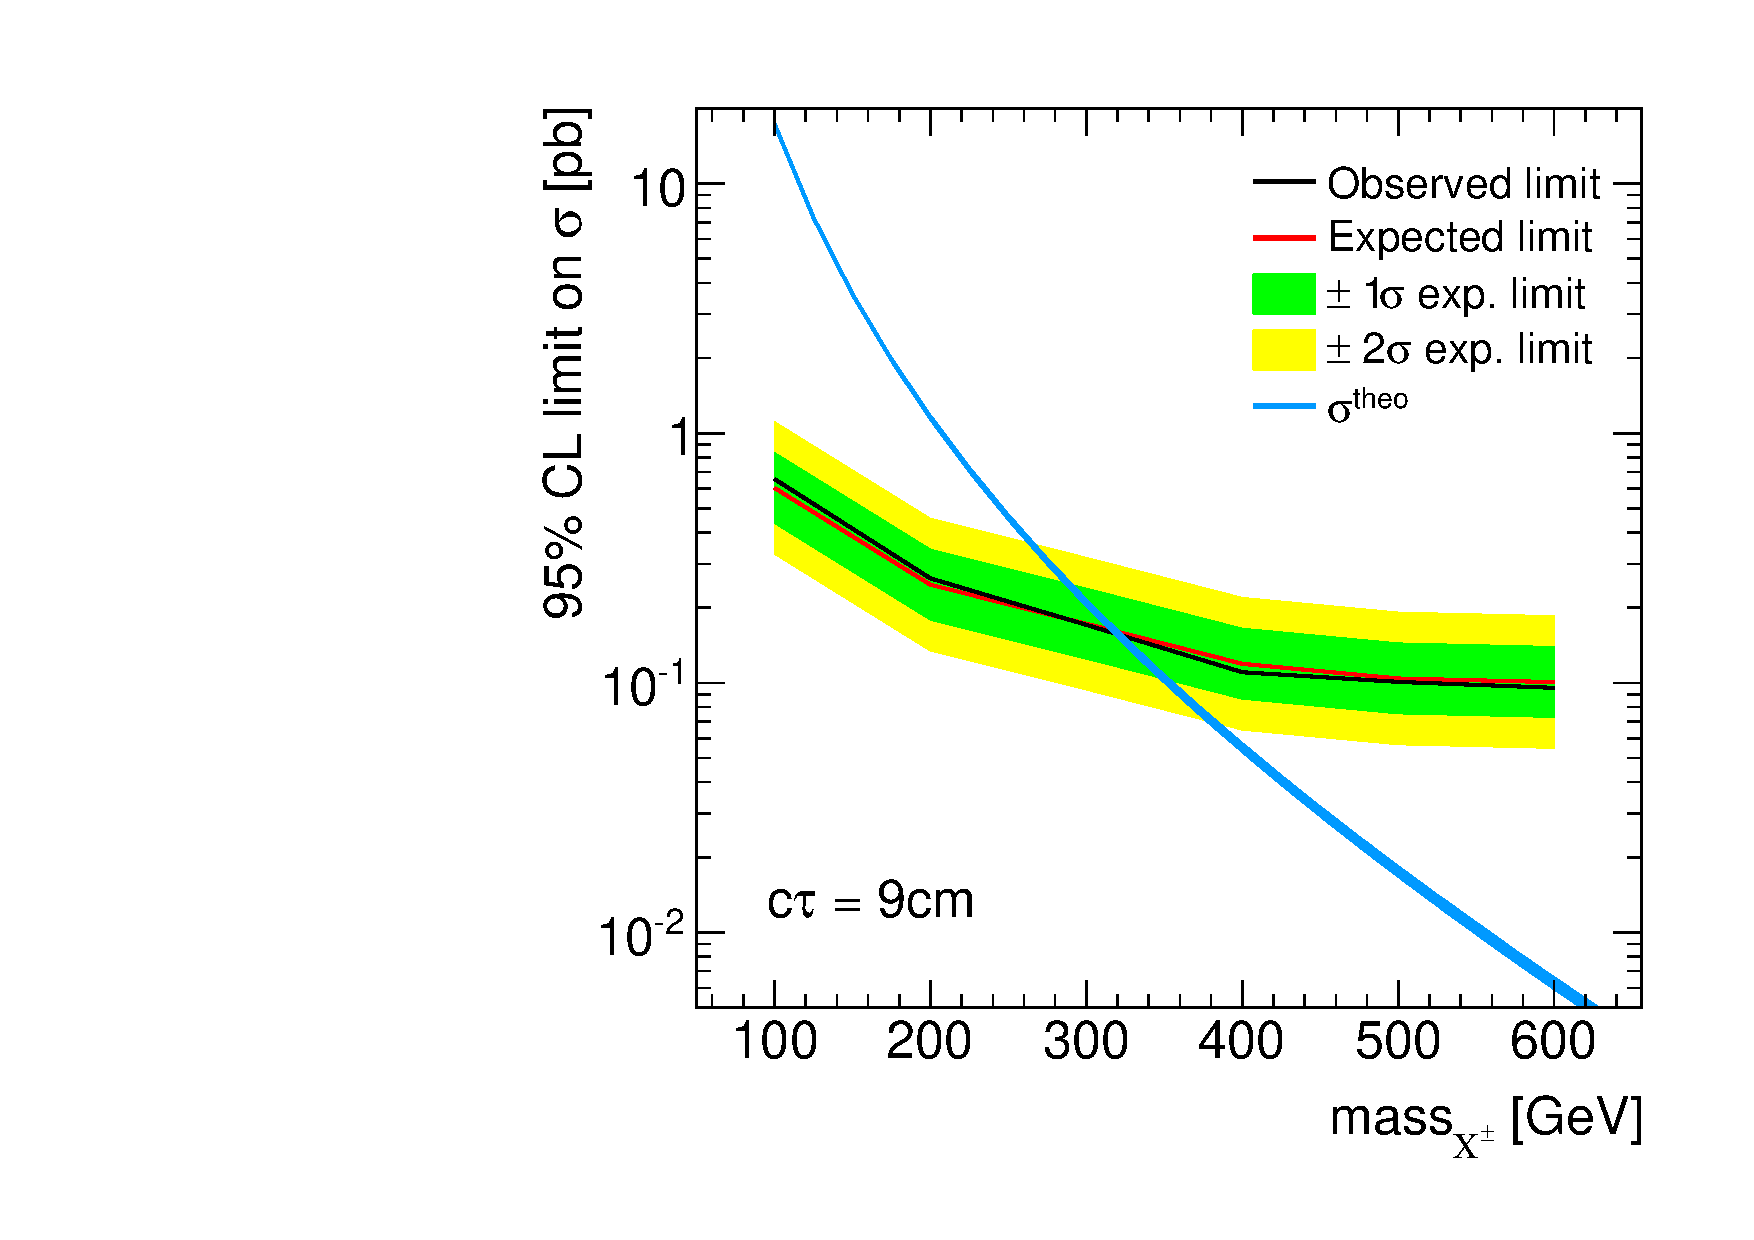
\includegraphics[width=0.29\textwidth]{figures/analysis/Interpretation/ExclusionLimits/LimitPlot_ctau9cm.pdf} \\
    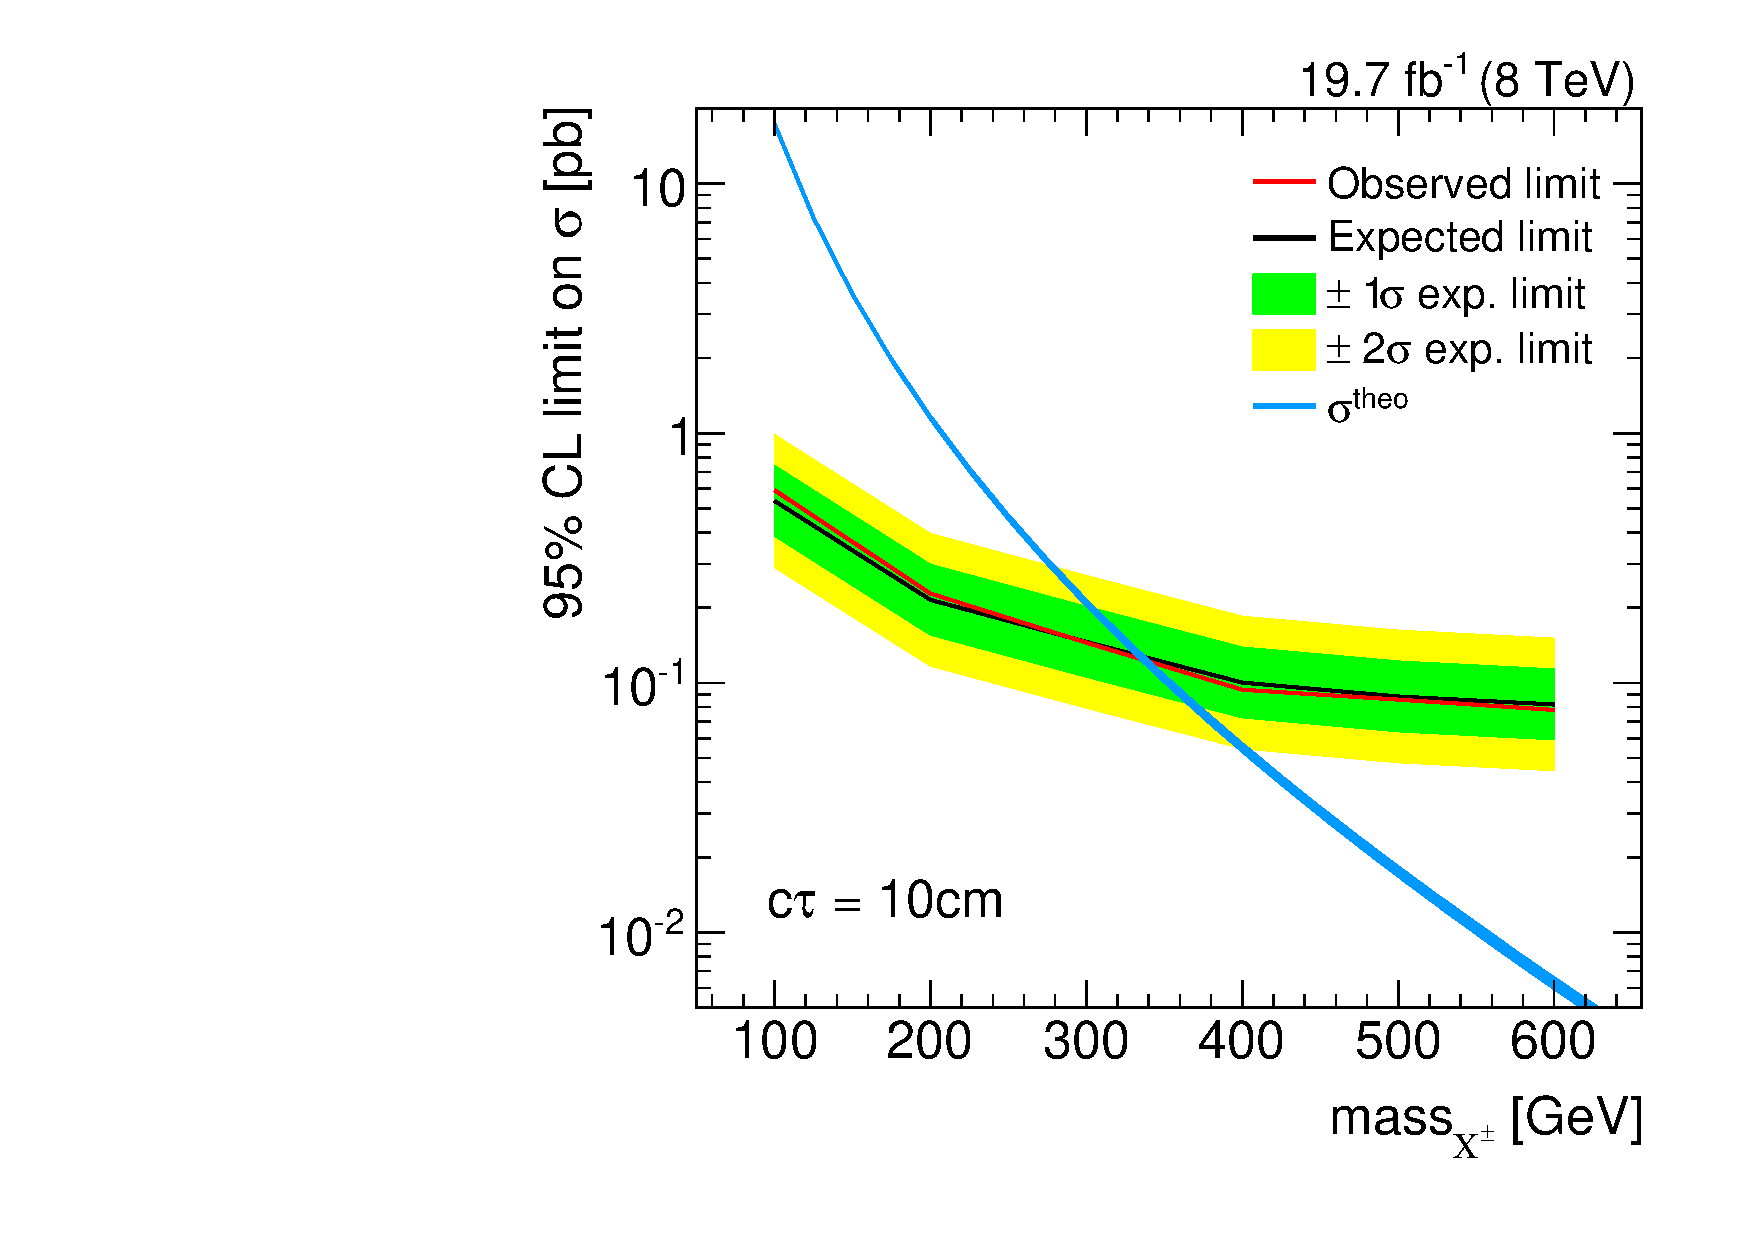
\includegraphics[width=0.29\textwidth]{figures/analysis/Interpretation/ExclusionLimits/LimitPlot_ctau10cm.pdf} 
    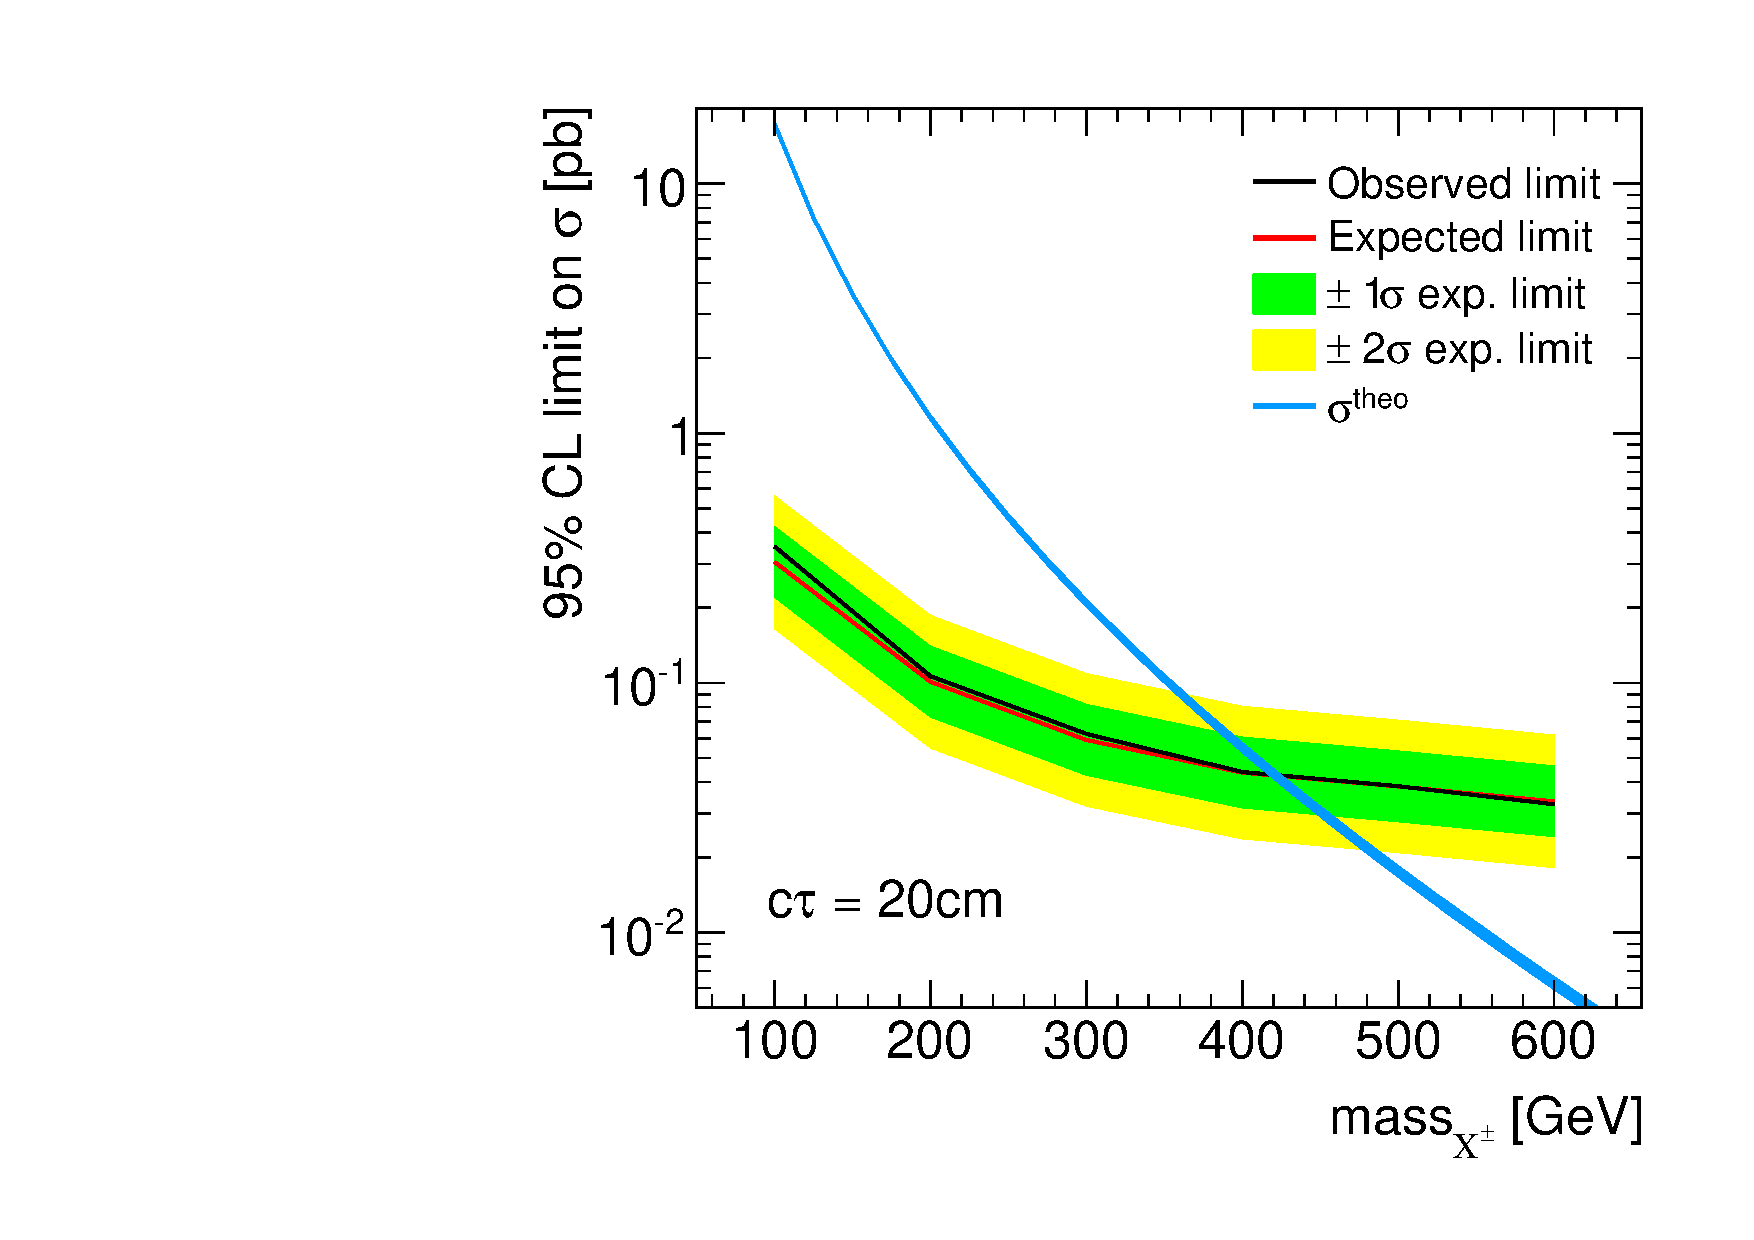
\includegraphics[width=0.29\textwidth]{figures/analysis/Interpretation/ExclusionLimits/LimitPlot_ctau20cm.pdf} 
    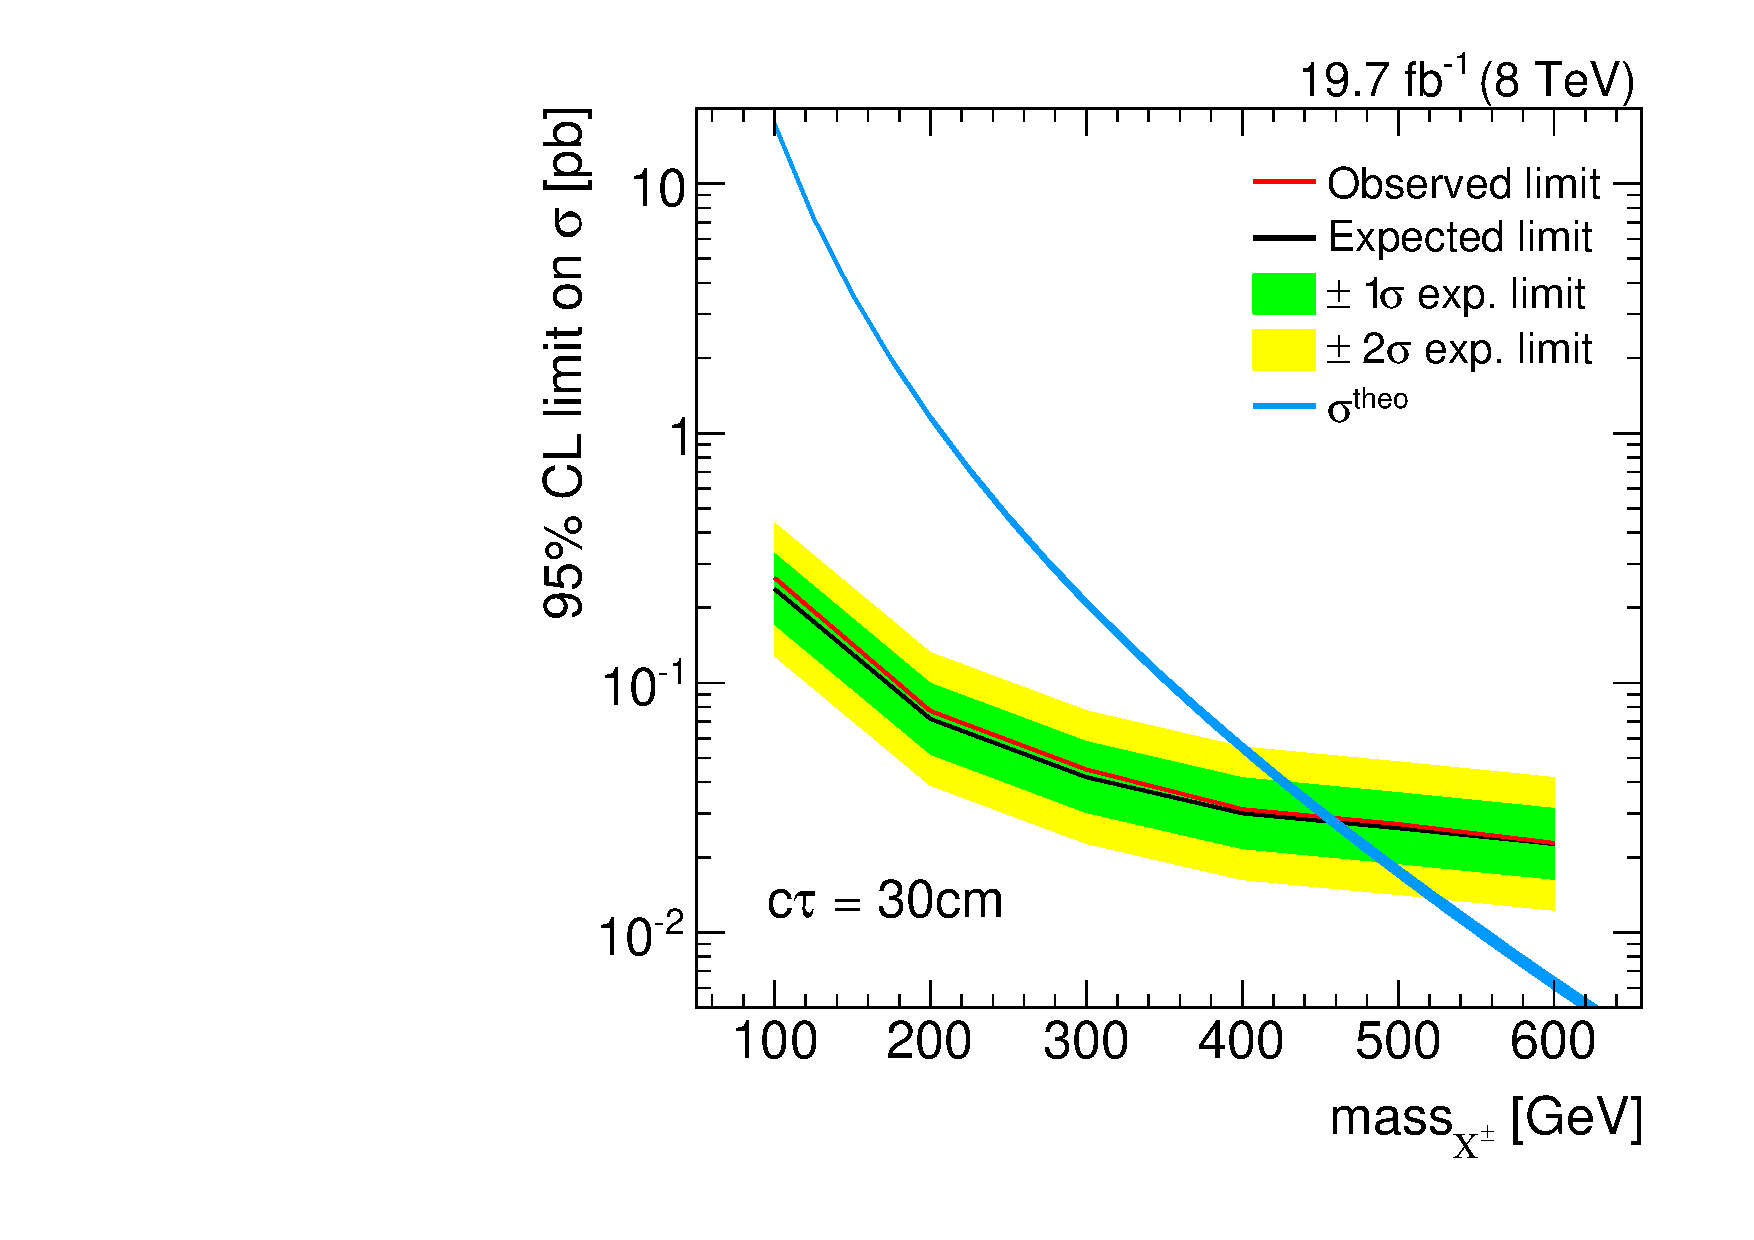
\includegraphics[width=0.29\textwidth]{figures/analysis/Interpretation/ExclusionLimits/LimitPlot_ctau30cm.pdf} \\
  \end{tabular}
  \caption{95\% CL exclusion limits for signal models with $\ctau = 1-30\cm$.}
  \label{fig:1dLimitsA}
\end{figure}

\begin{figure}[!h]
  \centering 
  \begin{tabular}{c}
    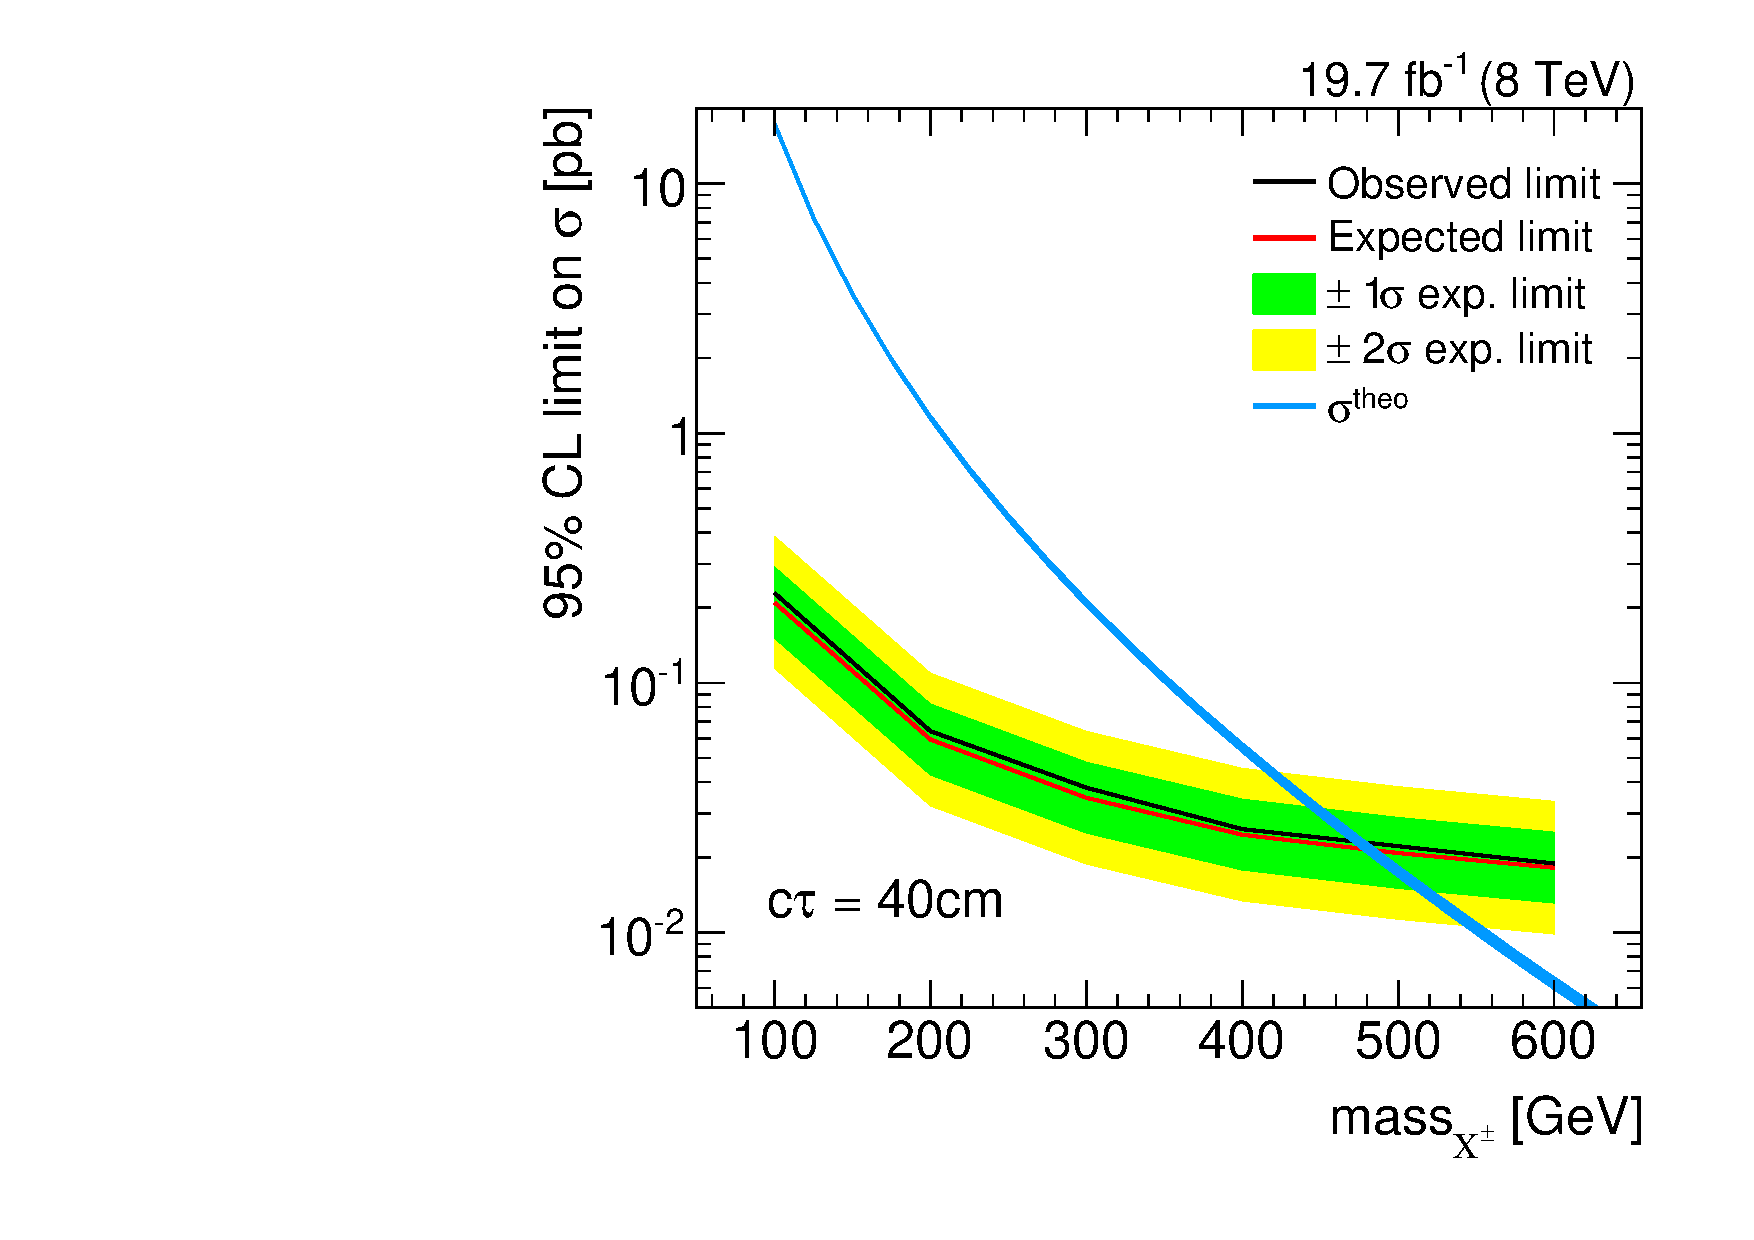
\includegraphics[width=0.29\textwidth]{figures/analysis/Interpretation/ExclusionLimits/LimitPlot_ctau40cm.pdf} 
    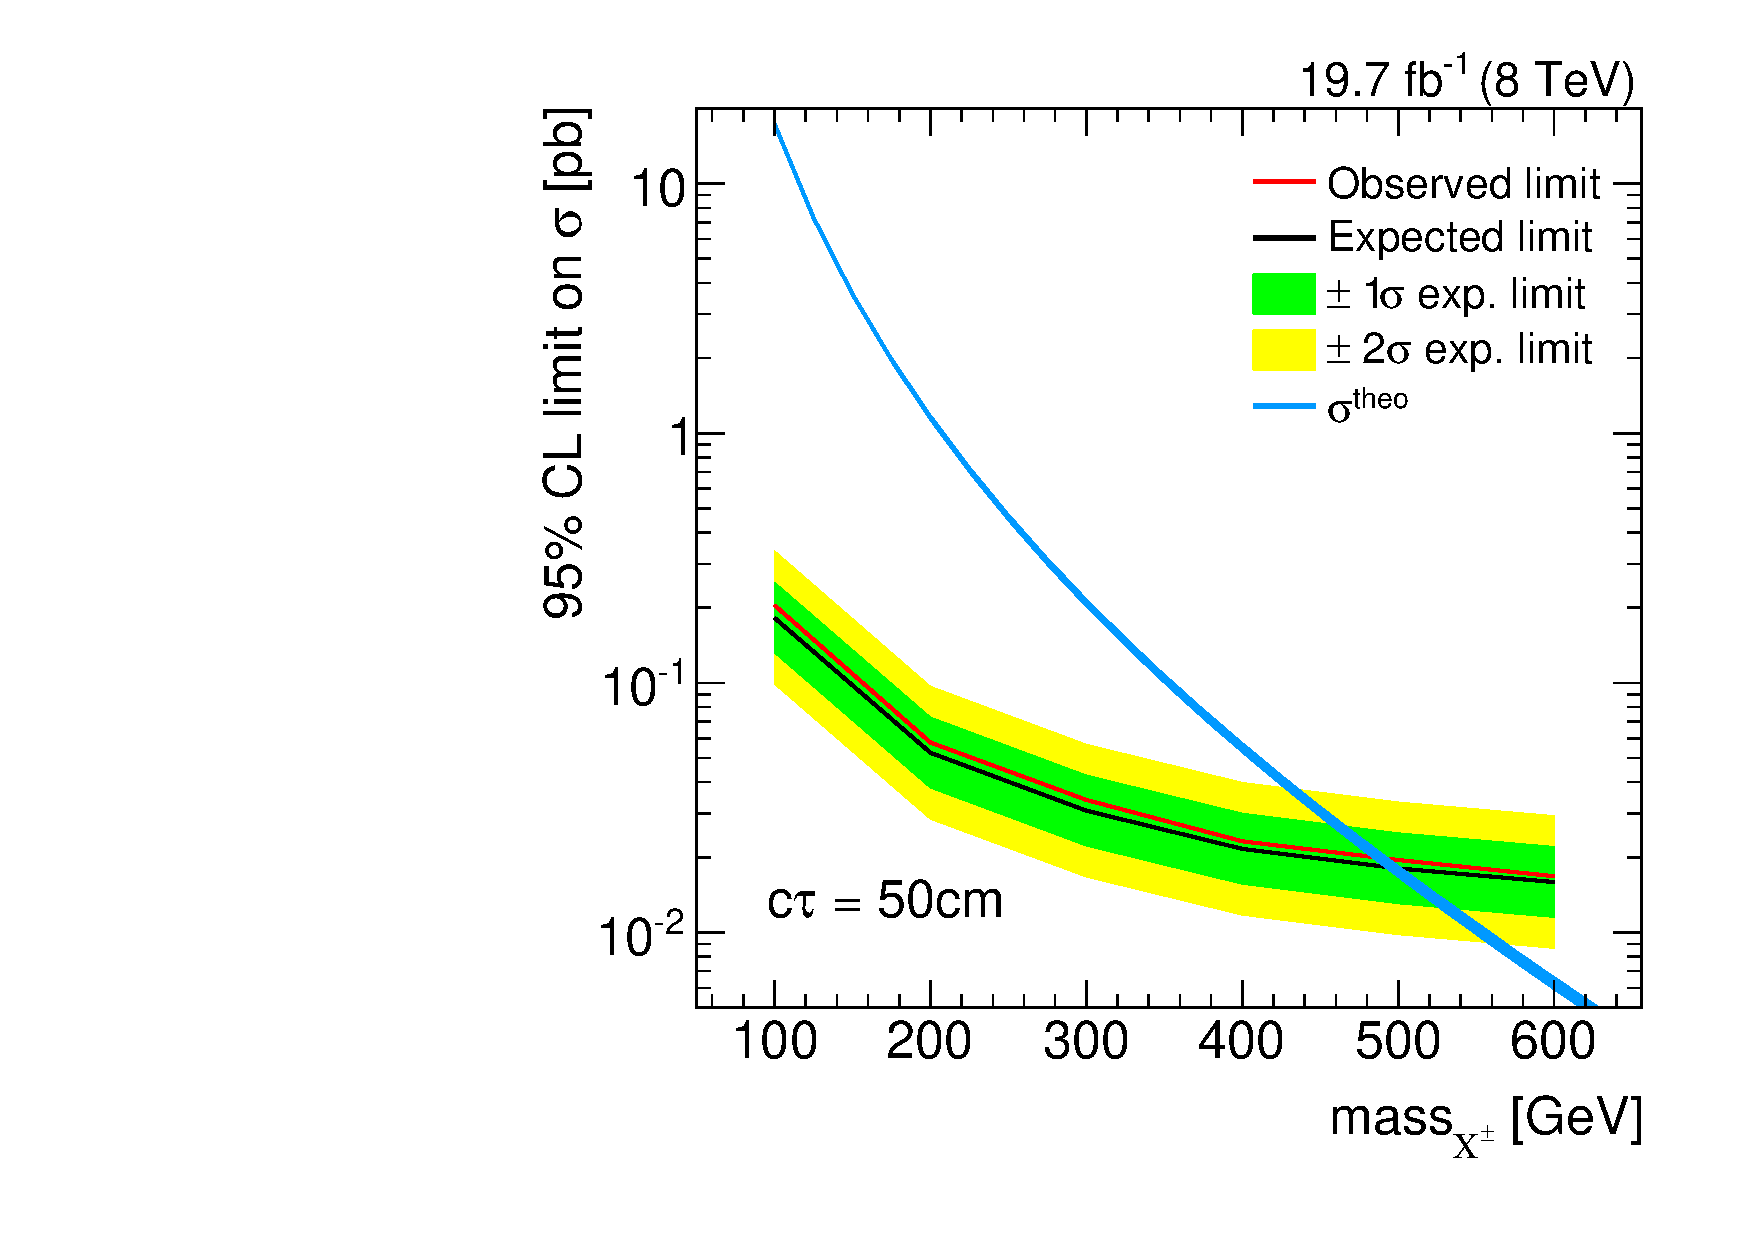
\includegraphics[width=0.29\textwidth]{figures/analysis/Interpretation/ExclusionLimits/LimitPlot_ctau50cm.pdf} 
    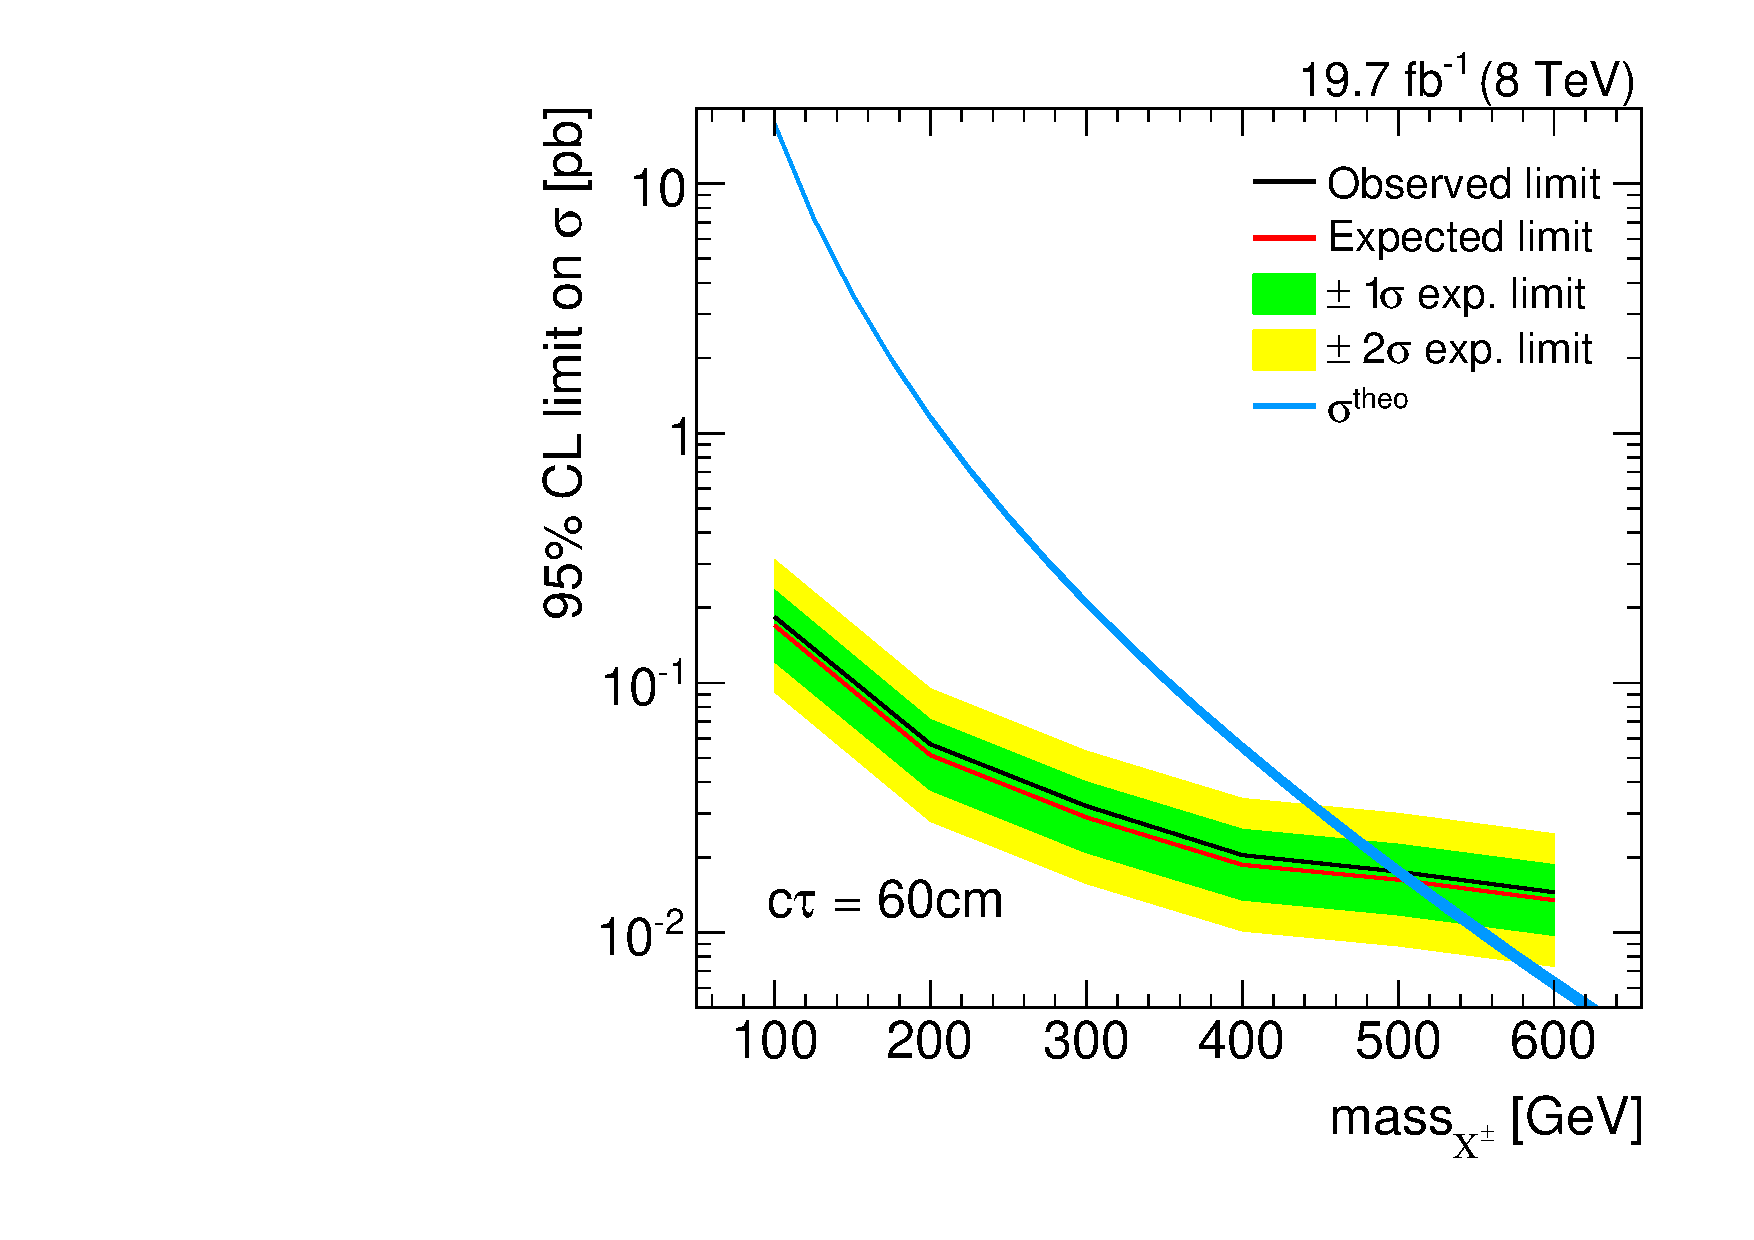
\includegraphics[width=0.29\textwidth]{figures/analysis/Interpretation/ExclusionLimits/LimitPlot_ctau60cm.pdf} \\
    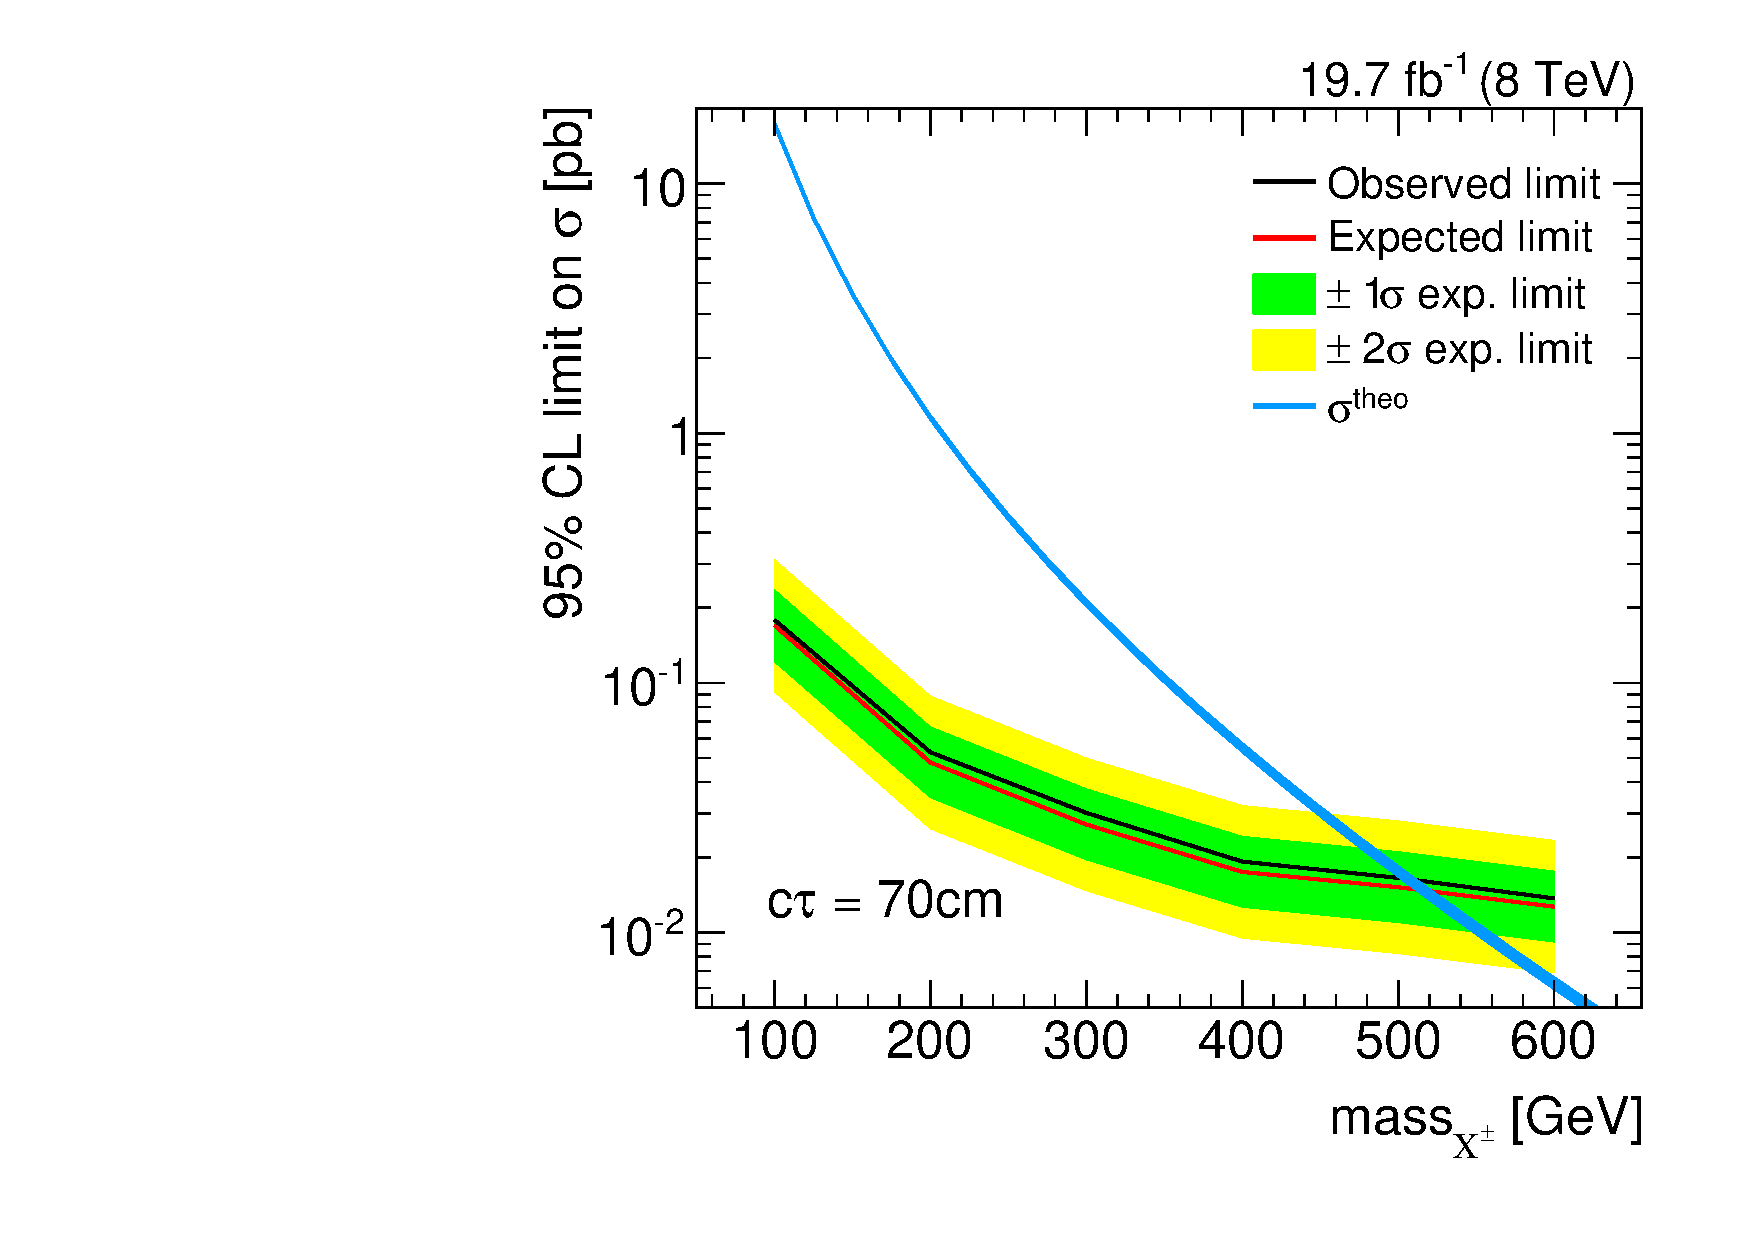
\includegraphics[width=0.29\textwidth]{figures/analysis/Interpretation/ExclusionLimits/LimitPlot_ctau70cm.pdf} 
    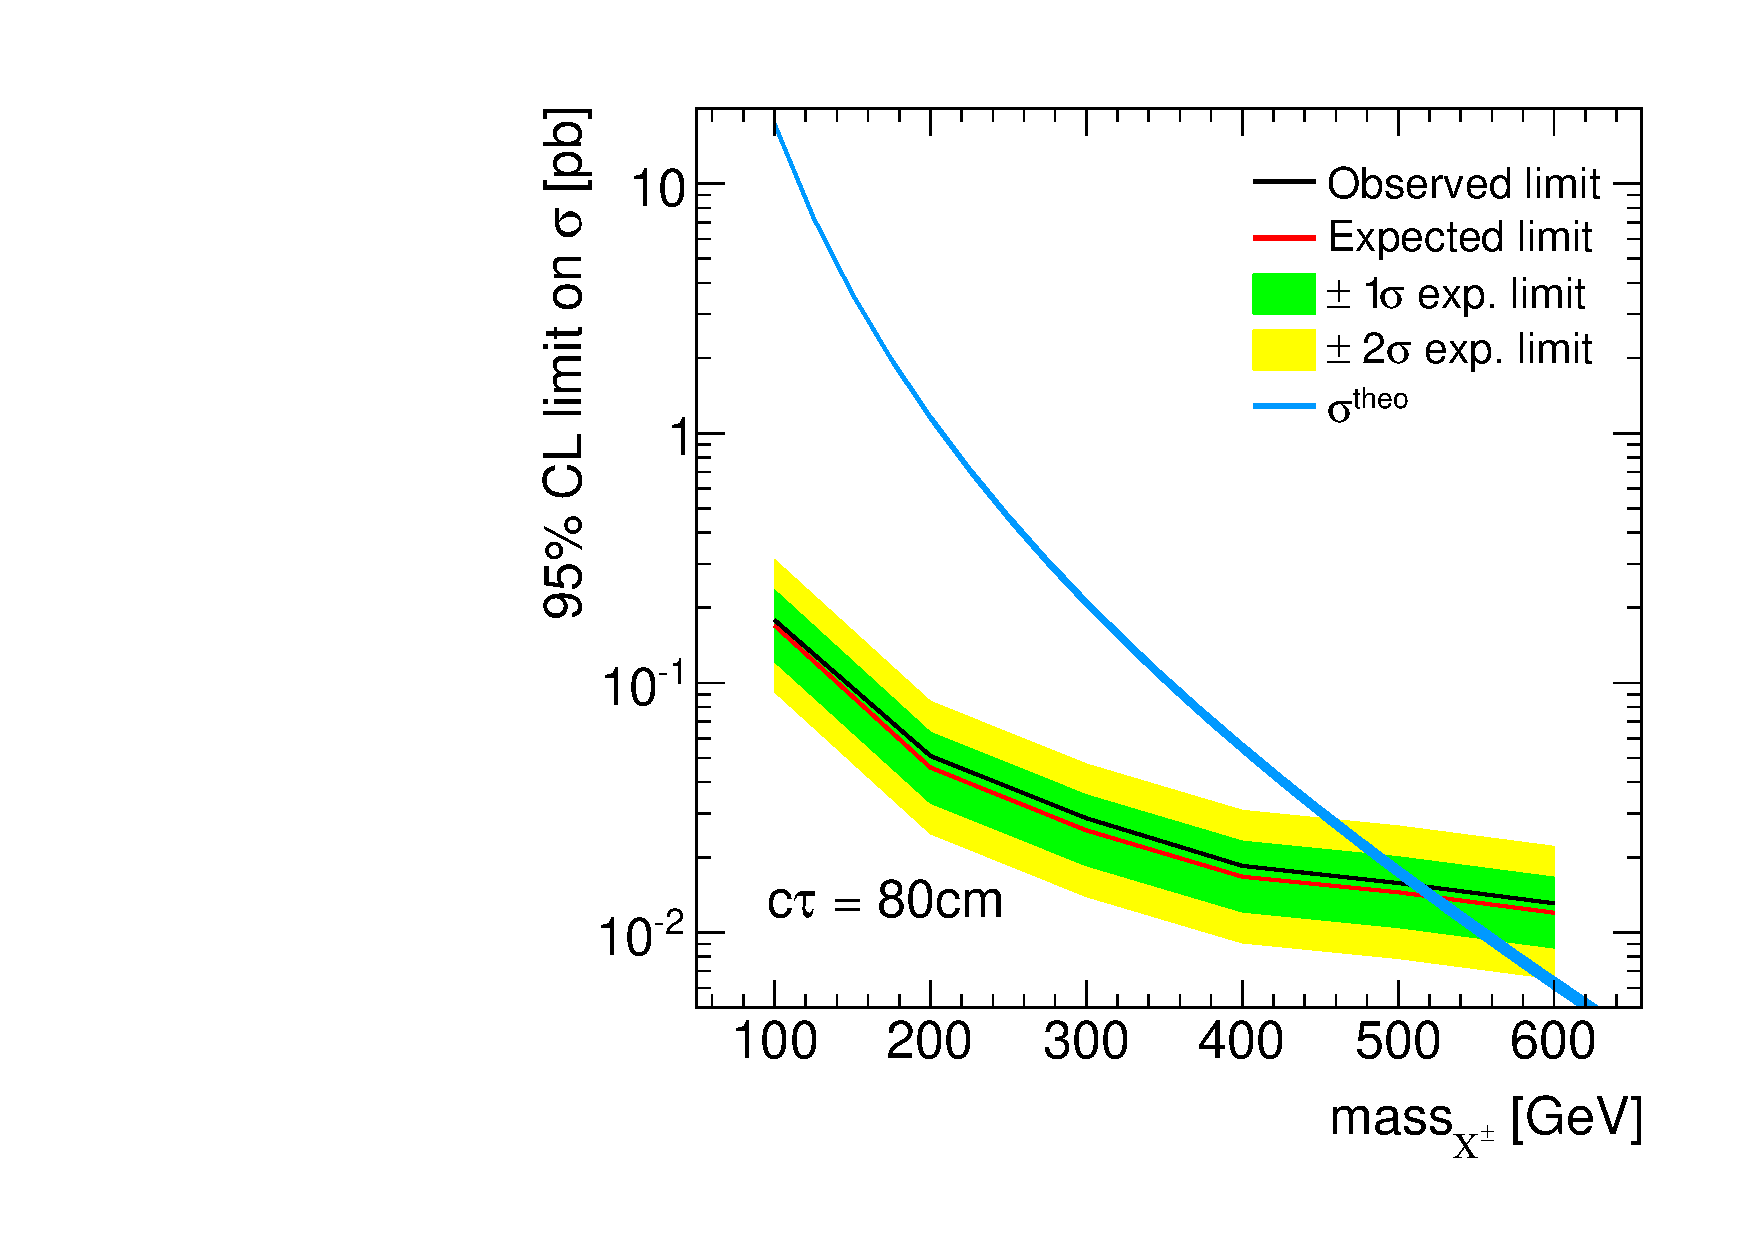
\includegraphics[width=0.29\textwidth]{figures/analysis/Interpretation/ExclusionLimits/LimitPlot_ctau80cm.pdf} 
    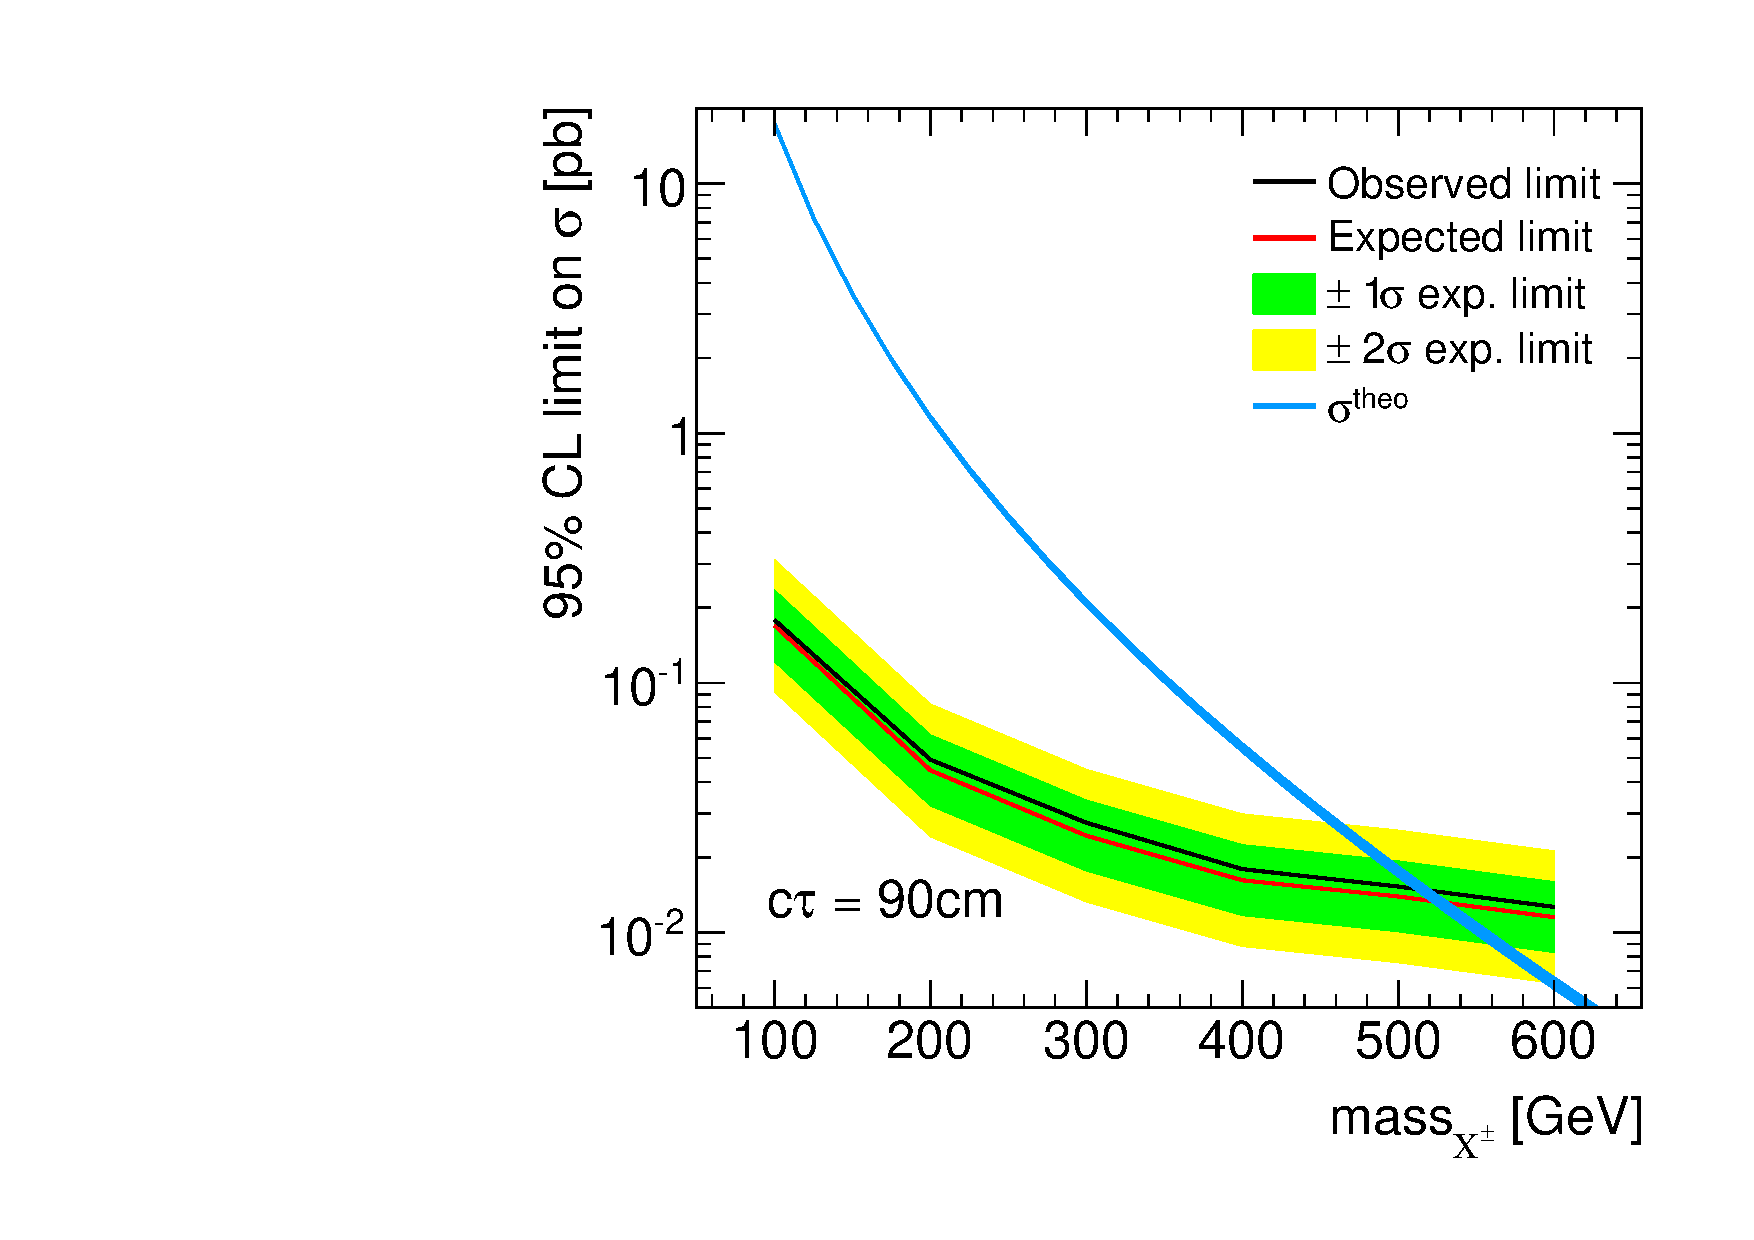
\includegraphics[width=0.29\textwidth]{figures/analysis/Interpretation/ExclusionLimits/LimitPlot_ctau90cm.pdf} \\
    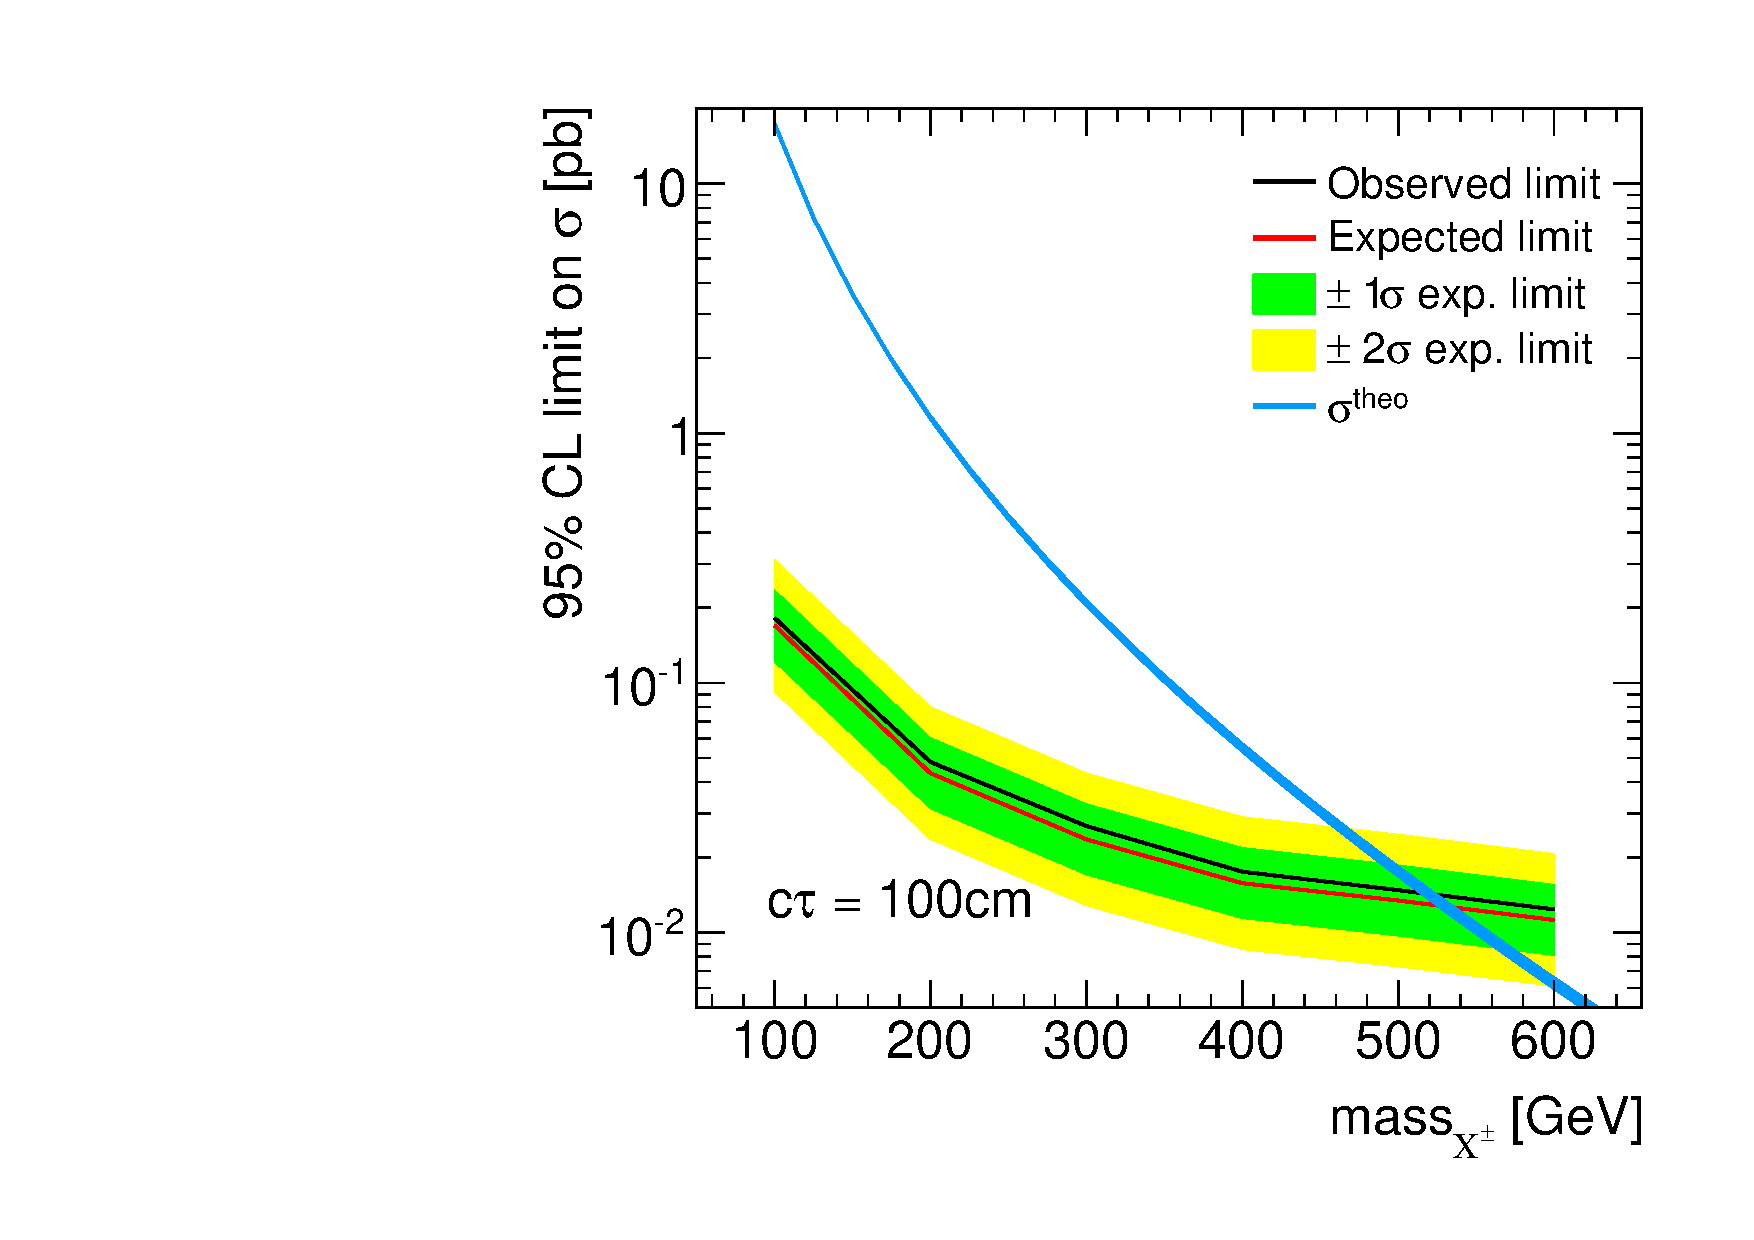
\includegraphics[width=0.29\textwidth]{figures/analysis/Interpretation/ExclusionLimits/LimitPlot_ctau100cm.pdf} 
    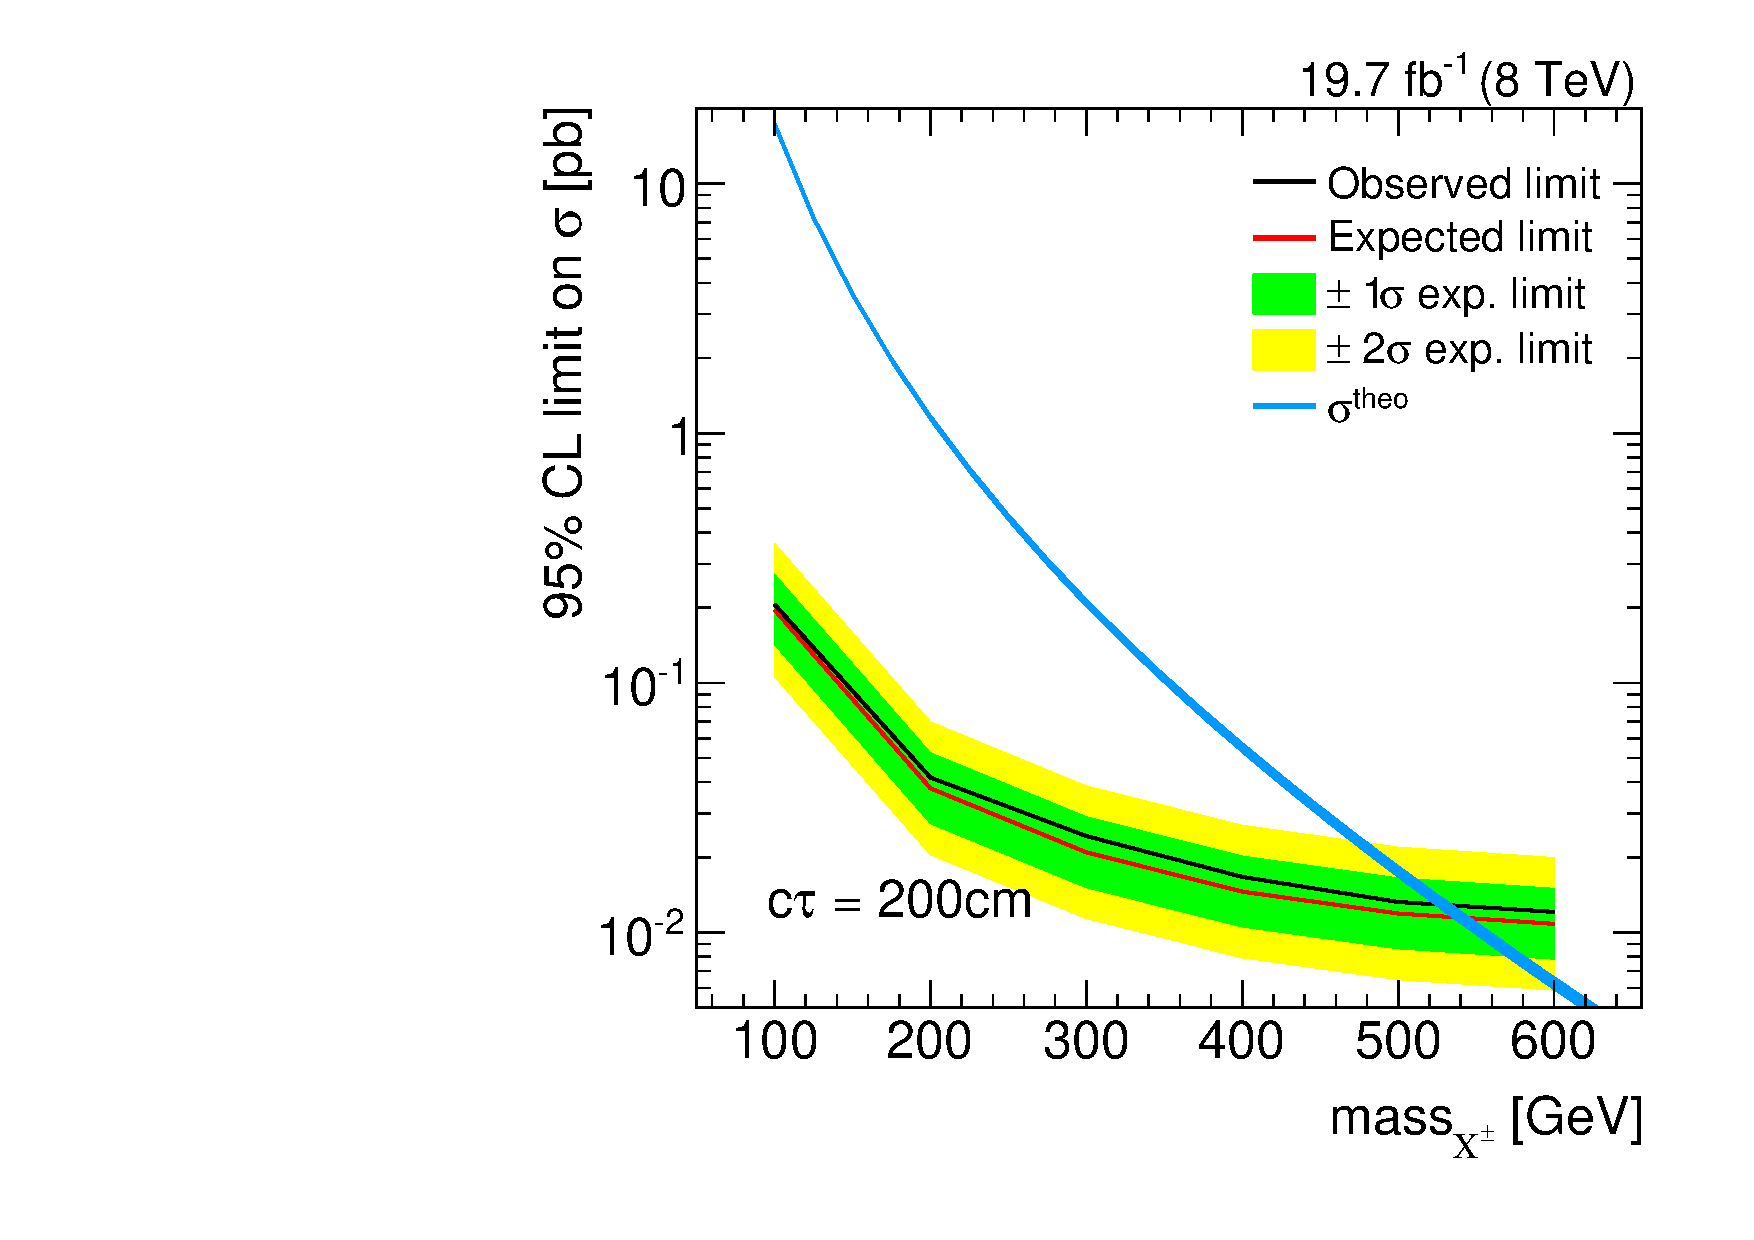
\includegraphics[width=0.29\textwidth]{figures/analysis/Interpretation/ExclusionLimits/LimitPlot_ctau200cm.pdf} 
    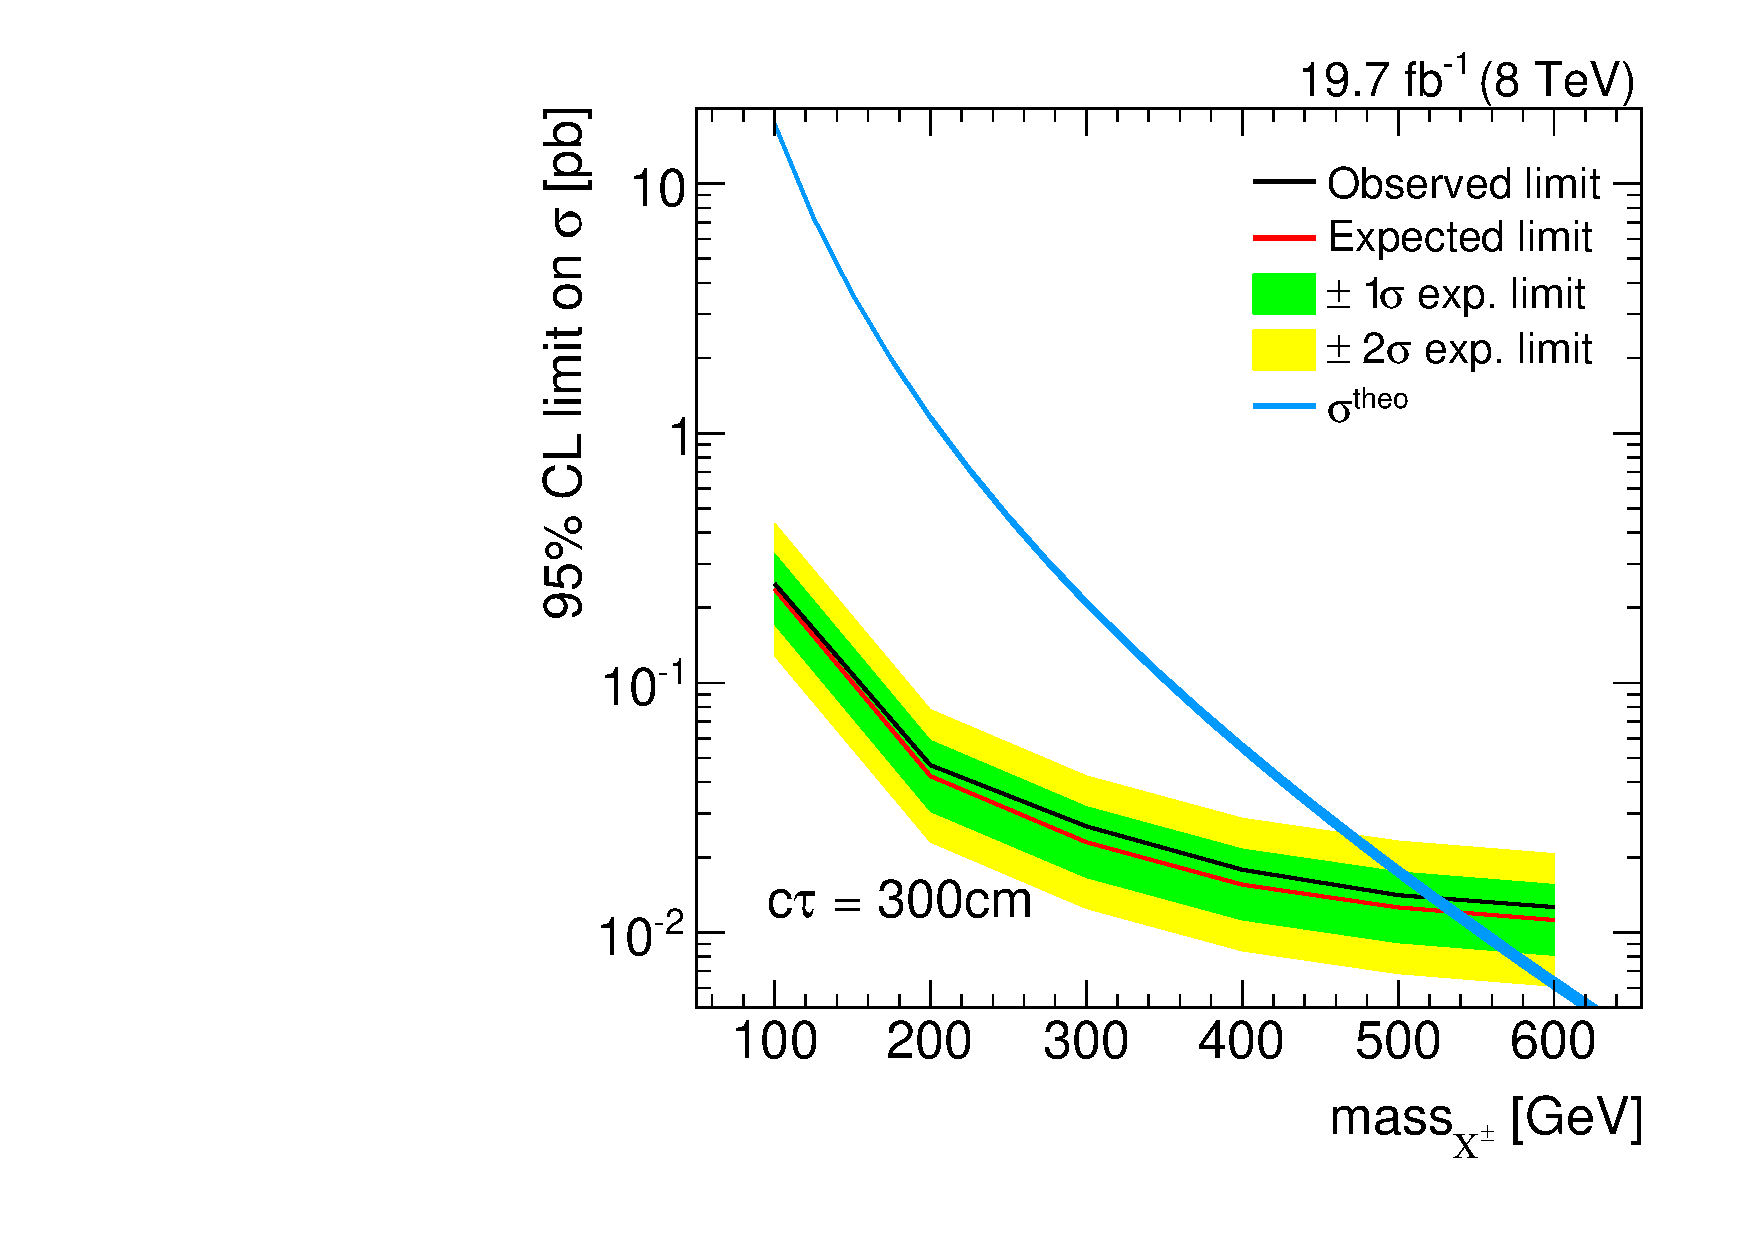
\includegraphics[width=0.29\textwidth]{figures/analysis/Interpretation/ExclusionLimits/LimitPlot_ctau300cm.pdf} \\
    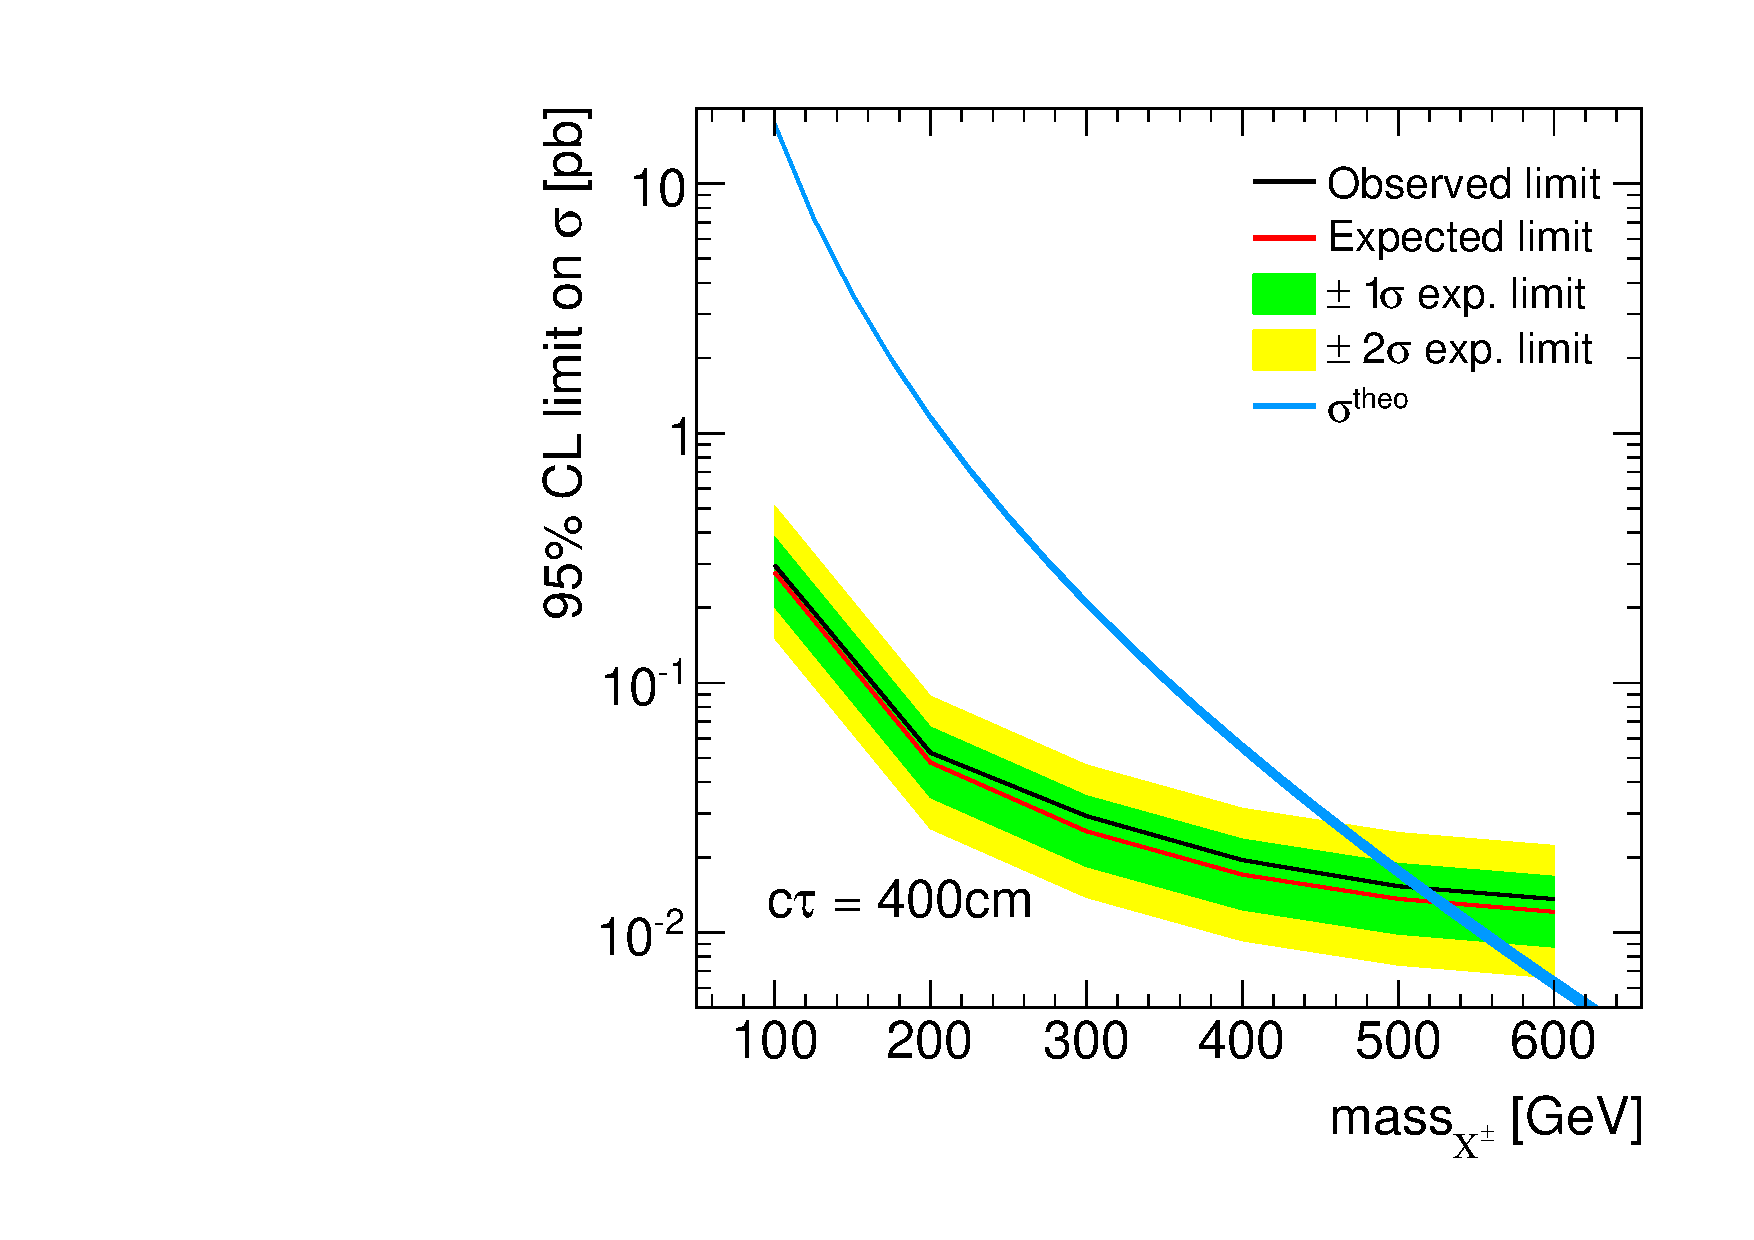
\includegraphics[width=0.29\textwidth]{figures/analysis/Interpretation/ExclusionLimits/LimitPlot_ctau400cm.pdf} 
    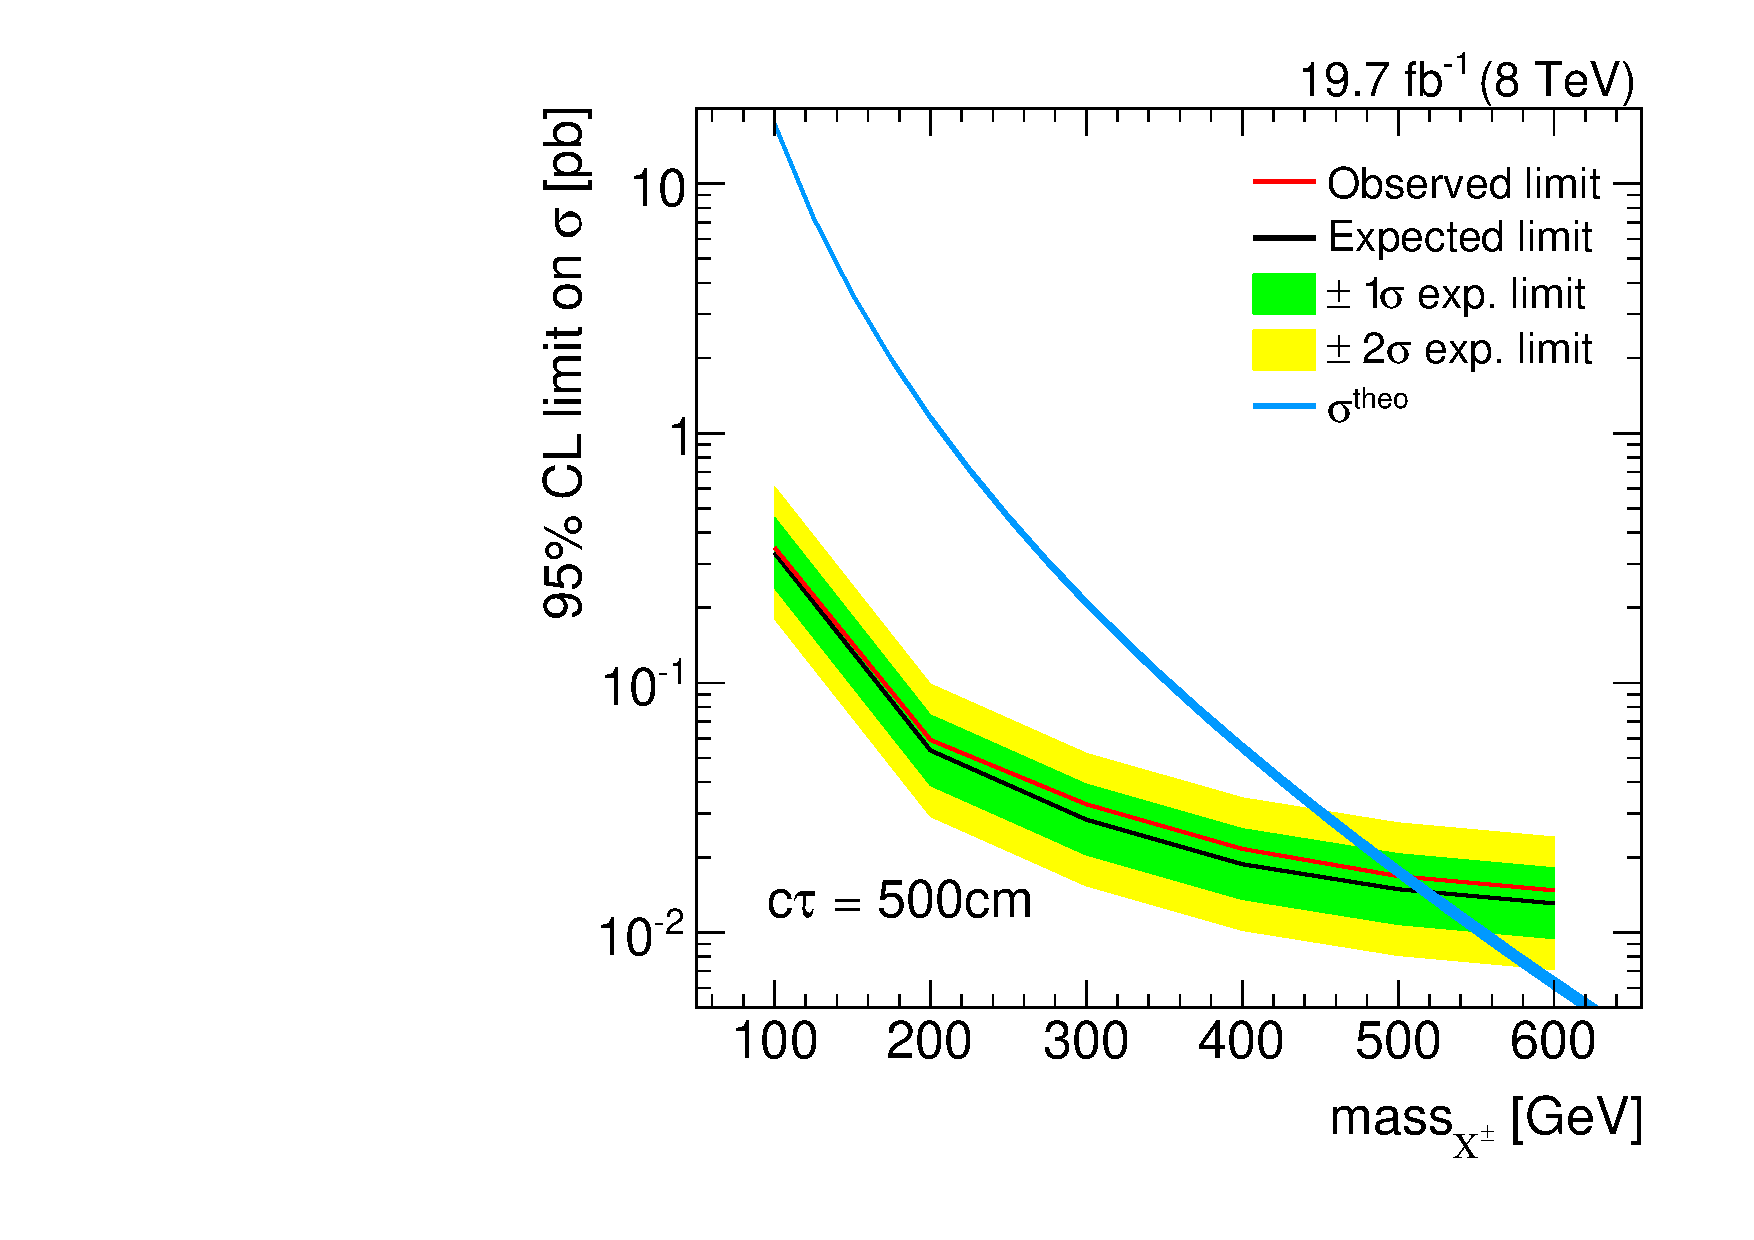
\includegraphics[width=0.29\textwidth]{figures/analysis/Interpretation/ExclusionLimits/LimitPlot_ctau500cm.pdf} 
    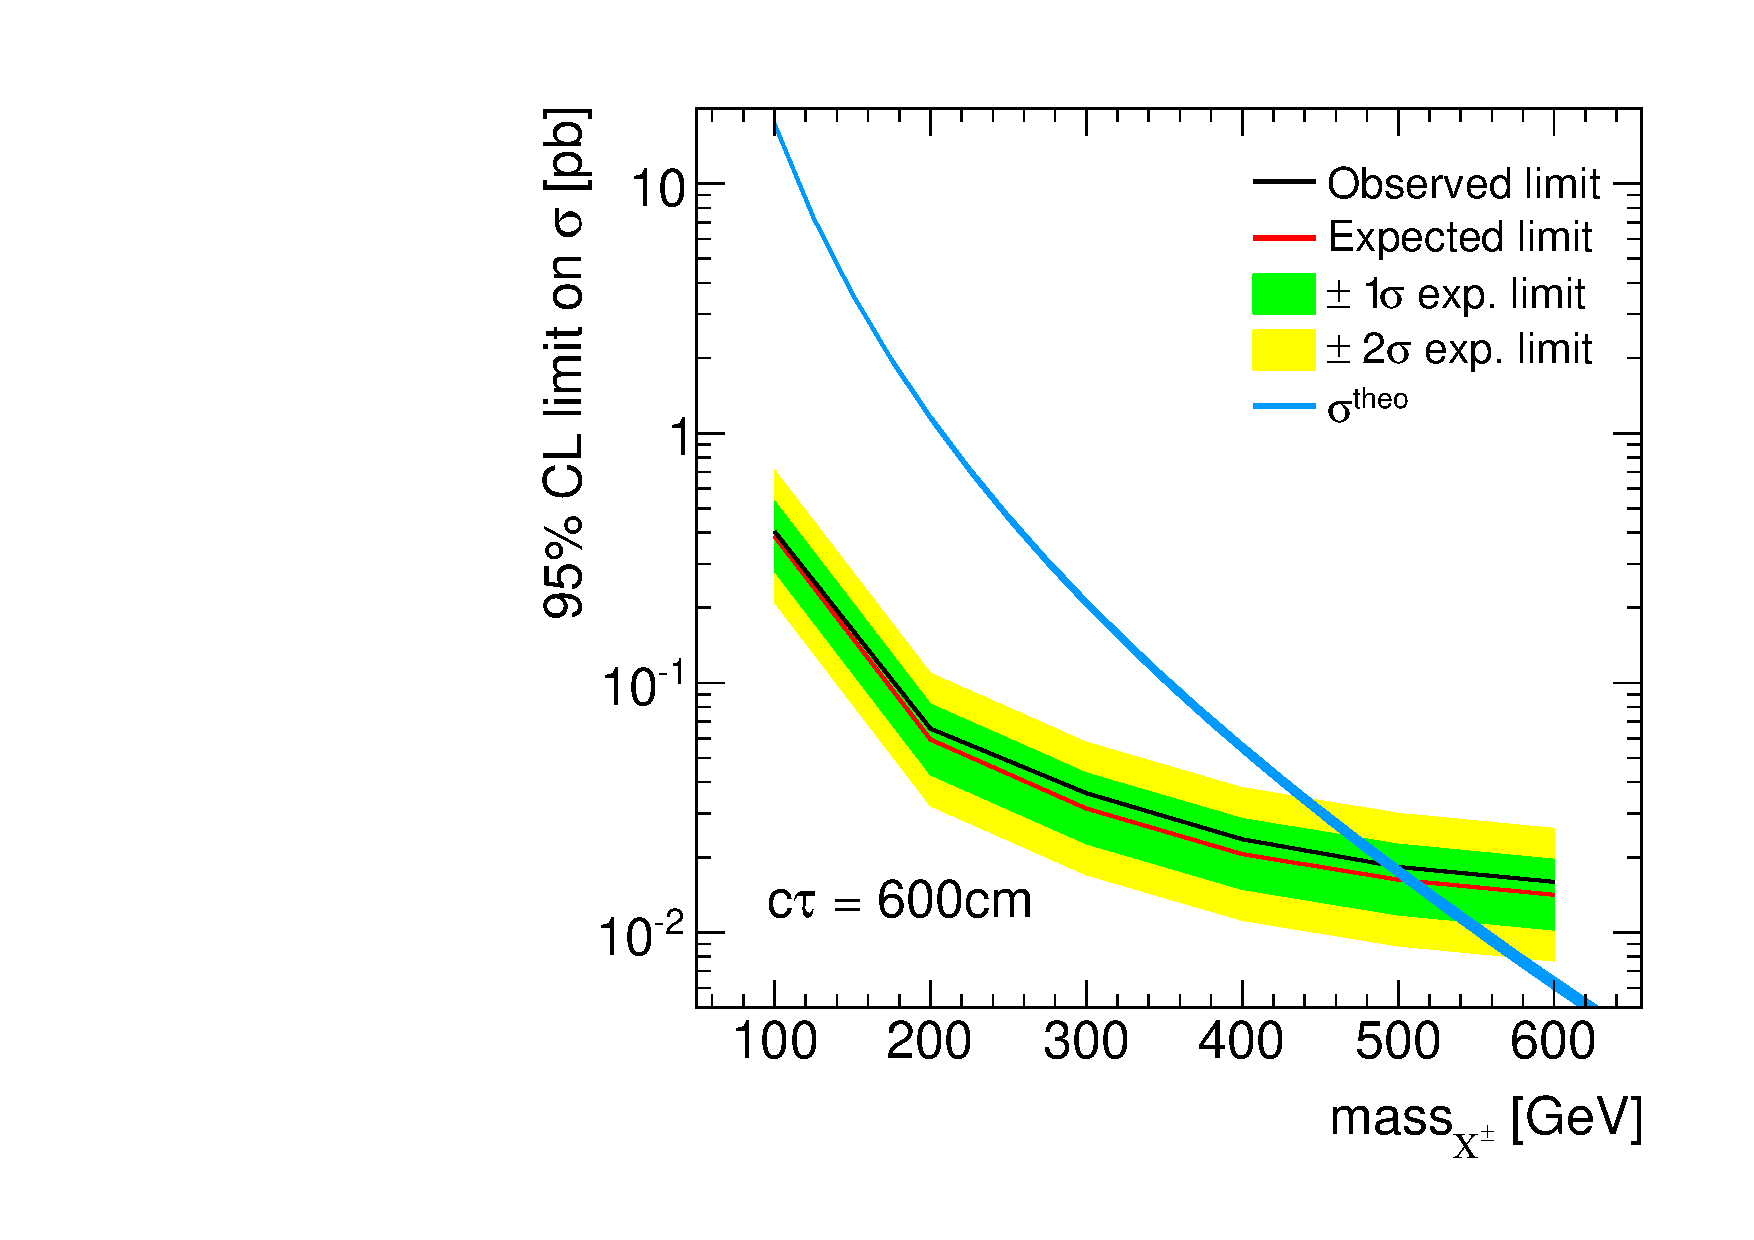
\includegraphics[width=0.29\textwidth]{figures/analysis/Interpretation/ExclusionLimits/LimitPlot_ctau600cm.pdf} \\
  \end{tabular}
  \caption{95\% CL exclusion limits for signal models with $\ctau = 40-600\cm$.}
  \label{fig:1dLimitsB}
\end{figure} 

\begin{figure}[!h]
  \centering 
  \begin{tabular}{c}
    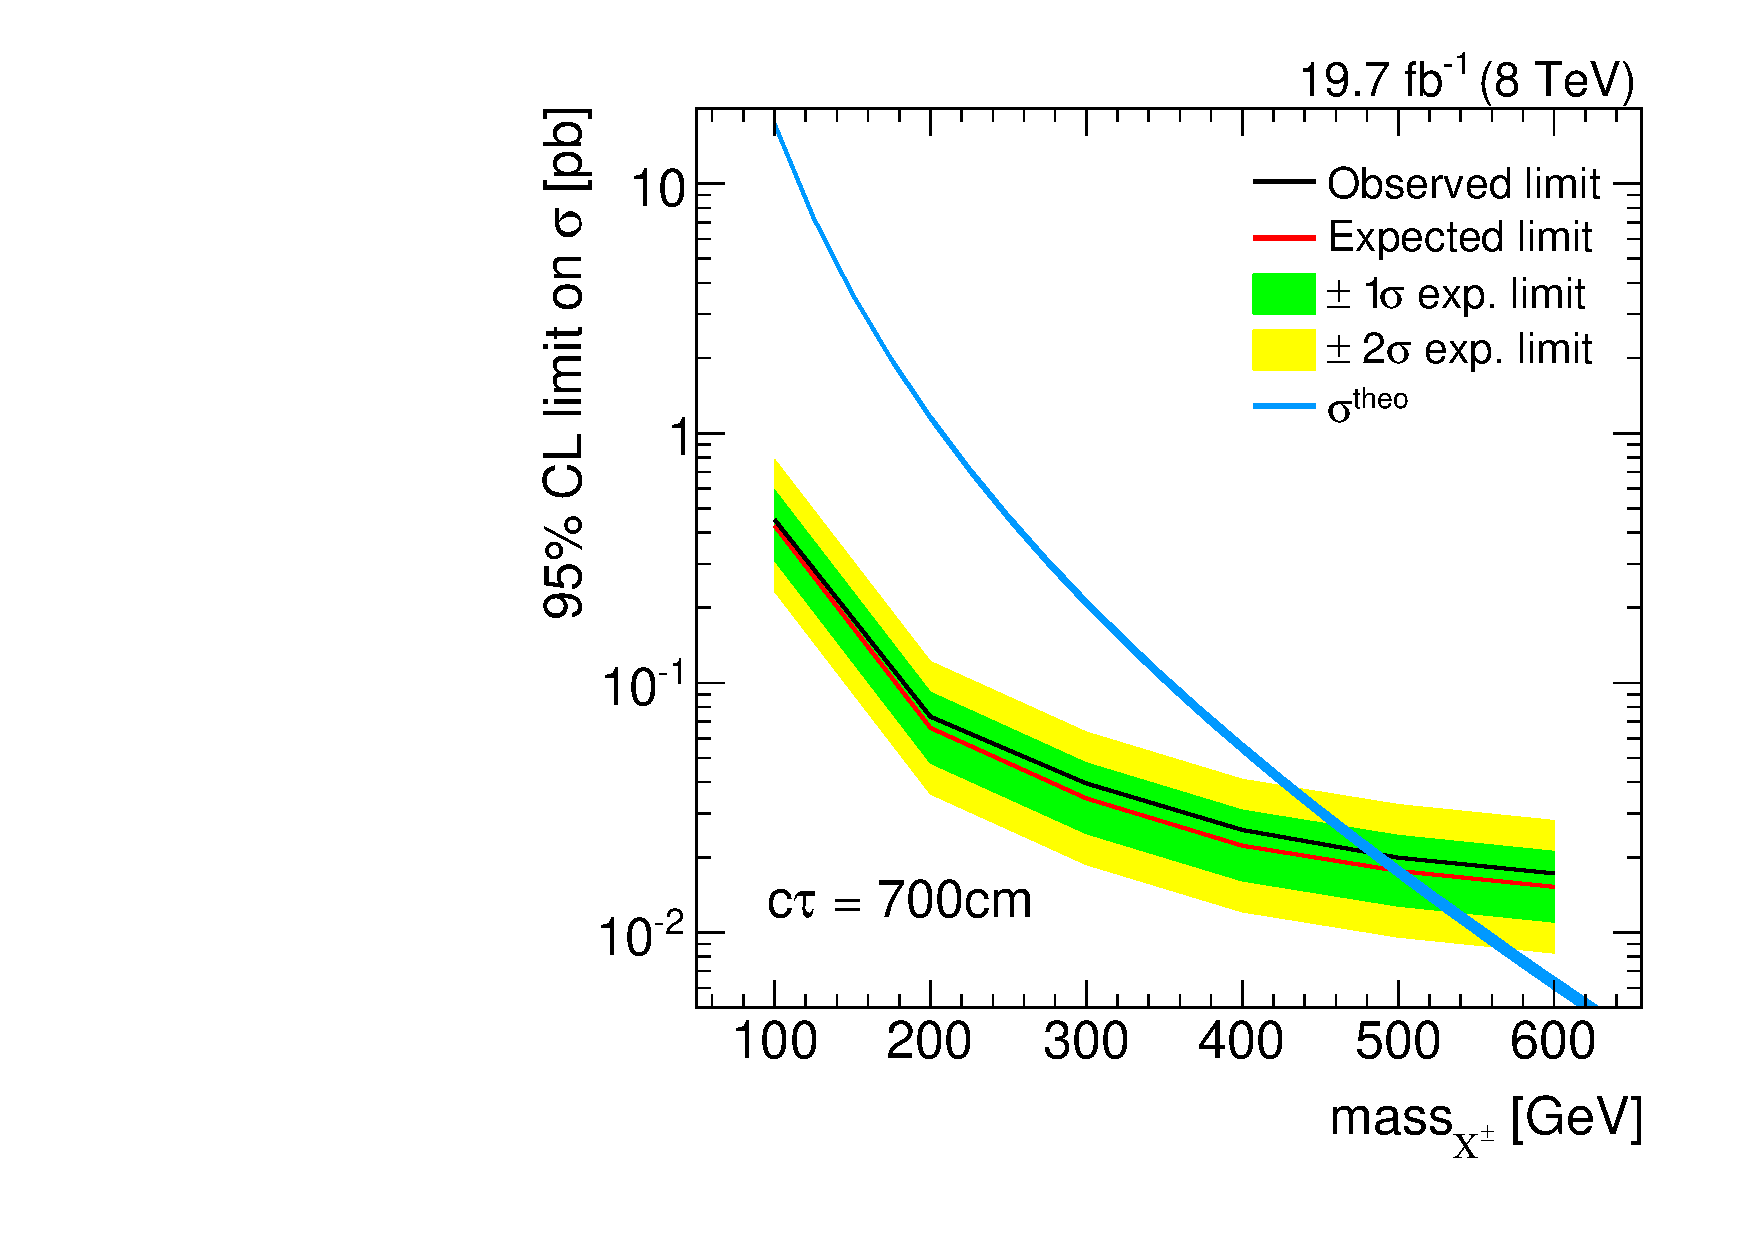
\includegraphics[width=0.29\textwidth]{figures/analysis/Interpretation/ExclusionLimits/LimitPlot_ctau700cm.pdf} 
    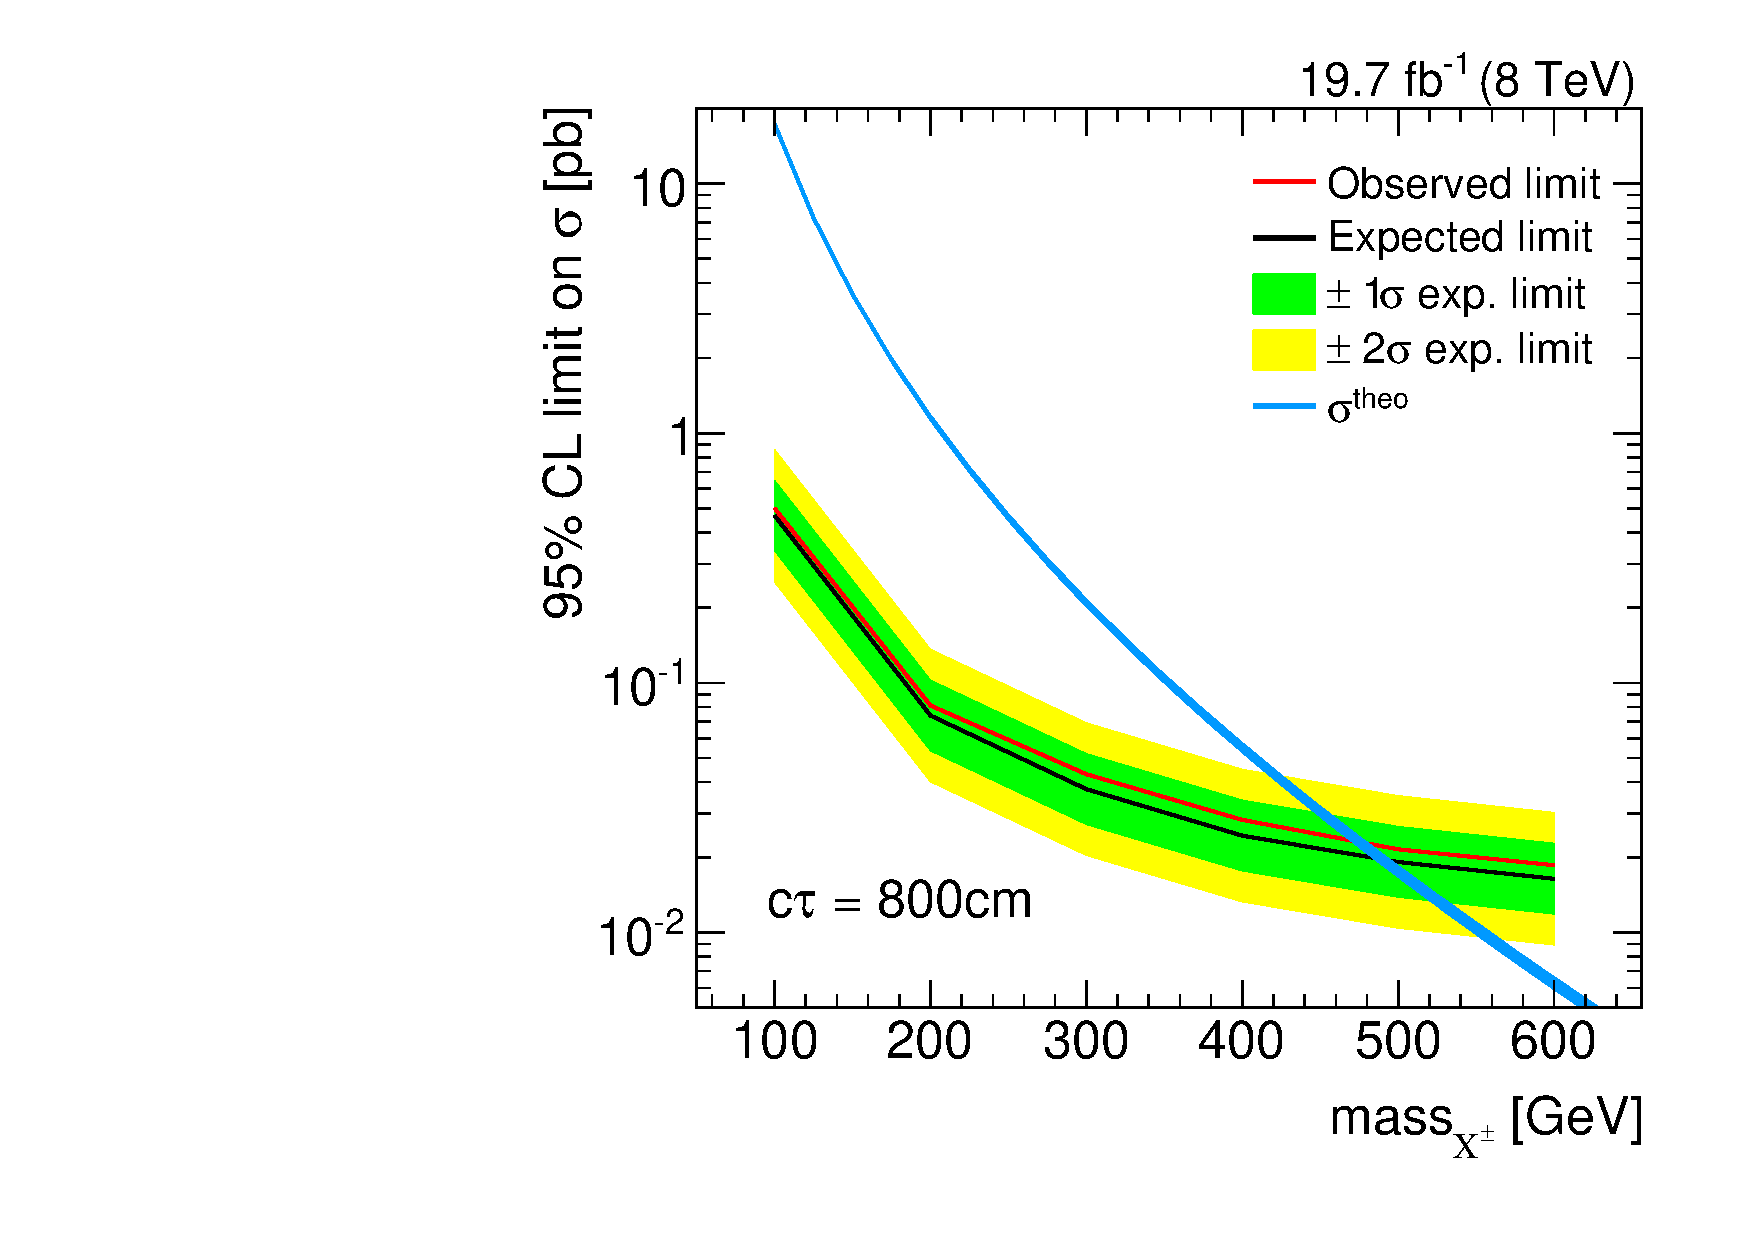
\includegraphics[width=0.29\textwidth]{figures/analysis/Interpretation/ExclusionLimits/LimitPlot_ctau800cm.pdf} 
    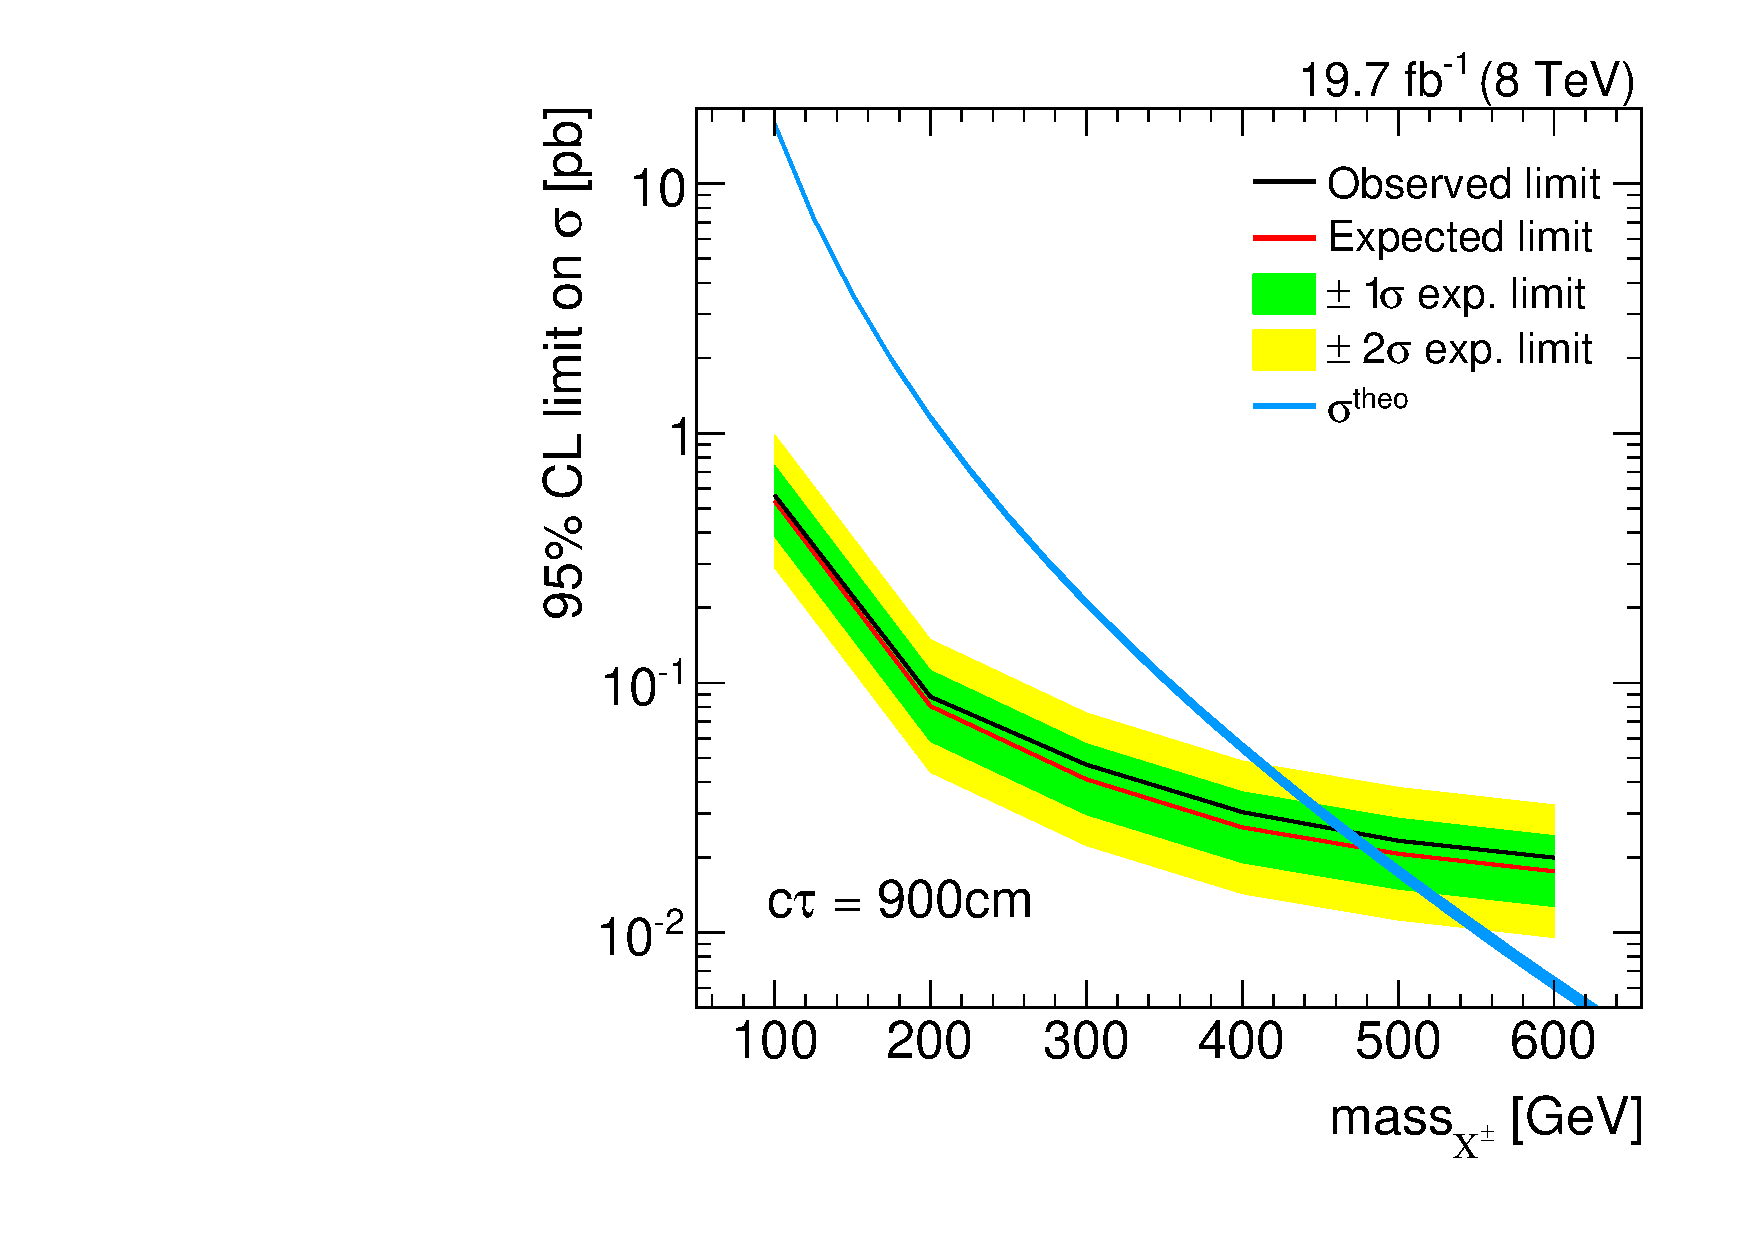
\includegraphics[width=0.29\textwidth]{figures/analysis/Interpretation/ExclusionLimits/LimitPlot_ctau900cm.pdf} \\
    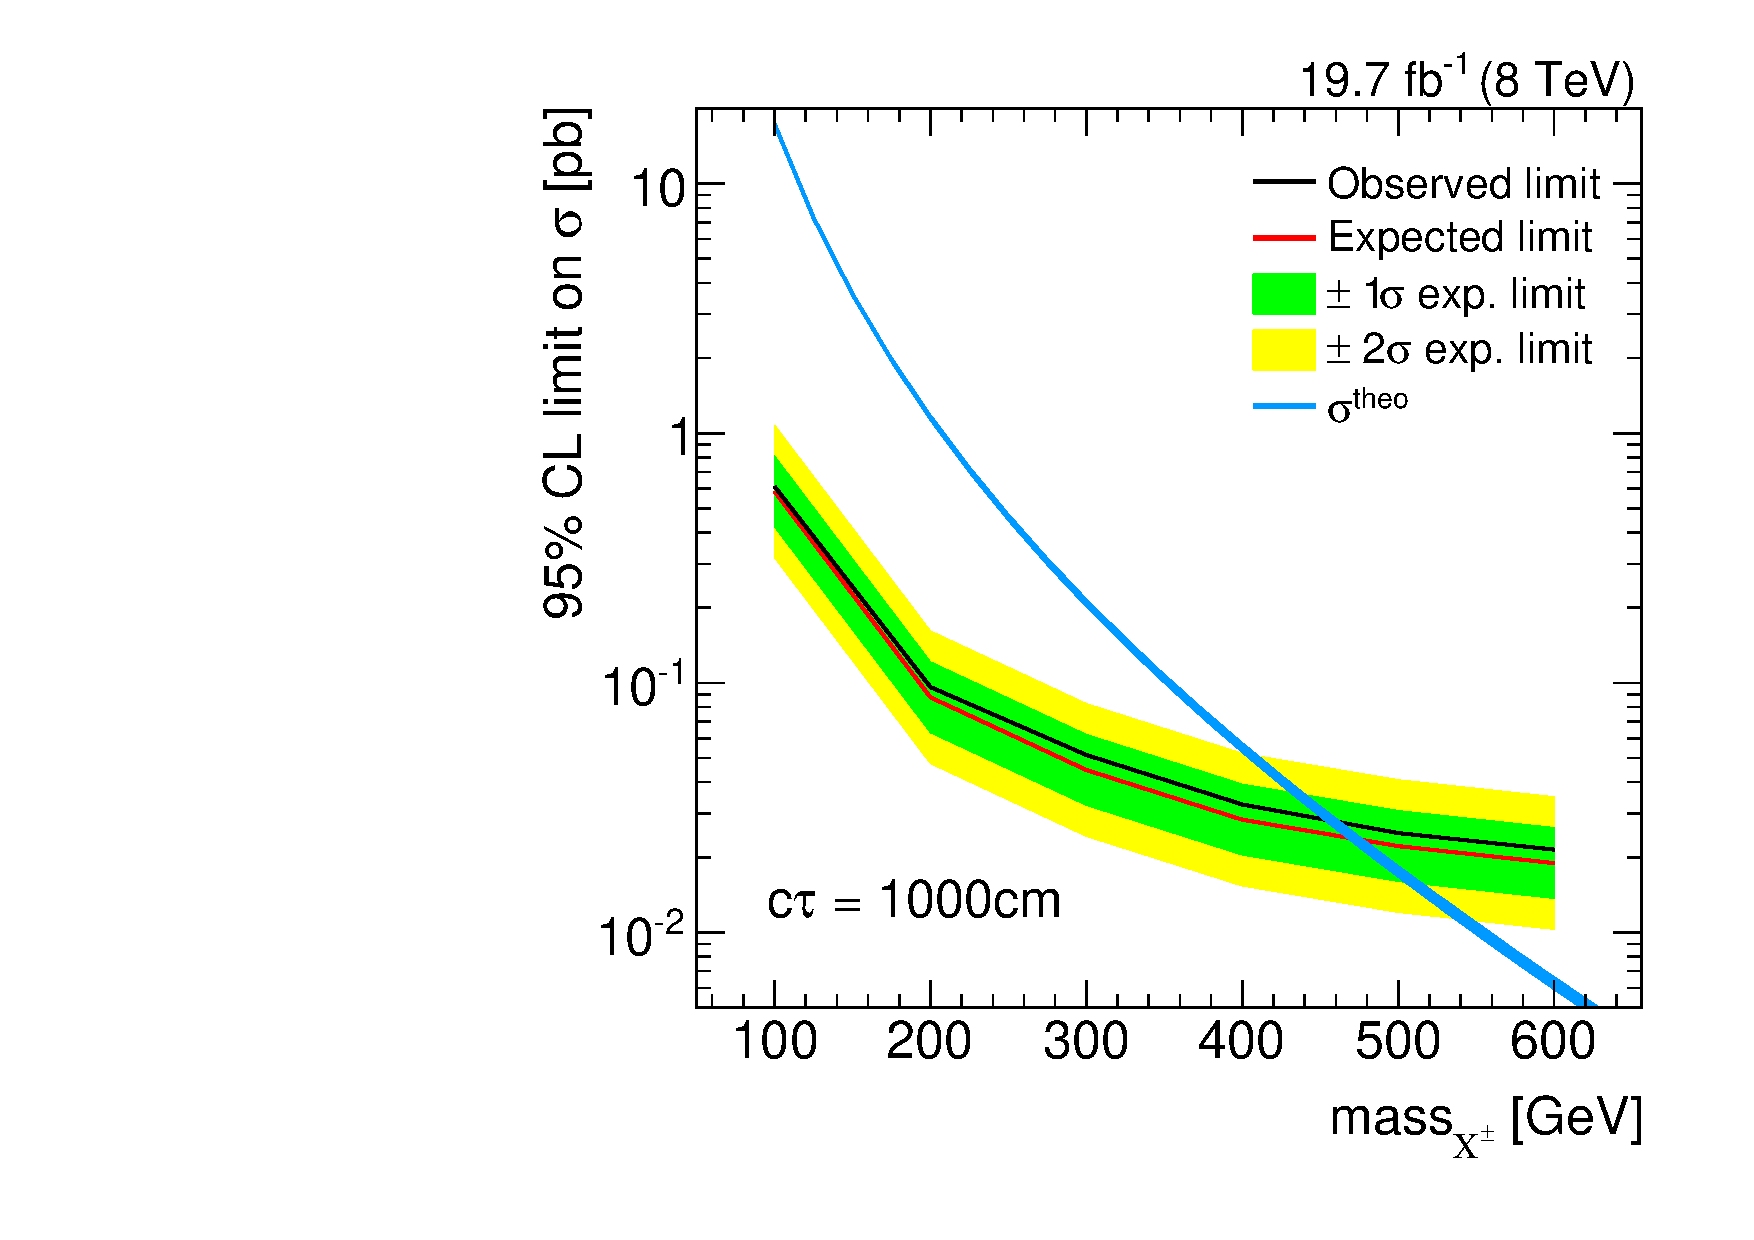
\includegraphics[width=0.29\textwidth]{figures/analysis/Interpretation/ExclusionLimits/LimitPlot_ctau1000cm.pdf} 
    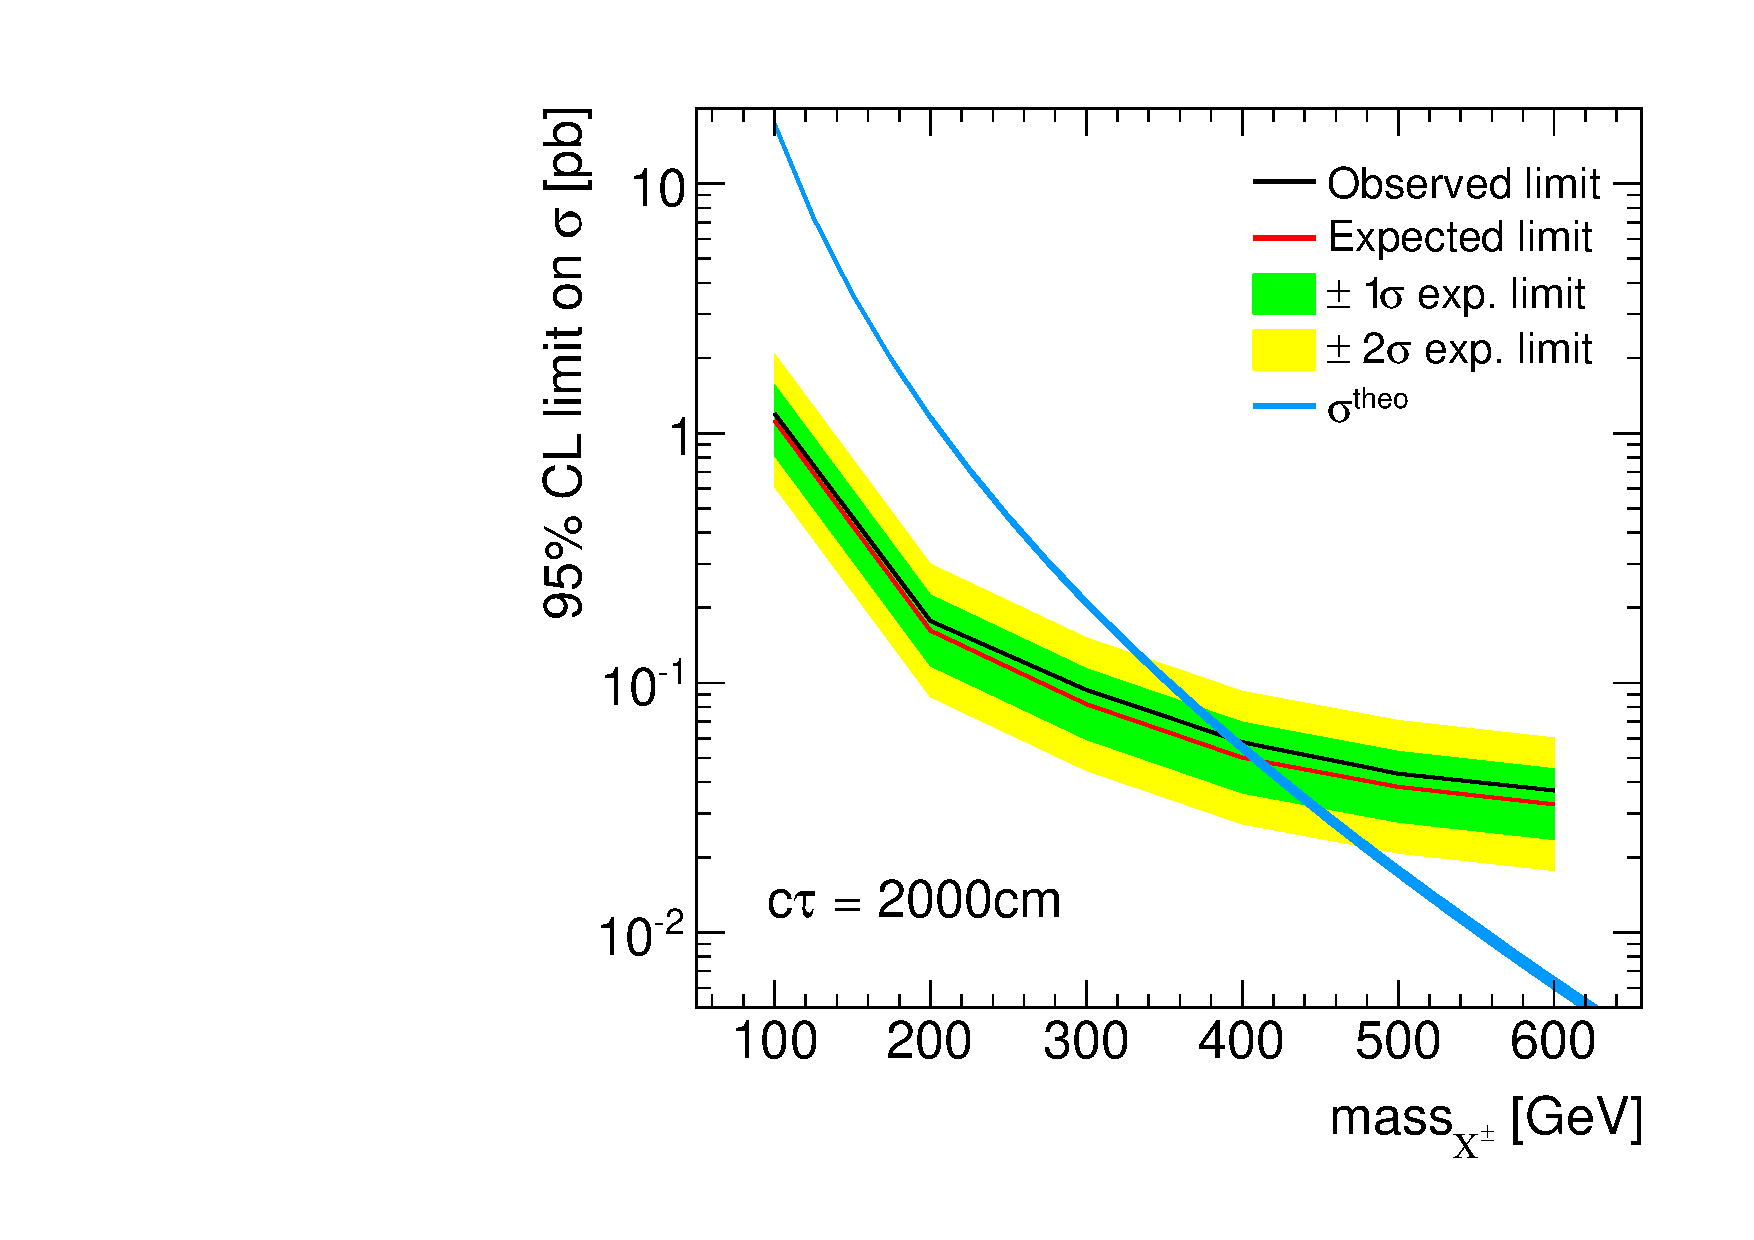
\includegraphics[width=0.29\textwidth]{figures/analysis/Interpretation/ExclusionLimits/LimitPlot_ctau2000cm.pdf} 
    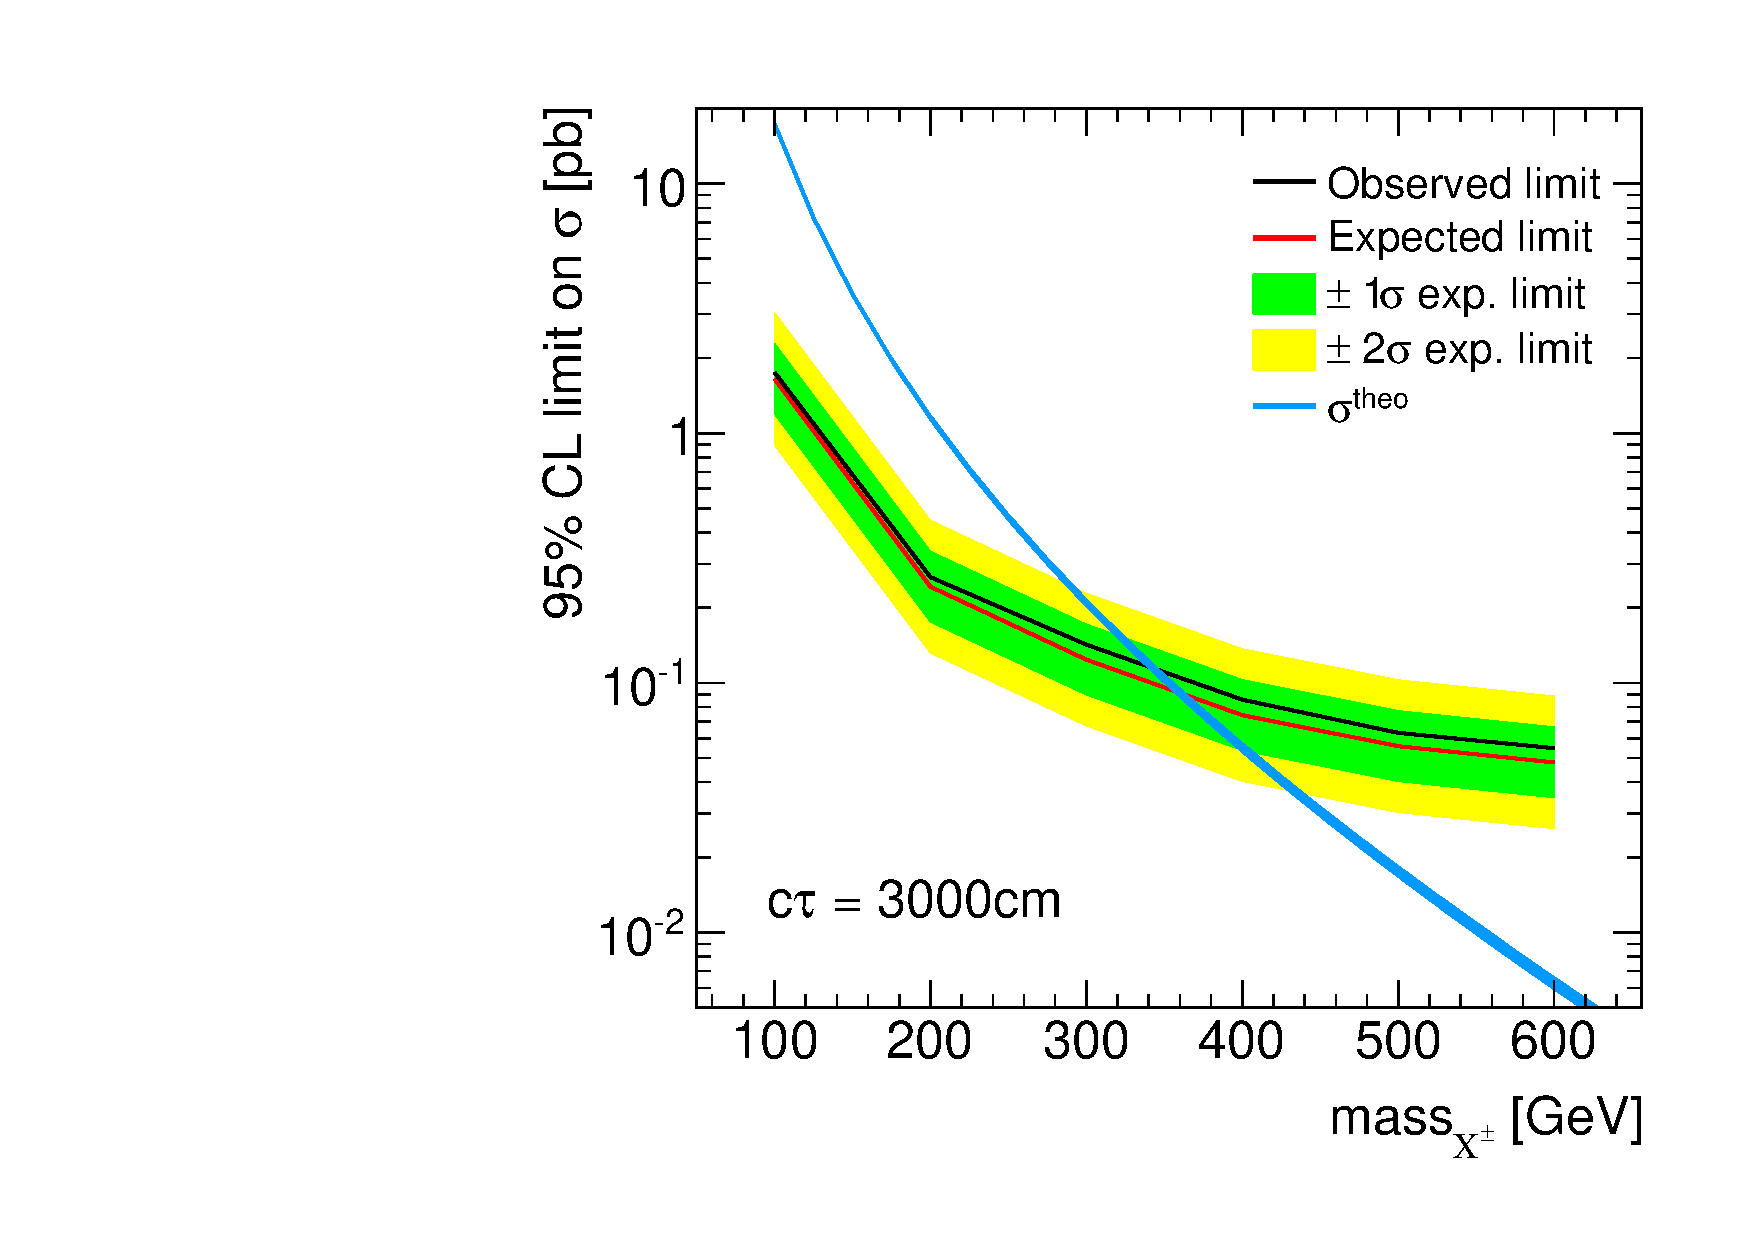
\includegraphics[width=0.29\textwidth]{figures/analysis/Interpretation/ExclusionLimits/LimitPlot_ctau3000cm.pdf} \\
    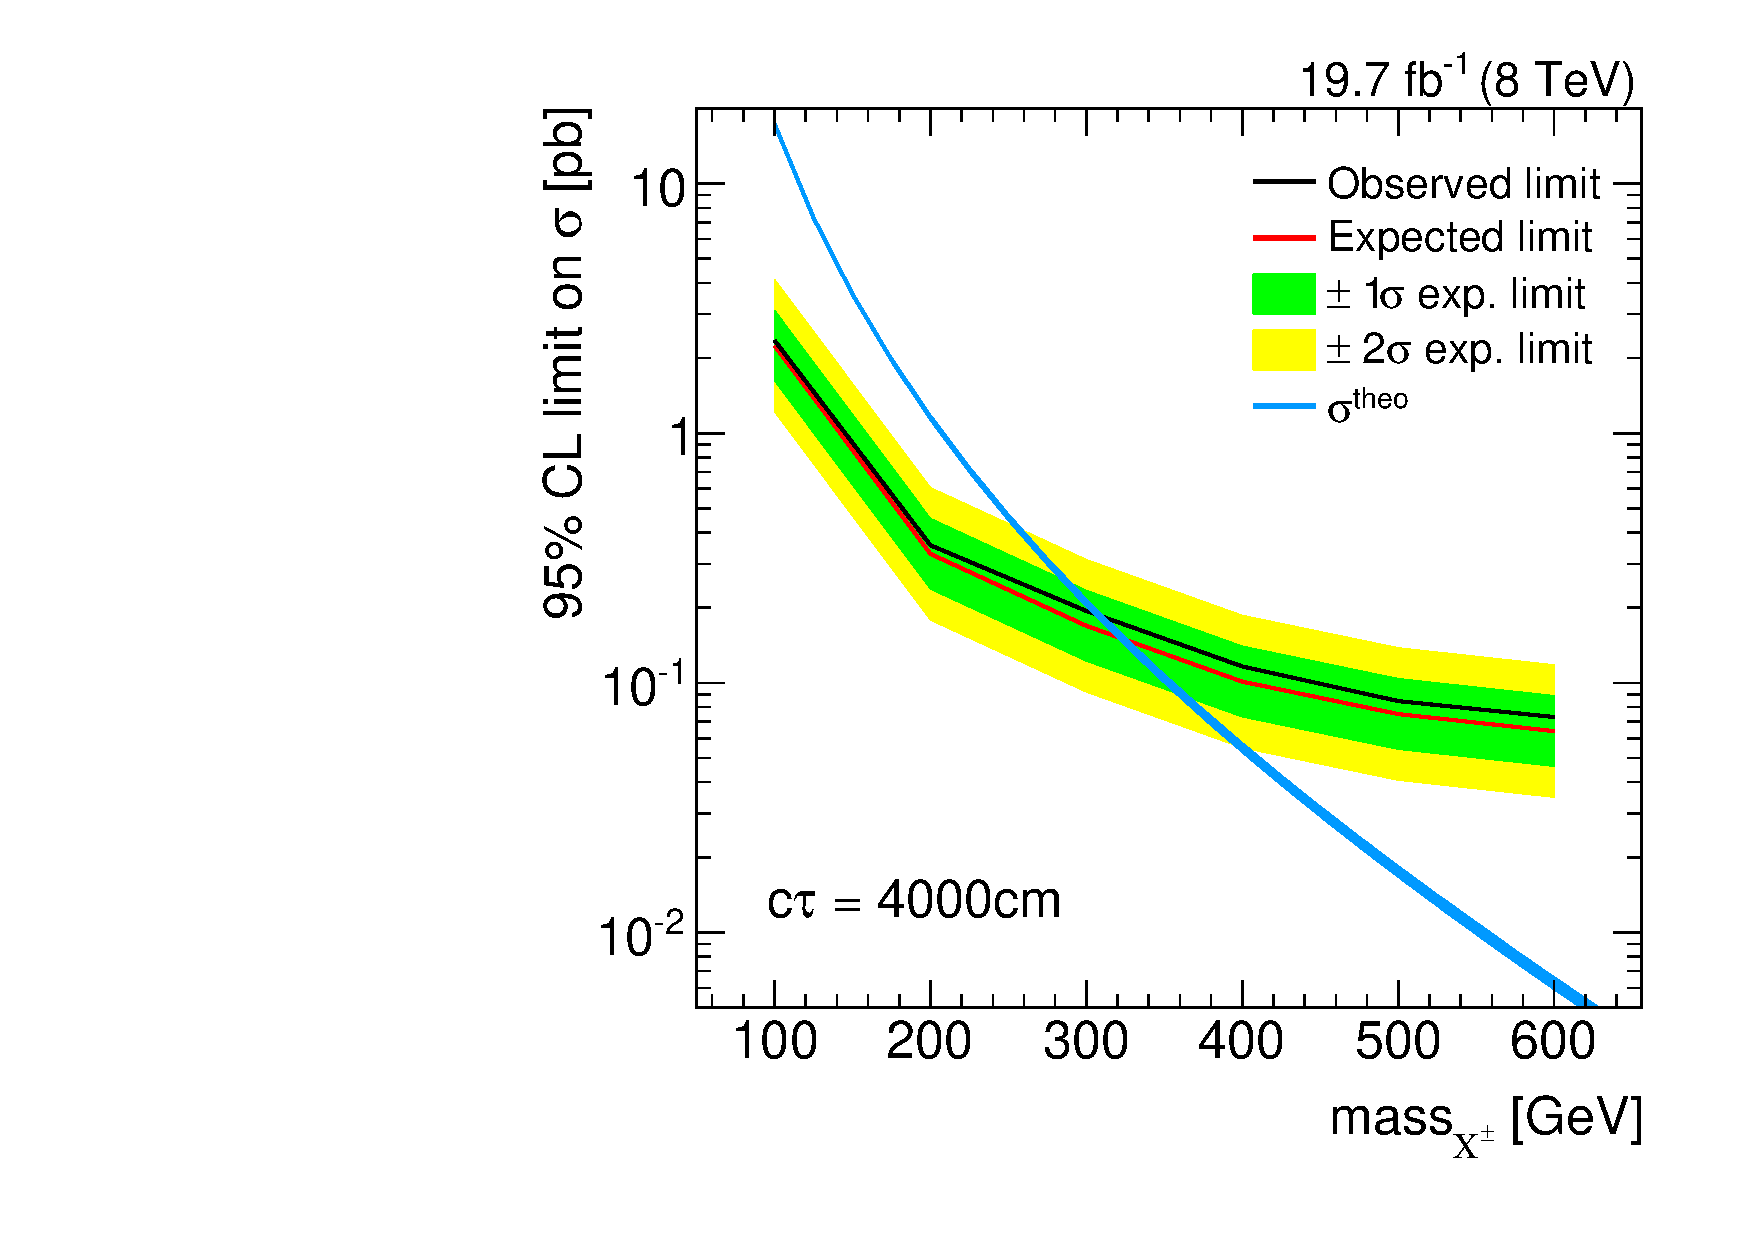
\includegraphics[width=0.29\textwidth]{figures/analysis/Interpretation/ExclusionLimits/LimitPlot_ctau4000cm.pdf} 
    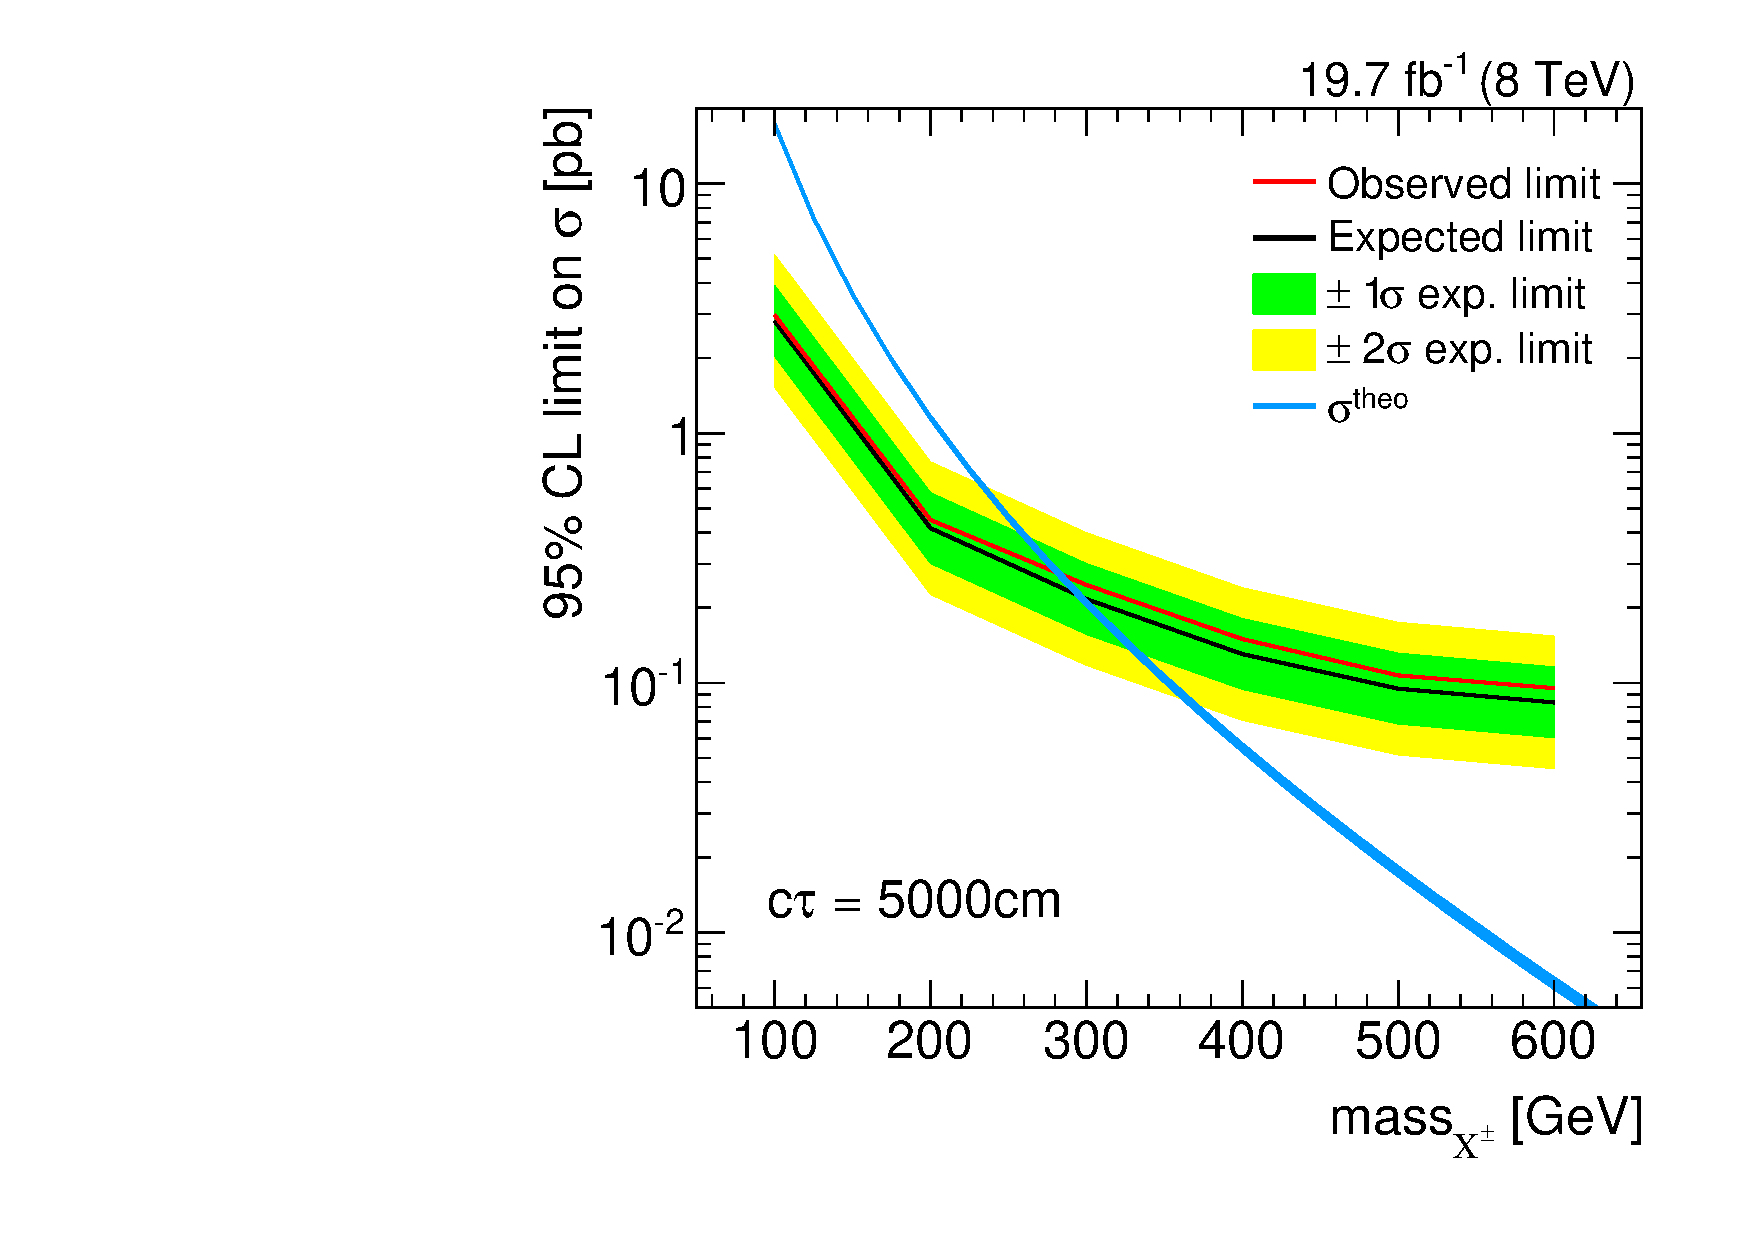
\includegraphics[width=0.29\textwidth]{figures/analysis/Interpretation/ExclusionLimits/LimitPlot_ctau5000cm.pdf} 
    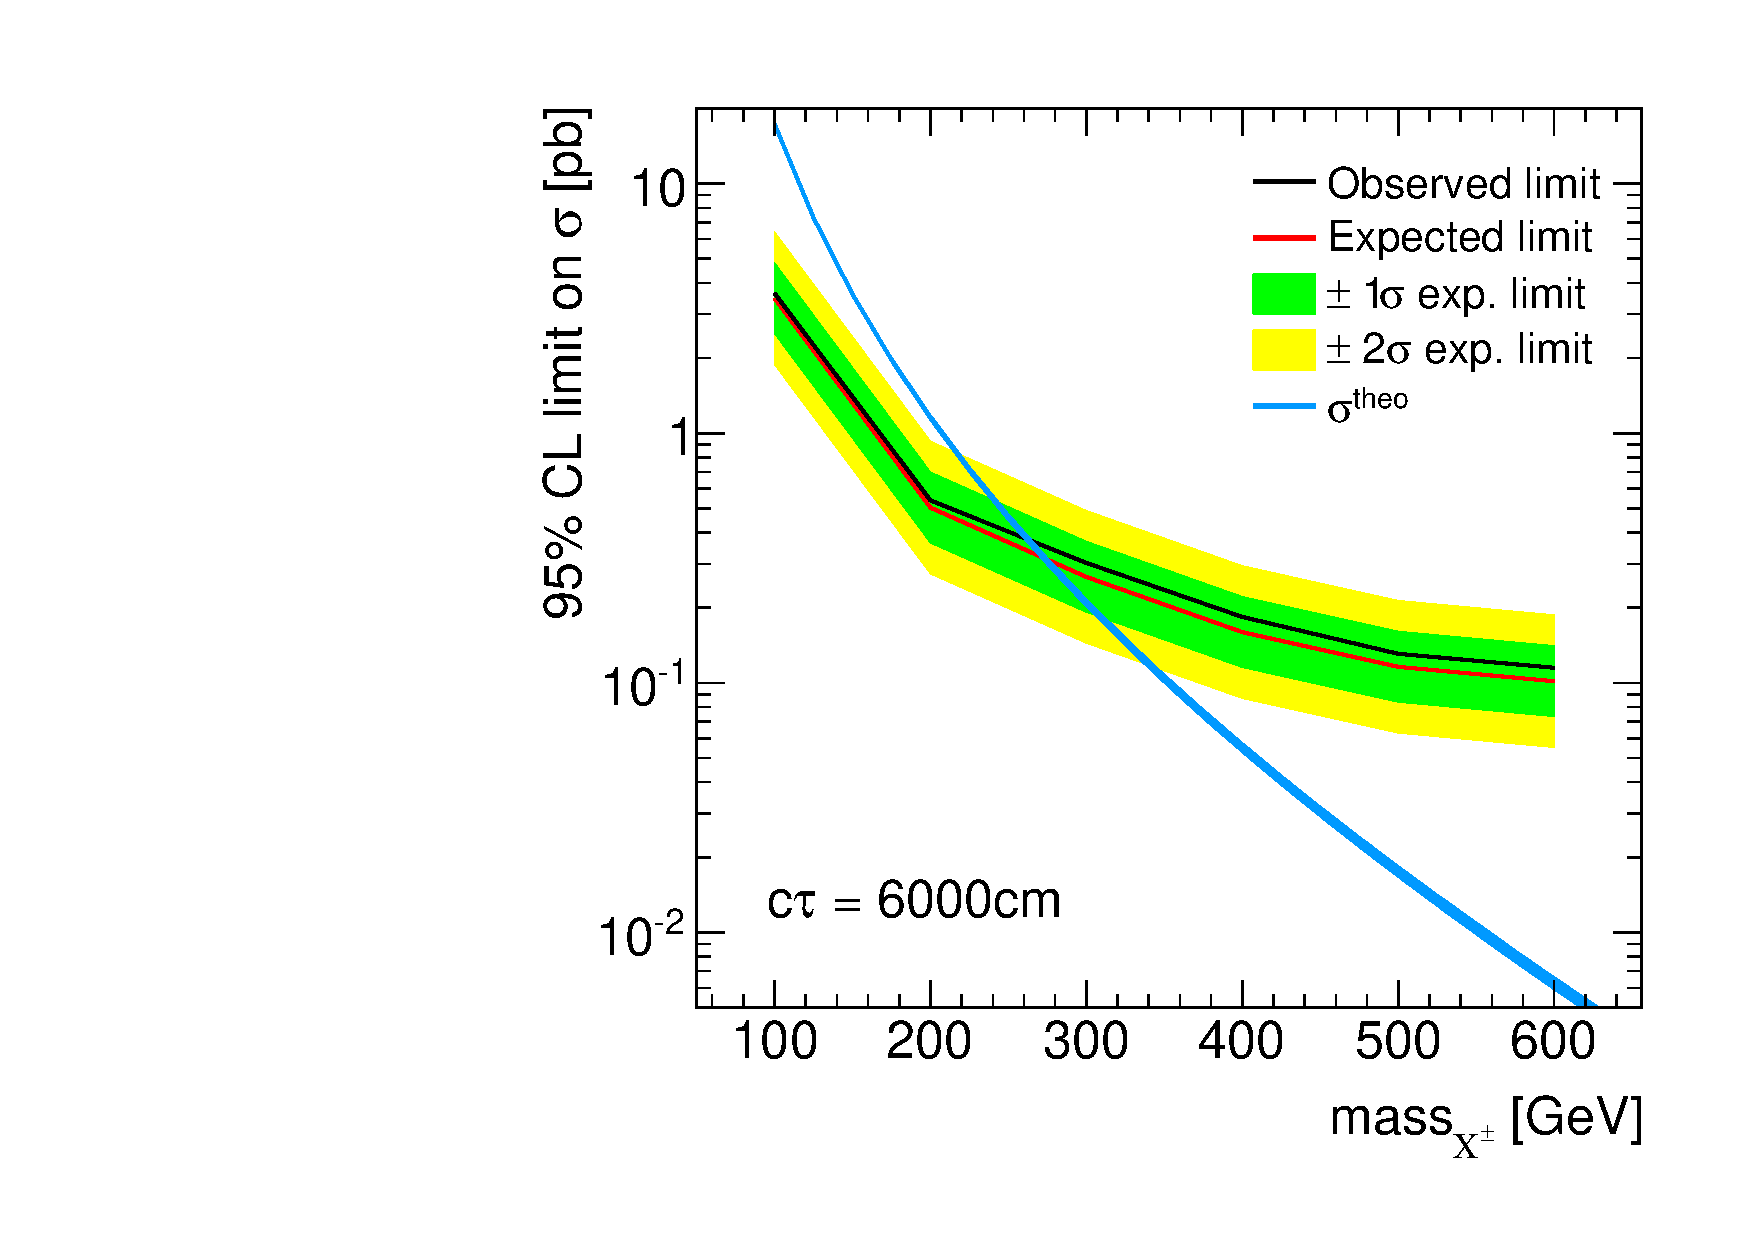
\includegraphics[width=0.29\textwidth]{figures/analysis/Interpretation/ExclusionLimits/LimitPlot_ctau6000cm.pdf} \\
    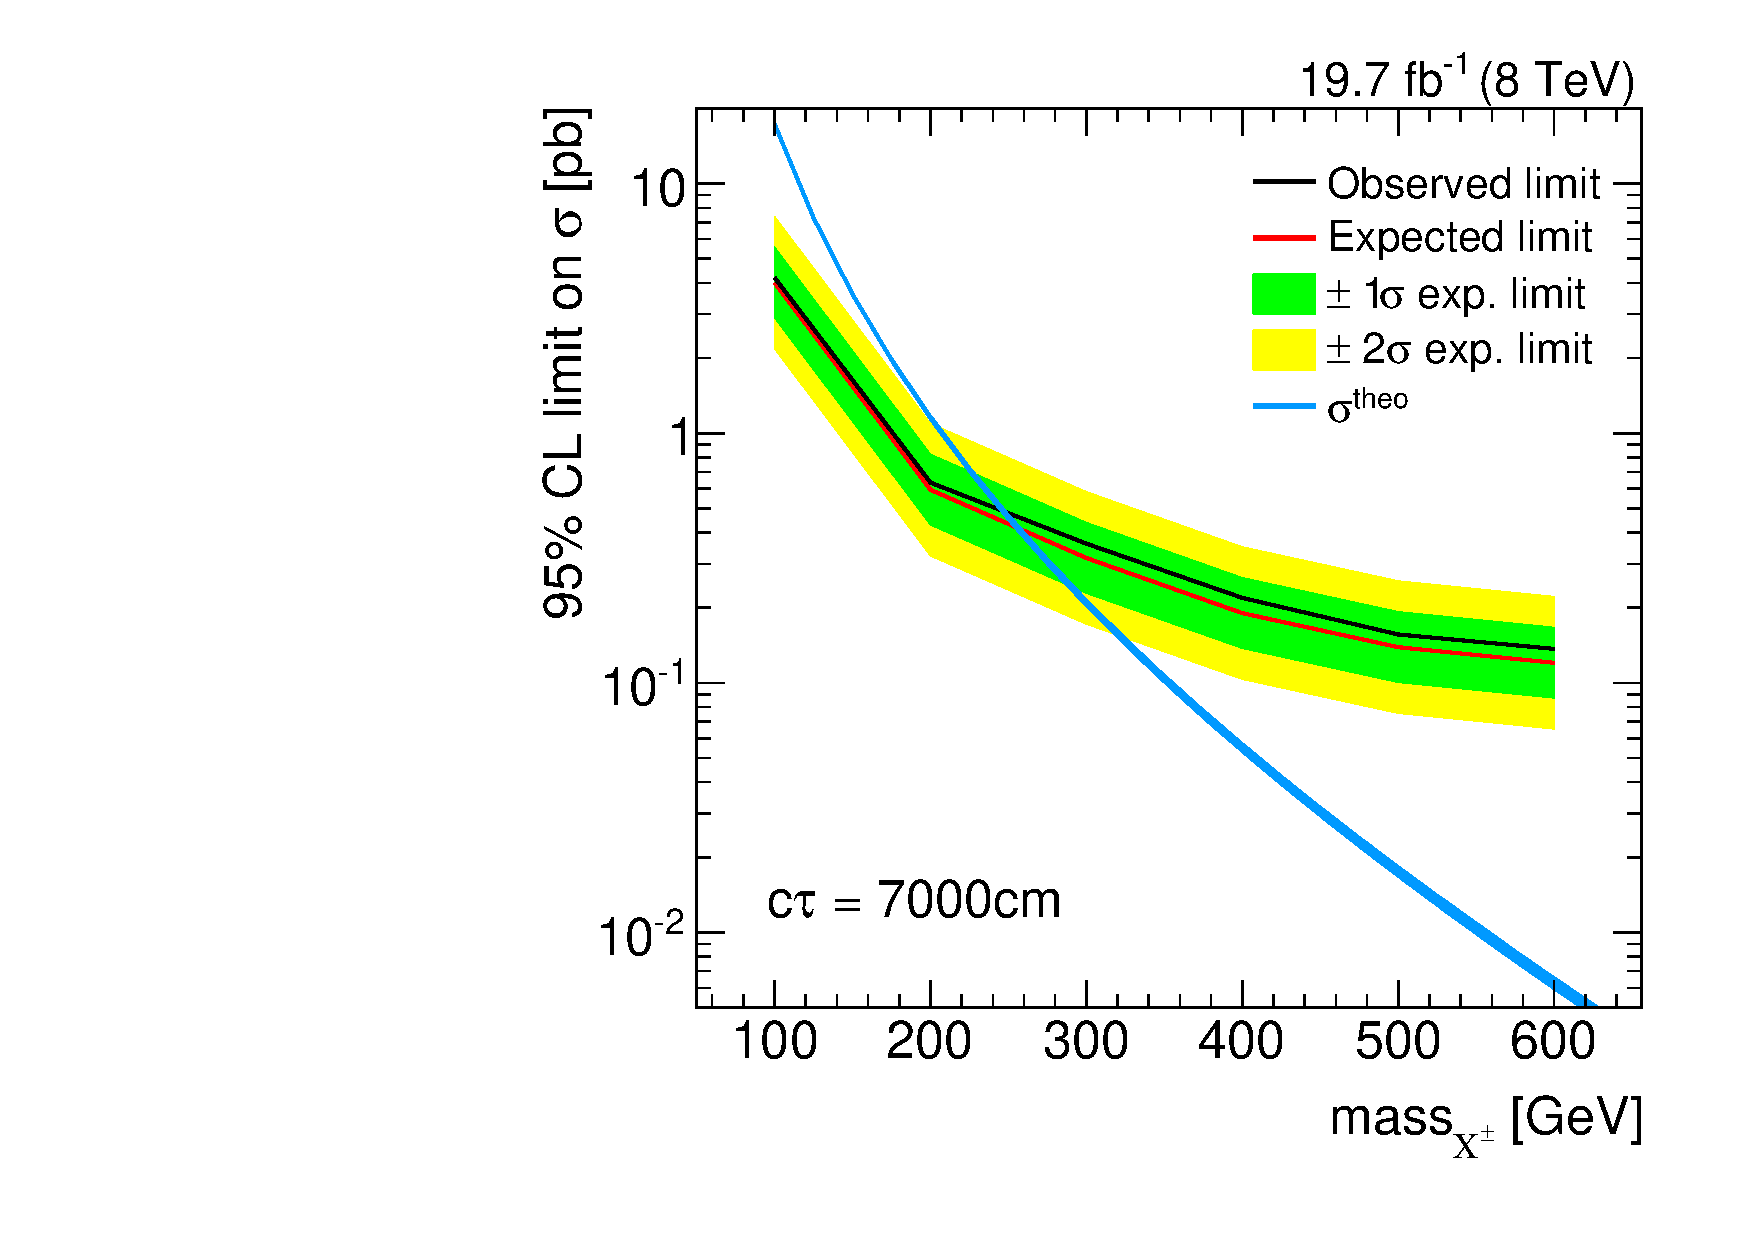
\includegraphics[width=0.29\textwidth]{figures/analysis/Interpretation/ExclusionLimits/LimitPlot_ctau7000cm.pdf} 
    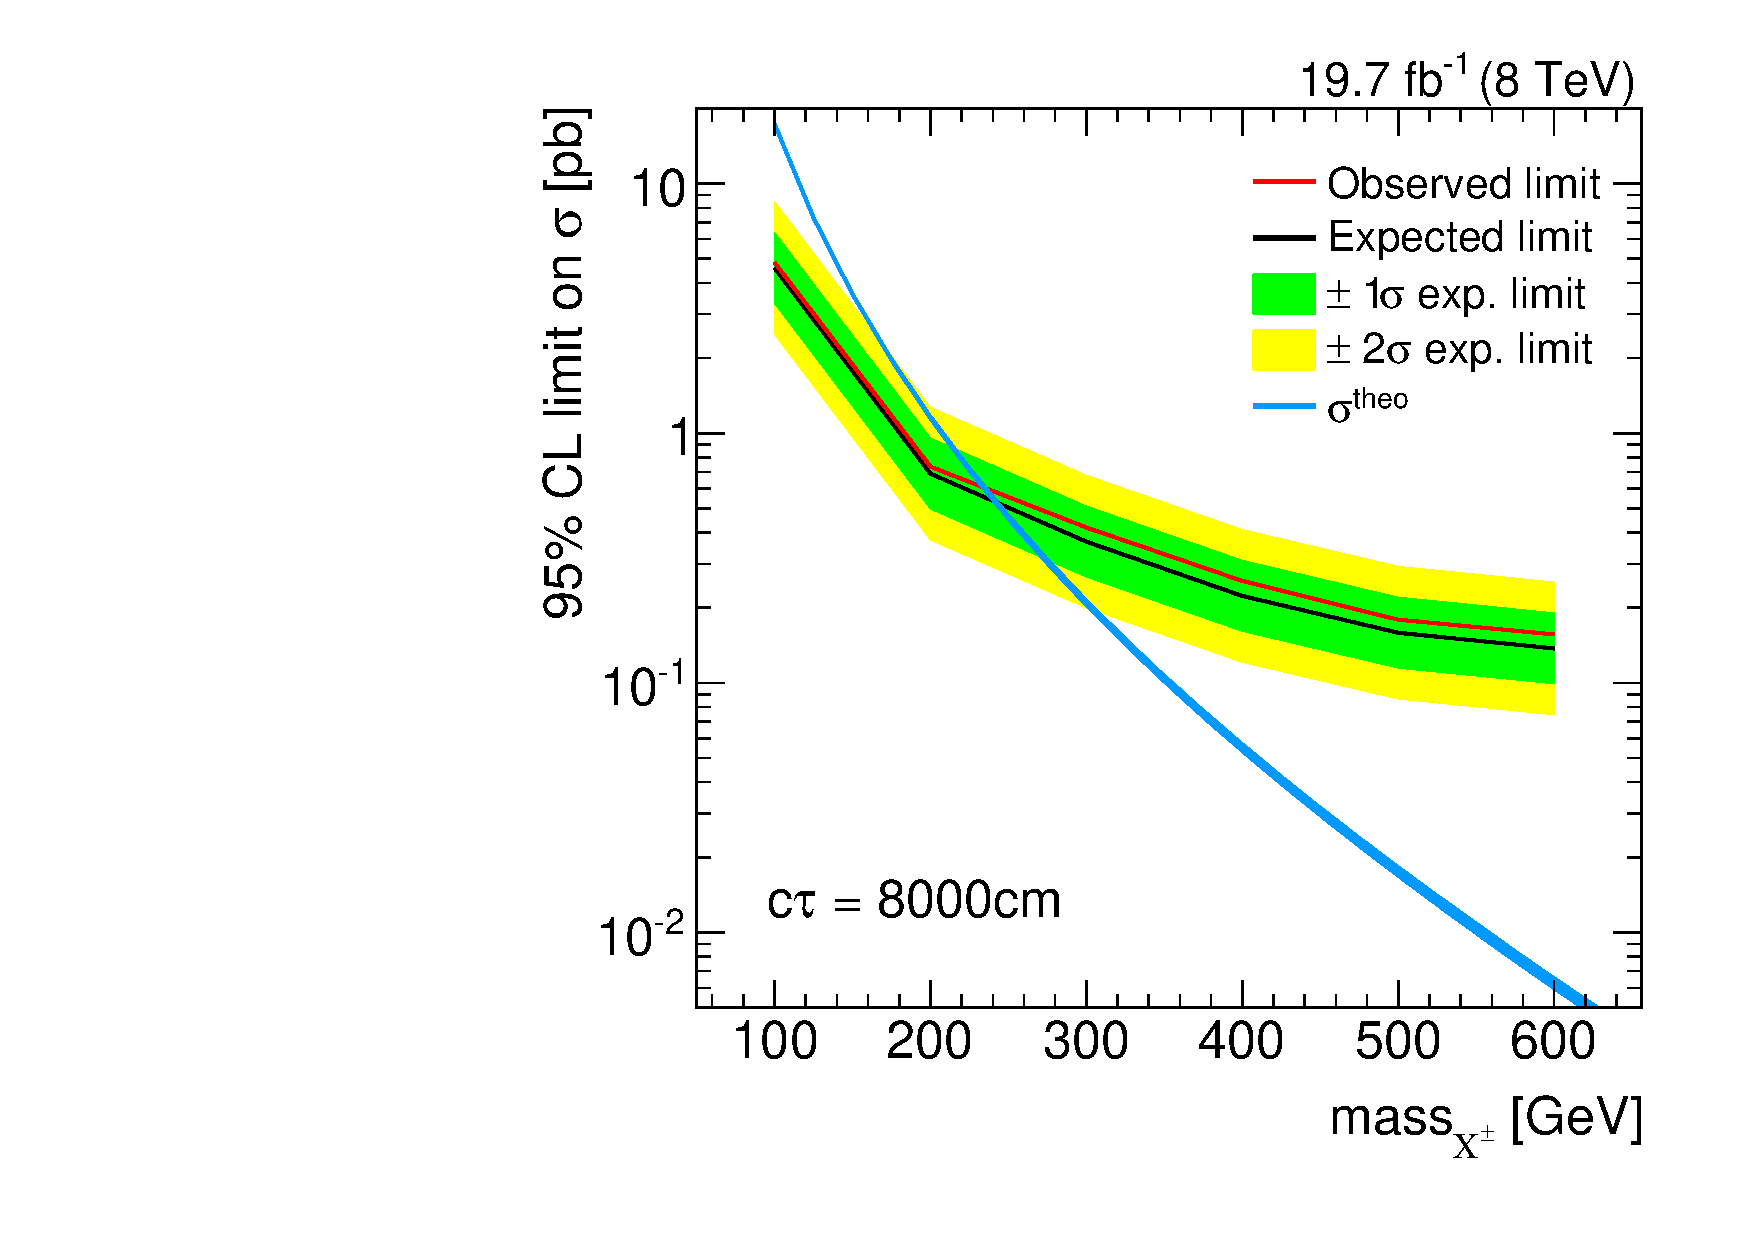
\includegraphics[width=0.29\textwidth]{figures/analysis/Interpretation/ExclusionLimits/LimitPlot_ctau8000cm.pdf} 
    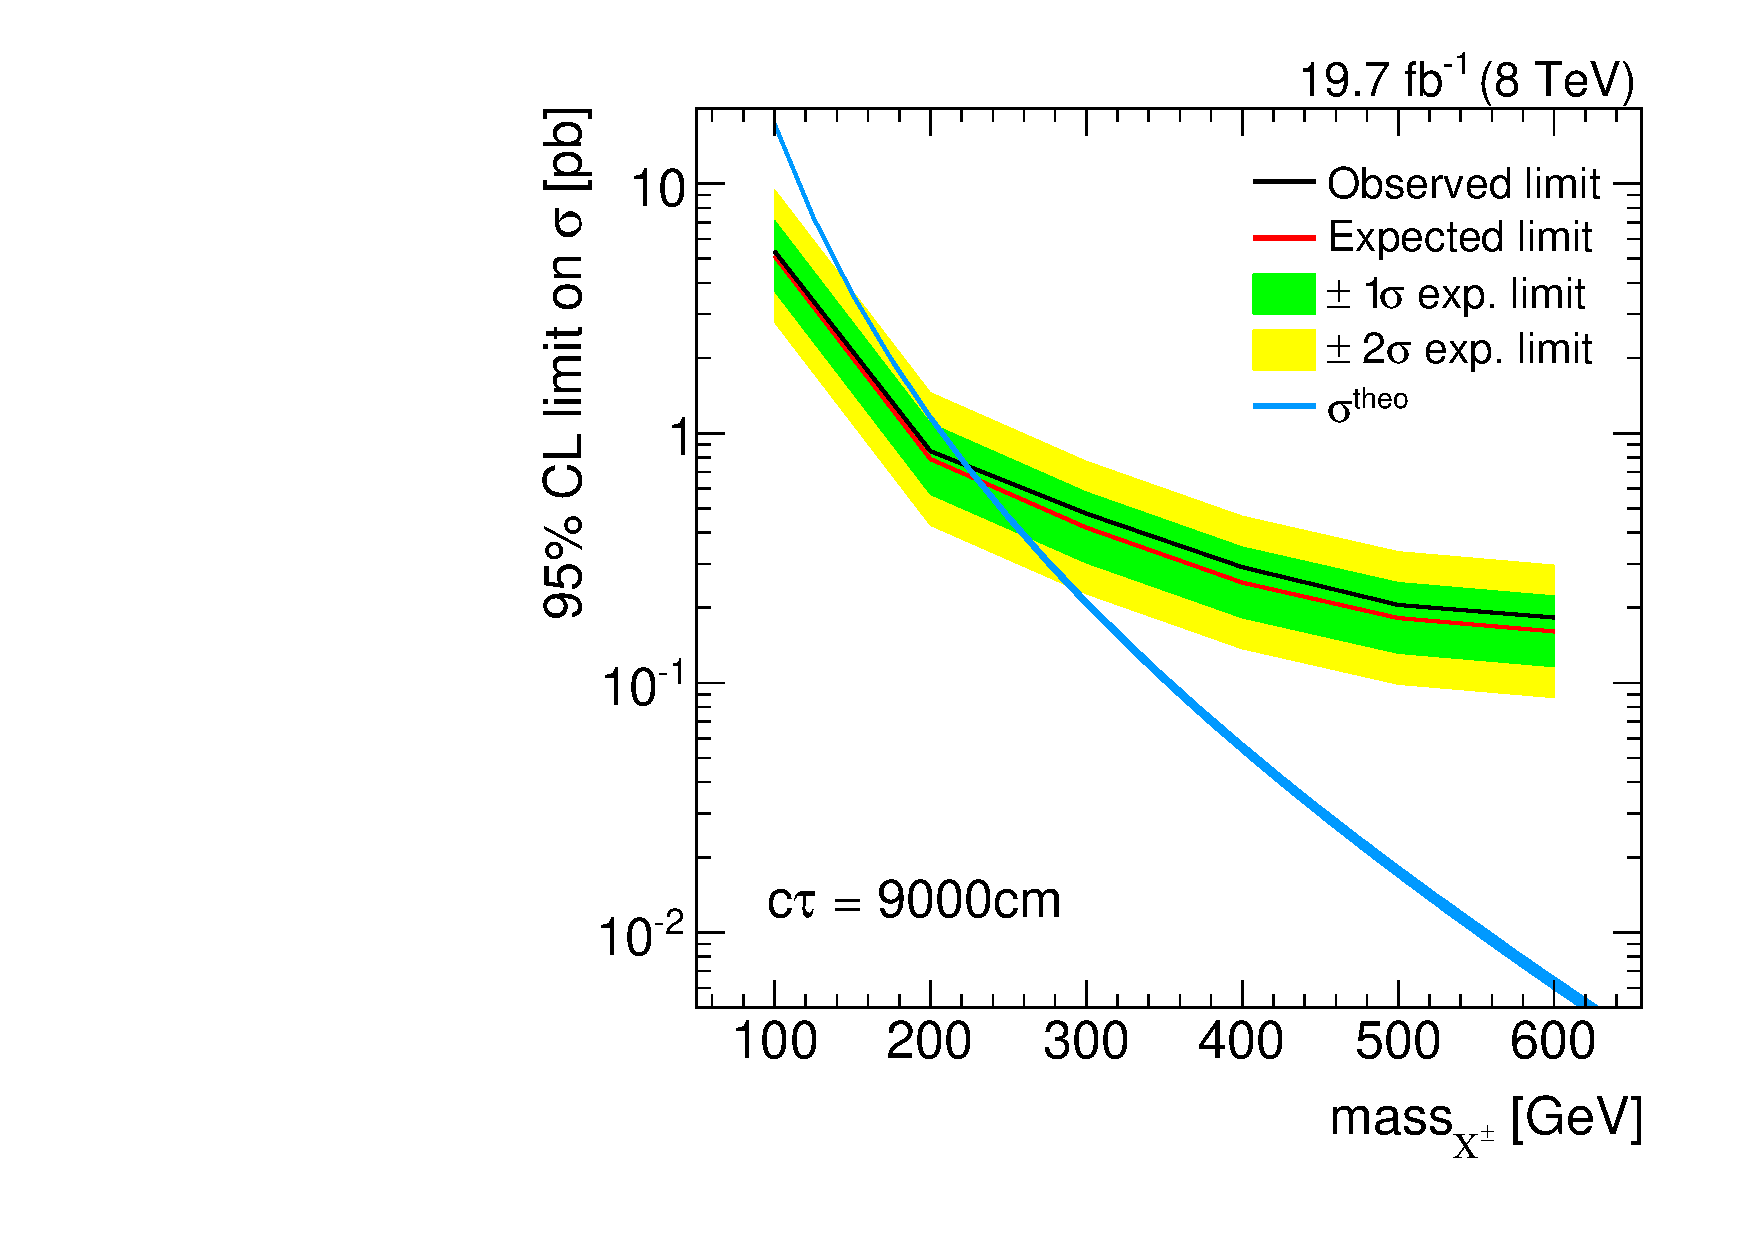
\includegraphics[width=0.29\textwidth]{figures/analysis/Interpretation/ExclusionLimits/LimitPlot_ctau9000cm.pdf} \\
  \end{tabular}
  \caption{95\% CL exclusion limits for signal models with $\ctau = 700-9000\cm$.}
  \label{fig:1dLimitsC}
\end{figure} 
